\newcommand{\Npe}{\ensuremath{N_\mrm{PE}}\xspace}

\chapter{Bonus: A Search for Milli-Charged Particles at the LHC}
{\small

\section{Motivation of a search for milli-charged particles}

One of the central mysteries of modern particle physics is the question of what
makes up dark matter. It must consist of massive particles that interact
at most very weakly with the SM, and no viable candidate exists among the
currently known particles. Moreover, a decade's worth of data from the LHC
has provided no evidence of any new particles that might provide an explanation.

We thus ask the question, what types of signatures might hypothetical dark matter
particles produce that would escape detection at present experiments?
One method of explaining dark matter is to add a new ``dark sector'' of
particles beyond the SM that couples only weakly to the SM. As an example,
we can add a ``dark photon'' $A'_\mu$ and a ``dark fermion'' $\psi'$ charged
under the new gauge field with charge $e'$. Allowing for kinetic
mixing between $A'_\mu$ and the SM weak hypercharge field $B_\mu$, the Lagrangian
for this new dark sector can be written
\be\label{eq:mcp_lagr}
\begin{split}
\mathcal{L}_\text{dark-sector} = &-\frac{1}{4}A'_{\mu\nu}A'^{\mu\nu} \\
&+i\bar{\psi}'(\gamma^\mu\partial_\mu + ie'\gamma^\mu A'_\mu + iM_\text{mCP})\psi' \\
&-\frac{\kappa}{2}A'_{\mu\nu}B^{\mu\nu},
\end{split}
\ee
where the first line is the kinetic term for a massless dark photon,
the second line contains the kinetic terms for a dark fermion with
mass $M_\mrm{mCP}$ as well as the interaction term with $A'_\mu$, and
the third line contains the mixing term between $A'_\mu$ and $B_\mu$, with
mixing strength parameter $\kappa$.

The mixing term can be eliminated by redefining $A'_{\mu\nu}\to A'_{\mu\nu}+\kappa B_{\mu\nu}$,
resulting in an interaction term $\kappa e'\bar{\psi}'\gamma^\mu B_\mu\psi$ between $\psi'$
and $B_\mu$. Rewriting $B_\mu$ in terms of the physical photon and $Z$ boson fields
as $B_\mu=\cos\theta_w A_\mu - \sin\theta_w Z_\mu$, we find that the new dark fermion
couples to the SM photon with electric charge $\kappa e'\cos\theta_w$, and couples to the 
SM $Z$ with charge $\kappa e'\sin\theta_w$. The mixing strength $\kappa$ must be small
(otherwise the new dark sector would have been observed already), so we must have
$\varepsilon\equiv \kappa e'\cos\theta_w/e \ll 1$, and we call $\psi'$ a
``milli-charged particle'' (mCP; note that the name is a bit of a misnomer because $\varepsilon$
does not have to be exactly $\mathcal{O}(10^{-3}$))

\begin{figure}[t]
  \begin{center}
    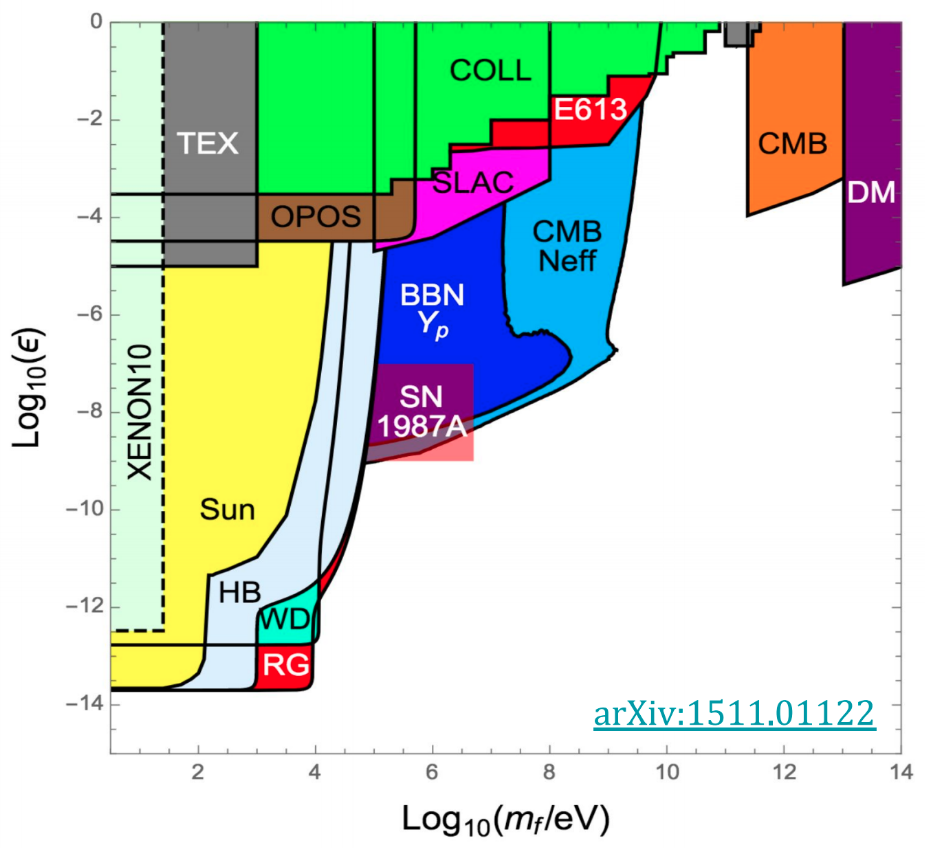
\includegraphics[width=0.50\textwidth]{figs/milliq/search_status.png}
    \caption{Existing exclusion limits for milli-charged particles, coming
      from searches via colliders, solar effects, astronomical observations,
      and cosmological bounds. milliQan targets the unexcluded phase space
      with $\varepsilon\geq10^{-3}$ and $10^{-1} < m_\text{mCP} < 10^2\GeV$.
      (Image from~\cite{Vinyoles:mcp})
            }
    \label{fig:mcp_search_status}
  \end{center}
\end{figure}

Such milli-charged particles have been searched for via a variety of methods,
either directly through collider experiments or indirectly through
solar effects, astronomical observations, or cosmological bounds.
A summary of the present exclusion space in the mCP mass--charge plane
is shown in Fig.~\ref{fig:mcp_search_status}, taken from~\cite{Vinyoles:mcp}.

There is a gap in the excluded phase space for $\varepsilon>10^{-3}$ at
the mass scales relevant at the LHC, roughly $10^{-1} < m_\text{mCP} < 10^2\GeV$.
mCPs at such masses and charges would be produced frequently at the LHC, but
present experiments would not be able to detect them; direct sensitivity is lost
for $\varepsilon$ below a few times $10^{-1}$, and a low cross section
precludes missing energy searches. Therefore, a dedicated experiment is necessary
to search for mCPs at the LHC.


\section{Overview of the milliQan detector}
The milliQan experiment, designed to search for mCPs using collisions at LHC P5, was proposed in 
2015~\cite{Haas:mcp,mq:loi}. It is located in a drainage gallery, elevated 45$^\circ$ above and 33
m from the CMS experiment, with 17 m of rock in between that naturally
suppresses beam-based backgrounds. The proposed design consists of four stacked ``layers'' of plastic 
scintillator arrays, with each scintillating bar coupled to a photomultiplier tube (PMT).
The arrays are pointed at the interaction point (IP), such that a particle originating
from a $pp$ collision would pass through all three layers in a straight line.
The bars are sensitive enough to detect individual photoelectrons produced by
throughgoing mCPs, and requiring a simultaneous hit in all three layers drastically
reduces background, which mostly consists of random overlap of pulses from
PMT dark rate, environmental radiation, cosmic rays, and afterpulsing.

The full milliQan design is anticipated to consist of four layers of $20\times20$ scintillator arrays,
each around 1 m$^2$ in total. In 2017--18, a smaller scale \textit{demonstrator} was installed
to study backgrounds and provide a proof-of-concept for the full-scale detector.
This demonstrator consists of three $2\times3$ scintillator bar arrays, roughly 1\%
of the planned full detector.

The 18 scintillator bars each measure 5 cm $\times$ 5 cm $\times$ 80 cm, and are
wrapped in layers of reflective and light-blocking materials to ensure optimal
efficiency. 3D-printed plastic casings couple the bars to individual PMTs
(two Hamamatsu R7725s, four Electron Tube 9814Bs, and 12 Hamamatsu R878s).

\begin{figure}[t]
  \begin{center}
    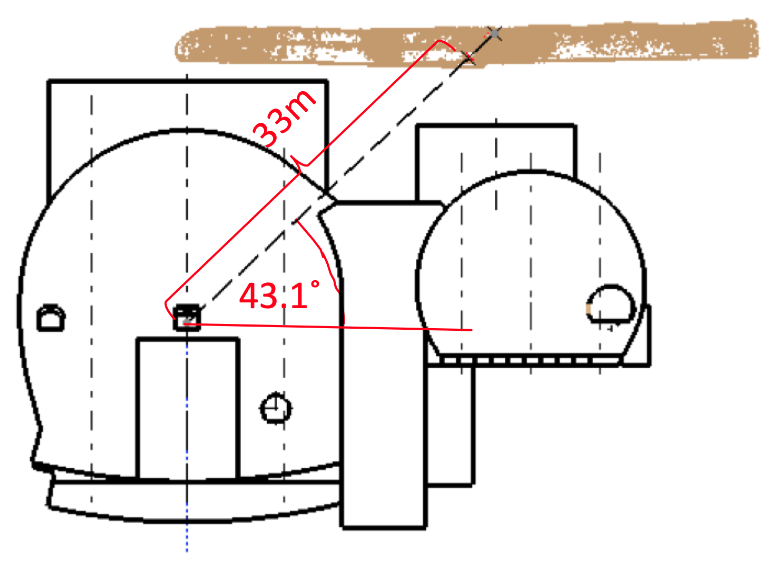
\includegraphics[width=0.440\textwidth]{figs/milliq/cavern_loc.png}
    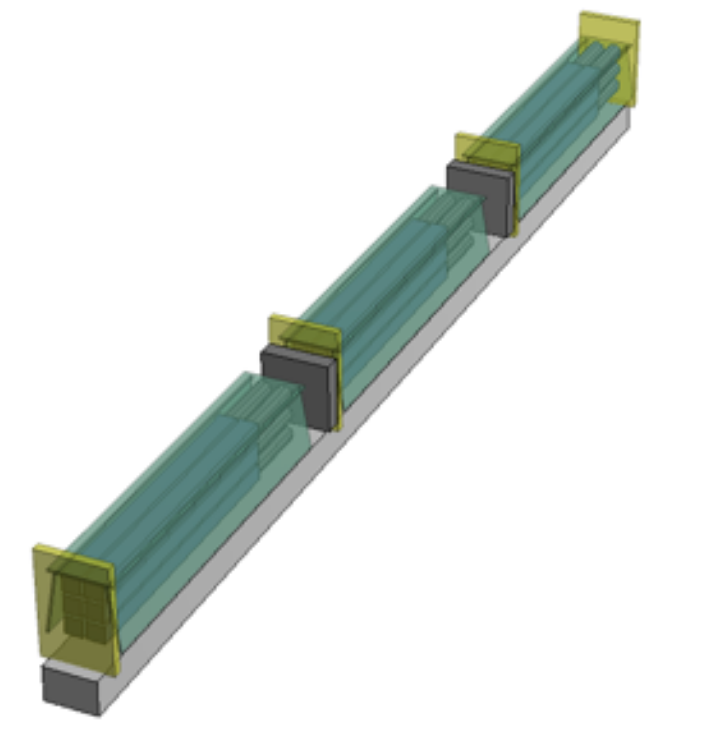
\includegraphics[width=0.352\textwidth]{figs/milliq/demonstrator_illustration.png}
    \caption{(left) Illustration of the location of the drainage gallery with 
      respect to the CMS cavern. CMS is located in the large dome on the left; 
      milliQan is elevated 43.1$^\circ$ above this, and 33 m away, with 17 m of
      rock in between. (right) 3D illustration of the demonstrator detector.
      The slabs are in yellow, the panels in translucent green, and the bars can be seen through
      the panels. The gray blocks in the layer gaps are lead bricks to block radiation.
            }
    \label{fig:demonstrator}
  \end{center}
\end{figure}

In addition to the scintillator bars, there are four 20 cm $\times$ 30 cm $\times$ 2.5 cm
scintillator ``slabs'' placed at the front and rear of the detector
as well as in between the layers, in order to tag/veto beam-based and cosmic
particles. Additionally, each layer has three 18 cm $\times$ 102 cm $\times$ 0.7 cm scintillator
``panels'' covering the top and sides, in order to tag/veto cosmic particles and environmental radiation.
Each of the slabs and panels is read out by a Hamamatsu R878 PMT.

There are 5 cm-thick lead bricks placed between each layer to reduce correlated pulses from radiation.
All of the scintillators and lead bricks are mounted on a custom-designed aluminum support structure
that can rotate the entire stack in multiple directions to facilitate alignment with the IP.
A CERN engineering team performed such an alignment, so that the detector points
to the IP to within a tolerance of just 1 cm over the 33 m distance. The location of the drainage gallery
and an illustration of the demonstrator are shown in Fig.~\ref{fig:demonstrator}.

The 31 scintillator channels are read out by a pair of CAEN V1743 digitizers, which sample at 1.6 GHz
and record a 640 ns waveform for each channel upon triggering. The trigger can be configured
to fire on single, double, or triple coincidence of peaks at an arbitrary threshold.
For nominal data taking, the trigger is set to fire on a triple coincidence of pulses.

\section{Bench tests for PMT calibration}
\label{sec:pmt_bench_tests}

The demonstrator detector makes use of three different ``species'' of PMTs, each of which
has very different characteristics. Even PMTs within the same species differ somewhat
in their behavior. It is therefore necessary to calibrate each PMT individually, so
that data can be interpreted correctly and simulation can be adjusted to accurately
model the behavior of the real detector.

Two separate calibrations are necessary. The first is the efficiency of the PMT
to convert an optical photon into a photoelectron (PE). Once installed in the detector, 
this is intertwined with the efficiency of the scintillators themselves to generate
and propagate the photons, so it is measured ``in-situ'', and described in the following
section. The other calibration involves the response of the PMT to a single photoelectron (SPE),
which includes the pulse shape and pulse area distribution. The mean pulse area
is also measured in-situ, as it can be affected by small magnetic fields and other effects,
but we perform measurements of the pulse shapes and full area distributions in the lab
using flashing LEDs, in order to (1) cross-check the in-situ measurements
and (2) generate the necessary inputs for the pulse-injection step of the simulation,
described in Sec.~\ref{sec:mq_mcgen}.

For the LED bench tests, we largely follow the method outlined in~\cite{Saldanha:pmt},
which allows for the measurement of the non-Gaussian low-area
tails of the SPE area distributions, arising from non-optimal trajectories
within the PMT (e.g. the photon skipping the cathode and directly hitting
the first dynode, or a photoelectron skipping a dynode stage).
The laboratory setup is sketched in Fig.~\ref{fig:pmt_setup}.
A blue LED and a PMT are placed in a light-tight enclosure,
and the LED is flashed in short $\sim$10 ns bursts so that the PMT
generates $\mathcal{O}(1)$ PE on average. The PMT is read out with
a DRS board~\cite{drs}, which is triggered on the LED pulse
so that even 0 PE events are recorded. An optional cardboard light-blocker
can be inserted between the LED and PMT, to collect a pure sample of 0 PE events.

\begin{figure}[t]
  \begin{center}
    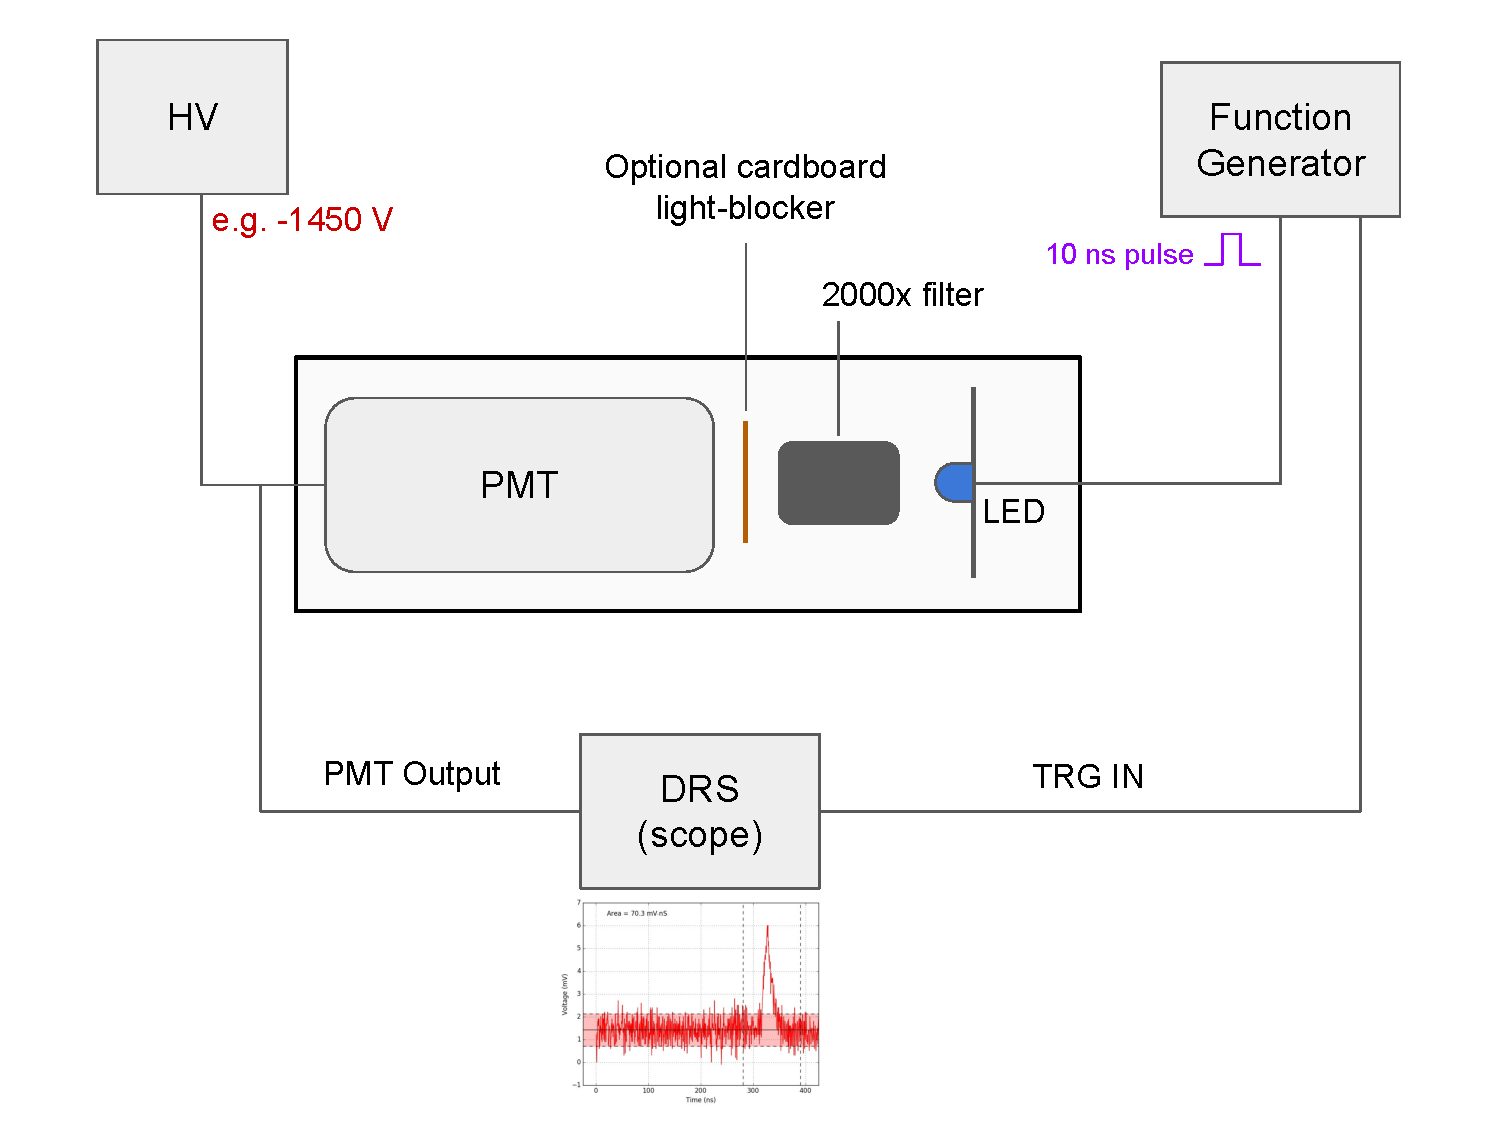
\includegraphics[width=0.650\textwidth]{figs/milliq/pmt_setup.pdf}
    \caption{Diagram of the laboratory setup for LED bench tests of the PMTs.
      An LED and the PMT are mounted in a light-tight 3D-printed casing,
      with a 2000x optical filter in between. The LED is flashed in
      short $\sim$10 ns pulses, and the PMT signal is read out by
      a DRS evaluation board~\cite{drs}. The board is triggered not by the 
      PMT but by the LED pulse generator, so that even ``blank'' (0 PE) events
      are recorded. An optional cardboard light-blocker can be inserted between
      the LED and PMT, in order to collect a pure sample of 0 PE events.
            }
    \label{fig:pmt_setup}
  \end{center}
\end{figure}

Upon each LED pulse, the PMT waveform is recorded. The pulse (when there is $\geq1$ PE)
occurs at the same time in each event, so there is no peak-finding necessary and the 
area can be computed by integrating over a fixed time window. The offset voltage level
and noise levels are estimated from the sideband before the pulse time window; this offset
is subtracted off before integrating to get the area. Doing this for many
events, one can build up a histogram of pulse areas, and if the LED intensity is
set correctly one can observed distinct peaks in the distribution corresponding
to 0, 1, 2,$\dots$ PE events. Fig.~\ref{fig:led_events} shows an example
R878 waveform and the pulse area distributions for a few different 
high-voltages (HVs).

\begin{figure}[t]
  \begin{center}
    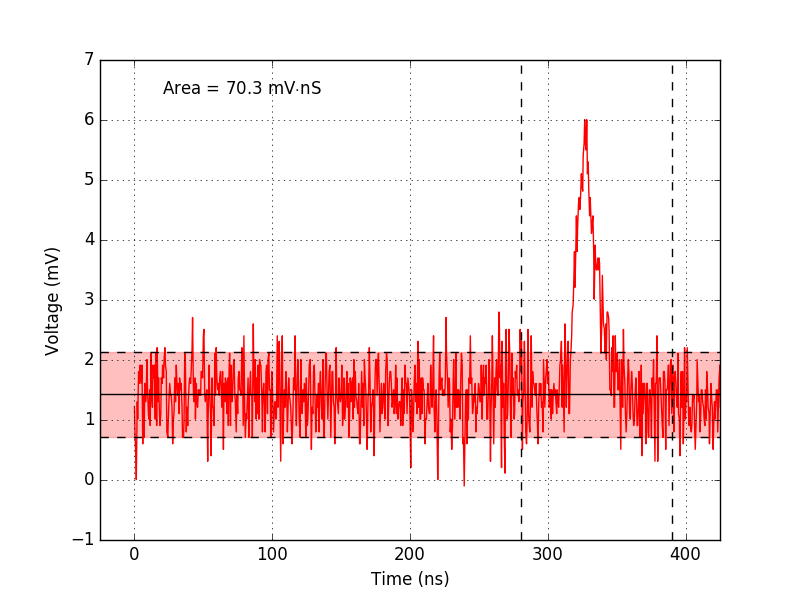
\includegraphics[width=0.450\textwidth]{figs/milliq/example_led_event_878.png}
    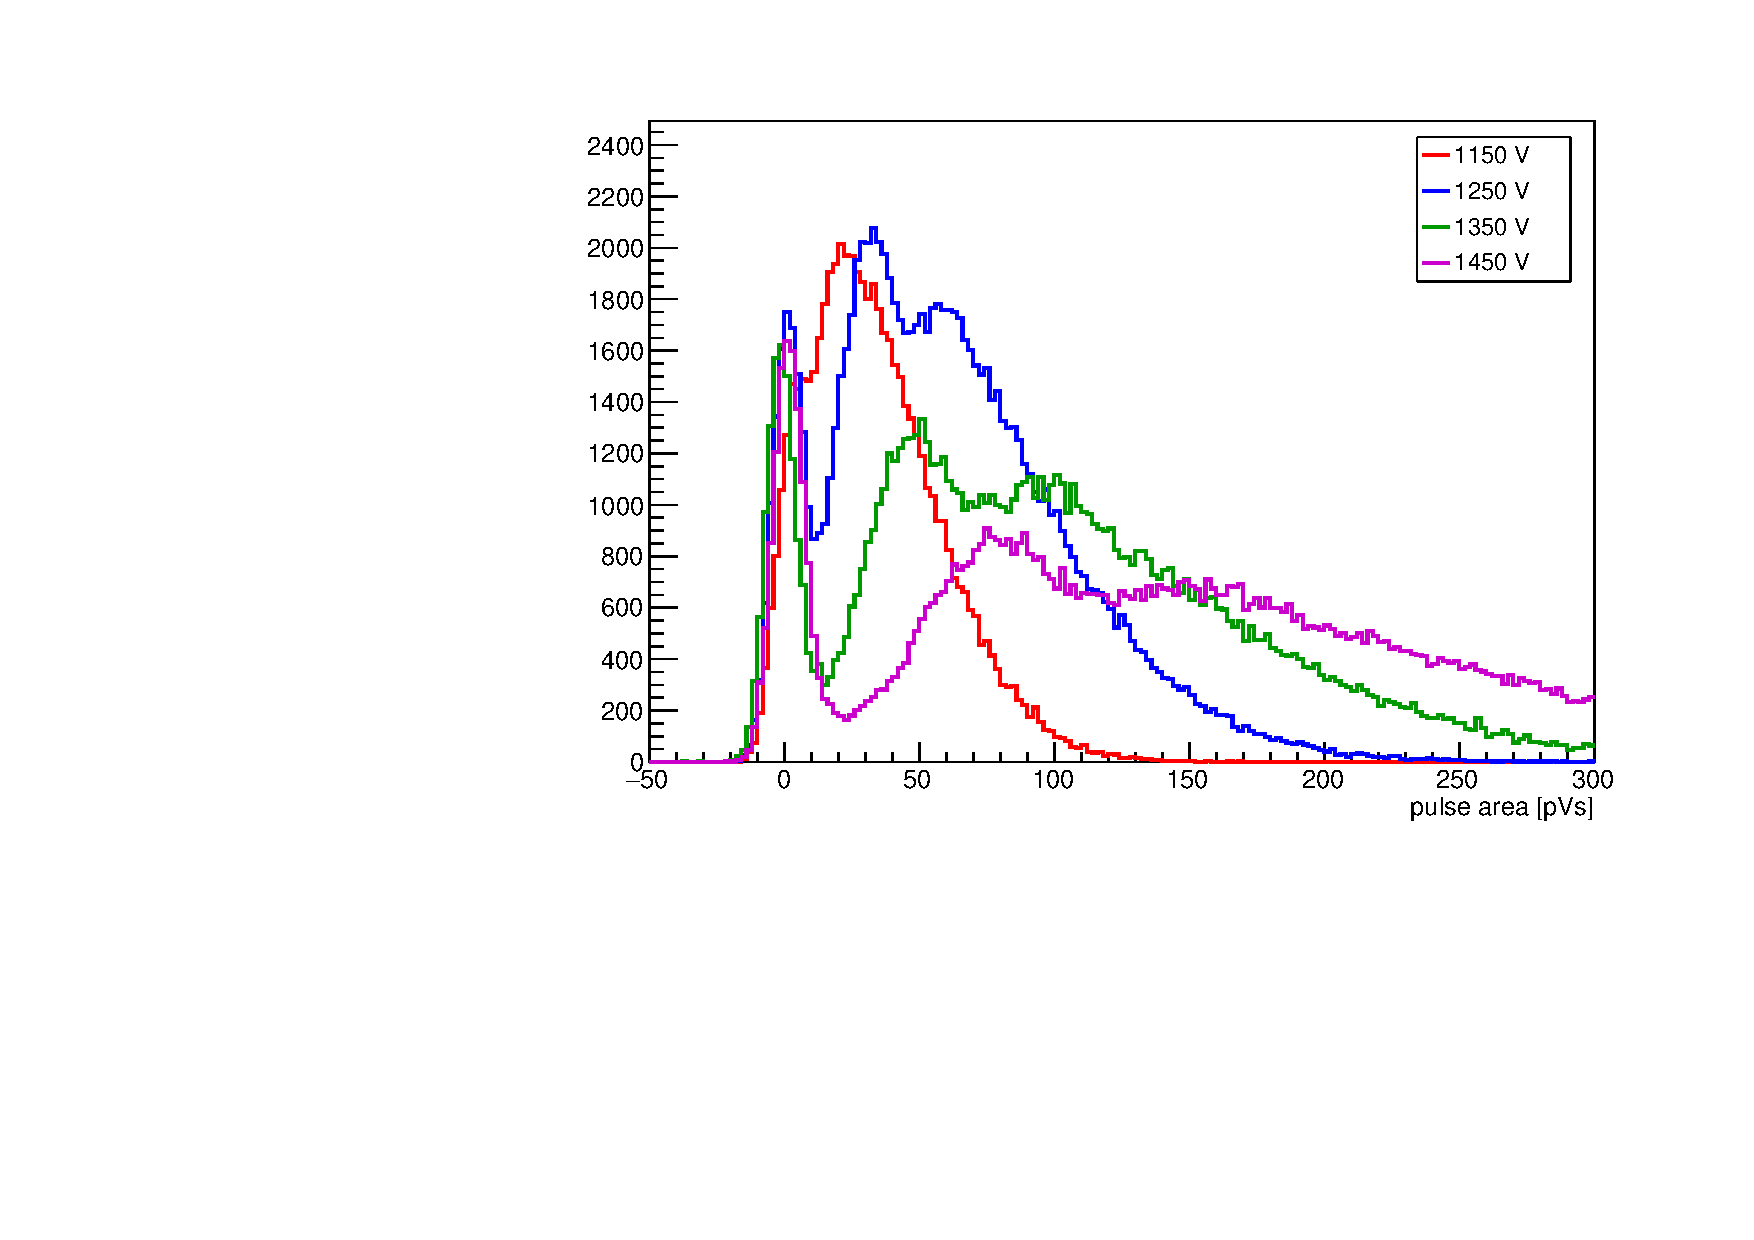
\includegraphics[width=0.500\textwidth]{figs/milliq/pmt_areas_hv_scan.pdf}
    \caption{(left) An example SPE waveform from and R878 PMT. The light red
      band shows the measured offset ($\sim$1.4 mV) and noise level ($\pm$0.6 mV).
      The vertical dashed lines indicate the fixed time window in which the 
      waveform is integrated to compute the pulse area.
      and (right) the pulse area distributions
      for a variety of HVs, for an R878 PMT. The LED intensity is set so that
      the average number of PE is near 1, so one can resolve distinct peaks for
      0, 1, and 2 PE events in the area distributions. As the HV is increased, the peaks
      move to the right.
            }
    \label{fig:led_events}
  \end{center}
\end{figure}

The actual calibration method makes use of the fact that the number of observed photoelectrons
after the LED light is heavily filtered is a Poisson process. Two datasets are recorded:
one with no cardboard light-blocker, and the LED intensity set so that there
is $\mathcal{O}(1)$ PE on average per event, and one with the light-blocker inserted
(but with the LED running at the same intensity, so that any electronic effects
are still captured).

The LED-blocked dataset is a pure sample of 0 PE events, and the resulting pulse area distribution
(which is just a Gaussian near 0) can be scaled to fit the left edge of the area distribution
of the non-blocked dataset. It is important to fit only the left edge, and not the full 0-PE peak,
as the right side can have contributions from sub-optimal 1 PE events. By taking the ratio
of the areas of the scaled LED-blocked histogram and the non-blocked histogram, one can get
the fraction $f_0$ of 0 PE events. Since \Npe is Poisson, we can then compute the
mean and variance as
\be
\text{Var}(\Npe) = \langle \Npe\rangle = -\log(f_0).
\ee

Once we have this, it is straightforward to compute the mean and variance
of the area distribution of an SPE pulse. Denoting $A_\mrm{SPE}$ as the area distribution of an SPE
pulse, $A_\mrm{nb}$ as the area distribution of the non-blocked dataset, and $A_\mrm{b}$ as
the area distribution of the LED-blocked dataset, the mean and variance are given by
\be\label{eq:mean_spe}
\langle A_\mrm{SPE}\rangle = \frac{\langle A_\mrm{nb}\rangle - \langle A_\mrm{b}\rangle}{\langle \Npe \rangle}
\ee
\vspace{-4mm}
\be\label{eq:var_spe}
\mrm{Var}(A_\mrm{SPE}) = \frac{\mrm{Var}(A_\mrm{nb}) - \mrm{Var}(A_\mrm{b})}{\langle \Npe \rangle} - \langle A_\mrm{SPE}\rangle^2
\ee
(the variance equation is not trivial, see \cite{Saldanha:pmt} for details).

\begin{figure}[t]
  \begin{center}
    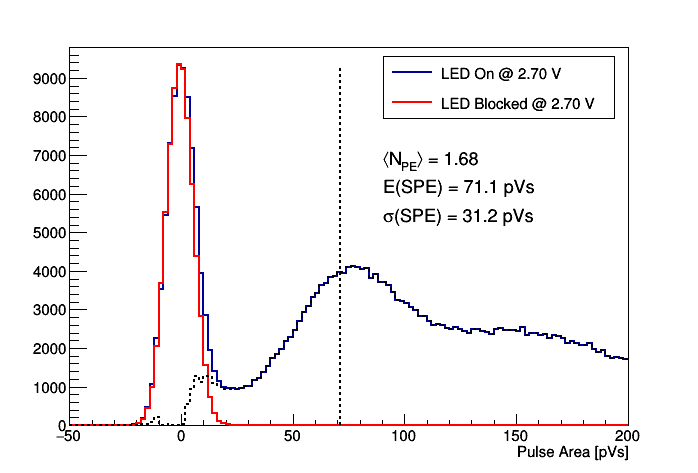
\includegraphics[width=0.480\textwidth]{figs/milliq/calib_example_878.png}
    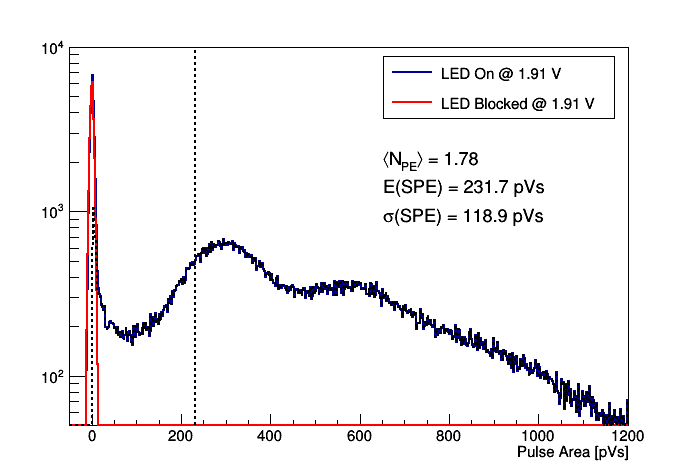
\includegraphics[width=0.480\textwidth]{figs/milliq/calib_example_7725.png}
    \caption{Example calibrations for an R878 (left) and R7725 (right). The dark
      blue histograms are pulse area distributions from the nominal LED setup,
      and the red histograms are area distributions with the LED blocked by cardboard.
      This red histogram is scaled to fit the left edge of the navy histogram in order to estimate
      the 0 PE component. Since the distribution of \Npe is Poisson, the fraction
      of 0 PE events can be used to compute $\langle \Npe\rangle$, from which one
      can get the mean and standard deviation of the SPE area distribution. The vertical
      dotted line indicates the computed mean, notably lower than the 1-PE peak
      due to the large non-Gaussian low-area tails.
            }
    \label{fig:pmt_calib}
  \end{center}
\end{figure}

Fig.~\ref{fig:pmt_calib} shows an example of this process for an R878 and R7725. The dark
blue histograms are the non-blocked area distributions, and the red histograms are the
LED-blocked area distributions. The red histograms are scaled to fit the left edge of the
blue histograms, and then used to find $\langle \Npe\rangle$. The Eqs.~\ref{eq:mean_spe}
and \ref{eq:var_spe} are used to compute the mean and variance of the SPE area distribution.
Note in particular that the means are noticeably lower than the peaks from 1-PE events.
This is due to the large non-Gaussian low-area tails in the SPE response, visible
as the dotted histogram (just the subtraction of red from blue).

\begin{figure}[t]
  \begin{center}
    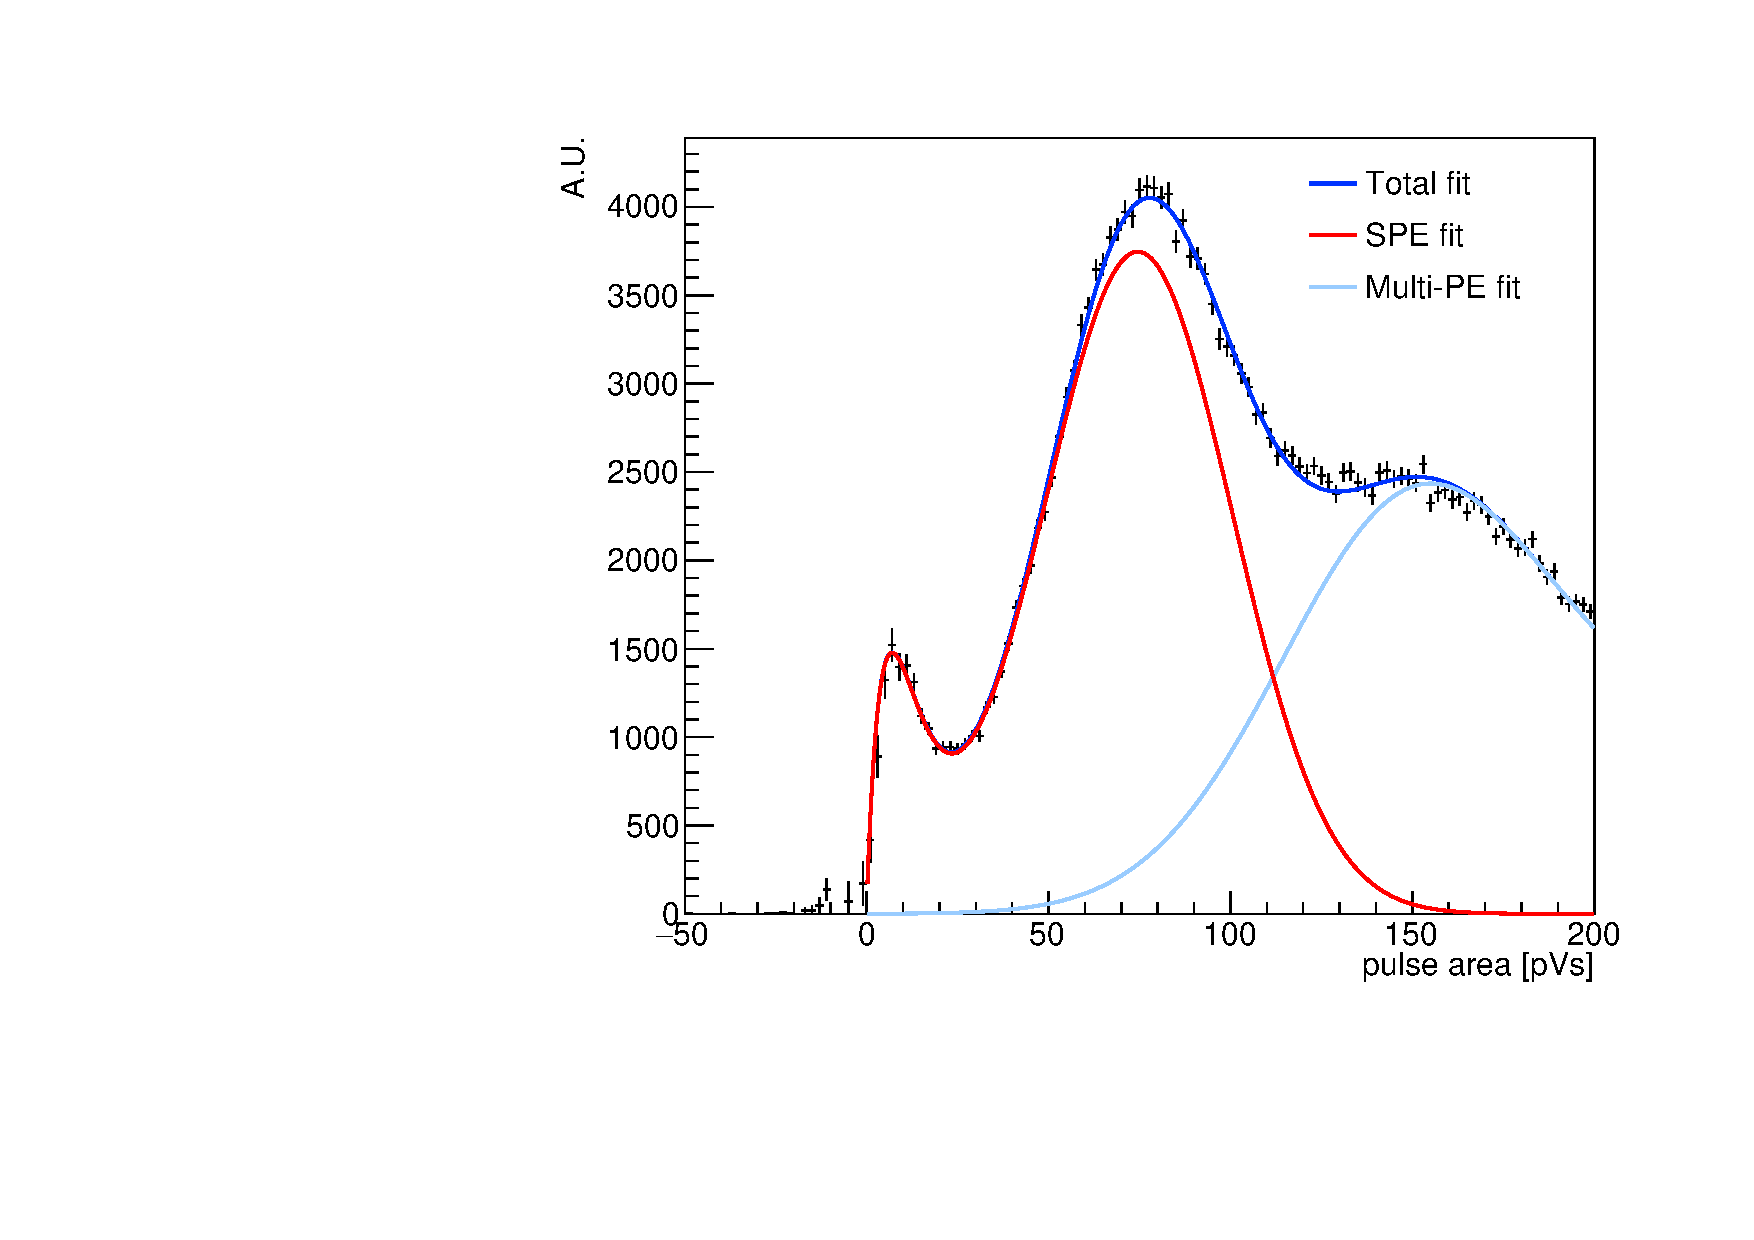
\includegraphics[width=0.325\textwidth]{figs/milliq/area_dist_878.pdf}
    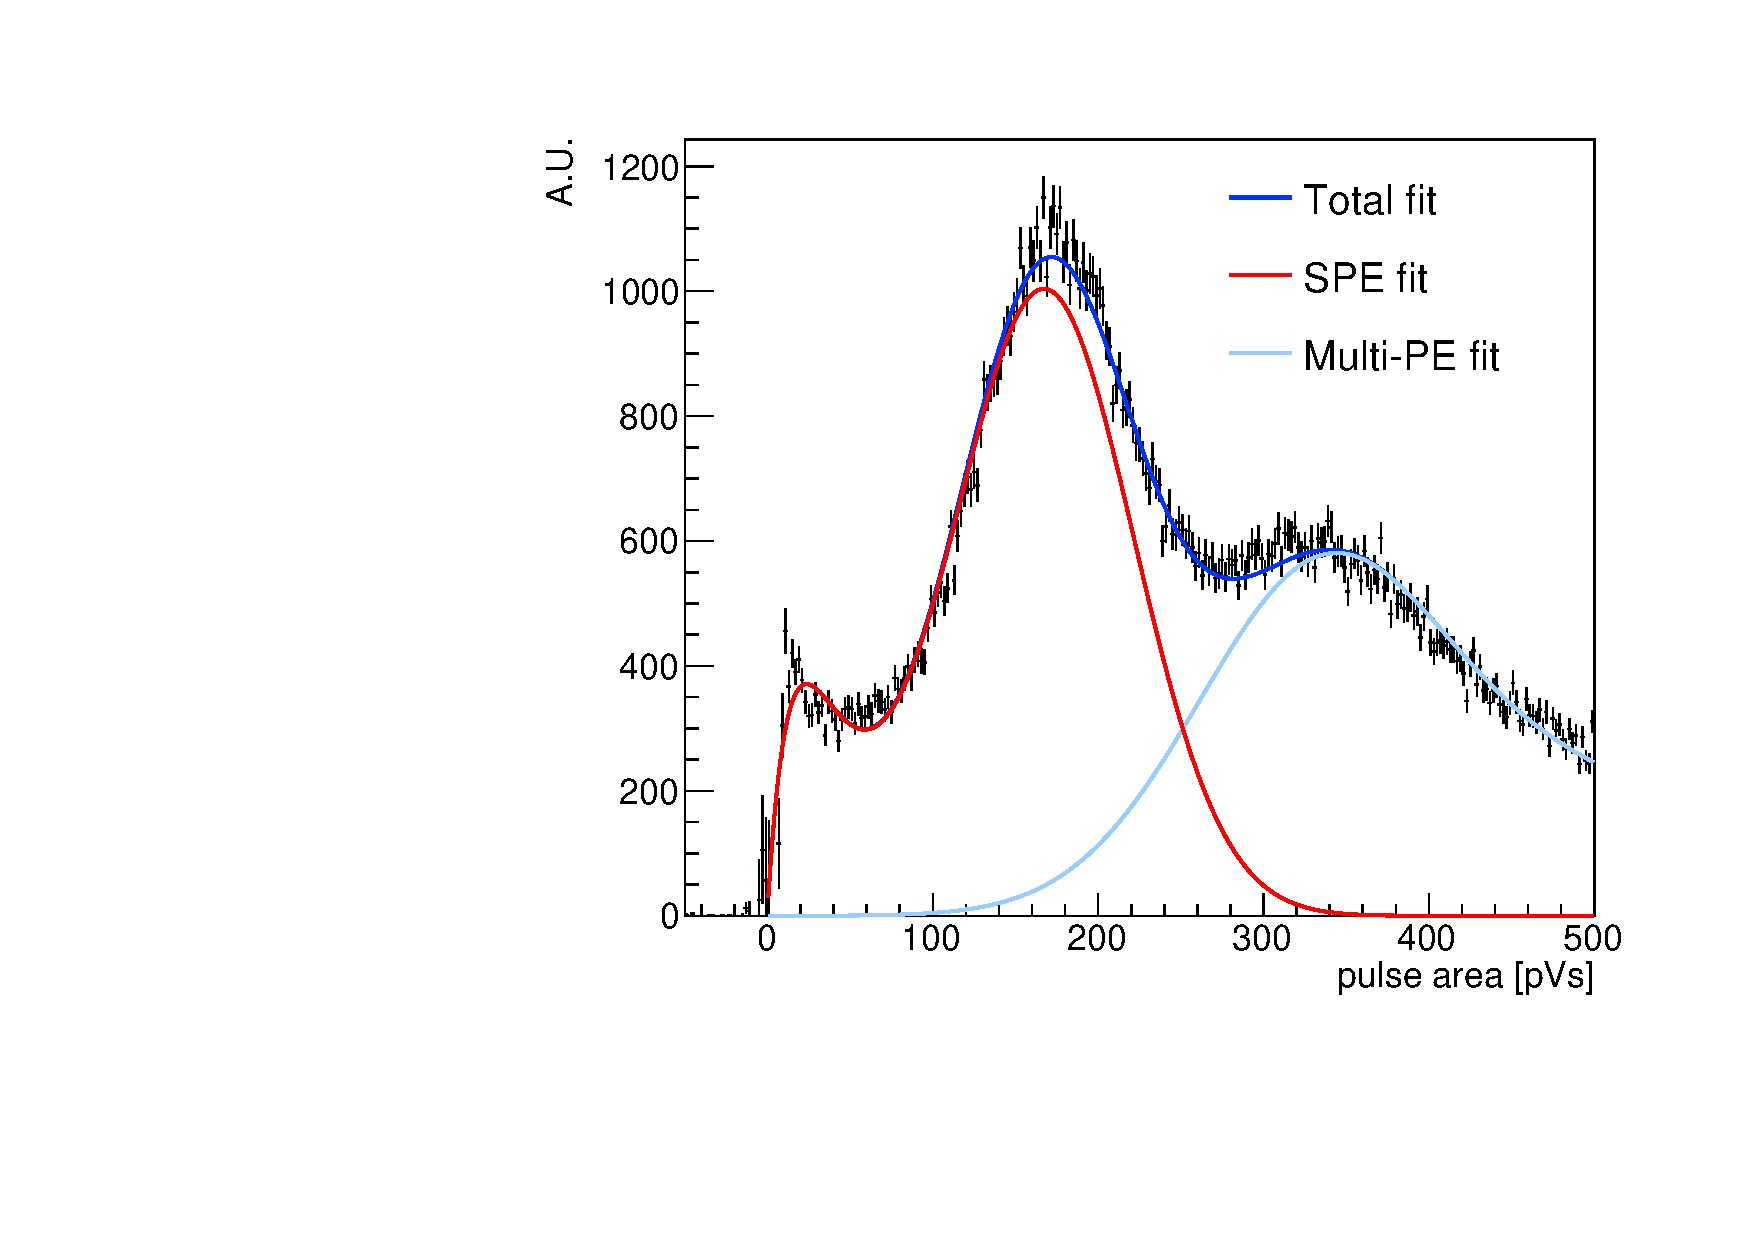
\includegraphics[width=0.325\textwidth]{figs/milliq/area_dist_7725.pdf}
    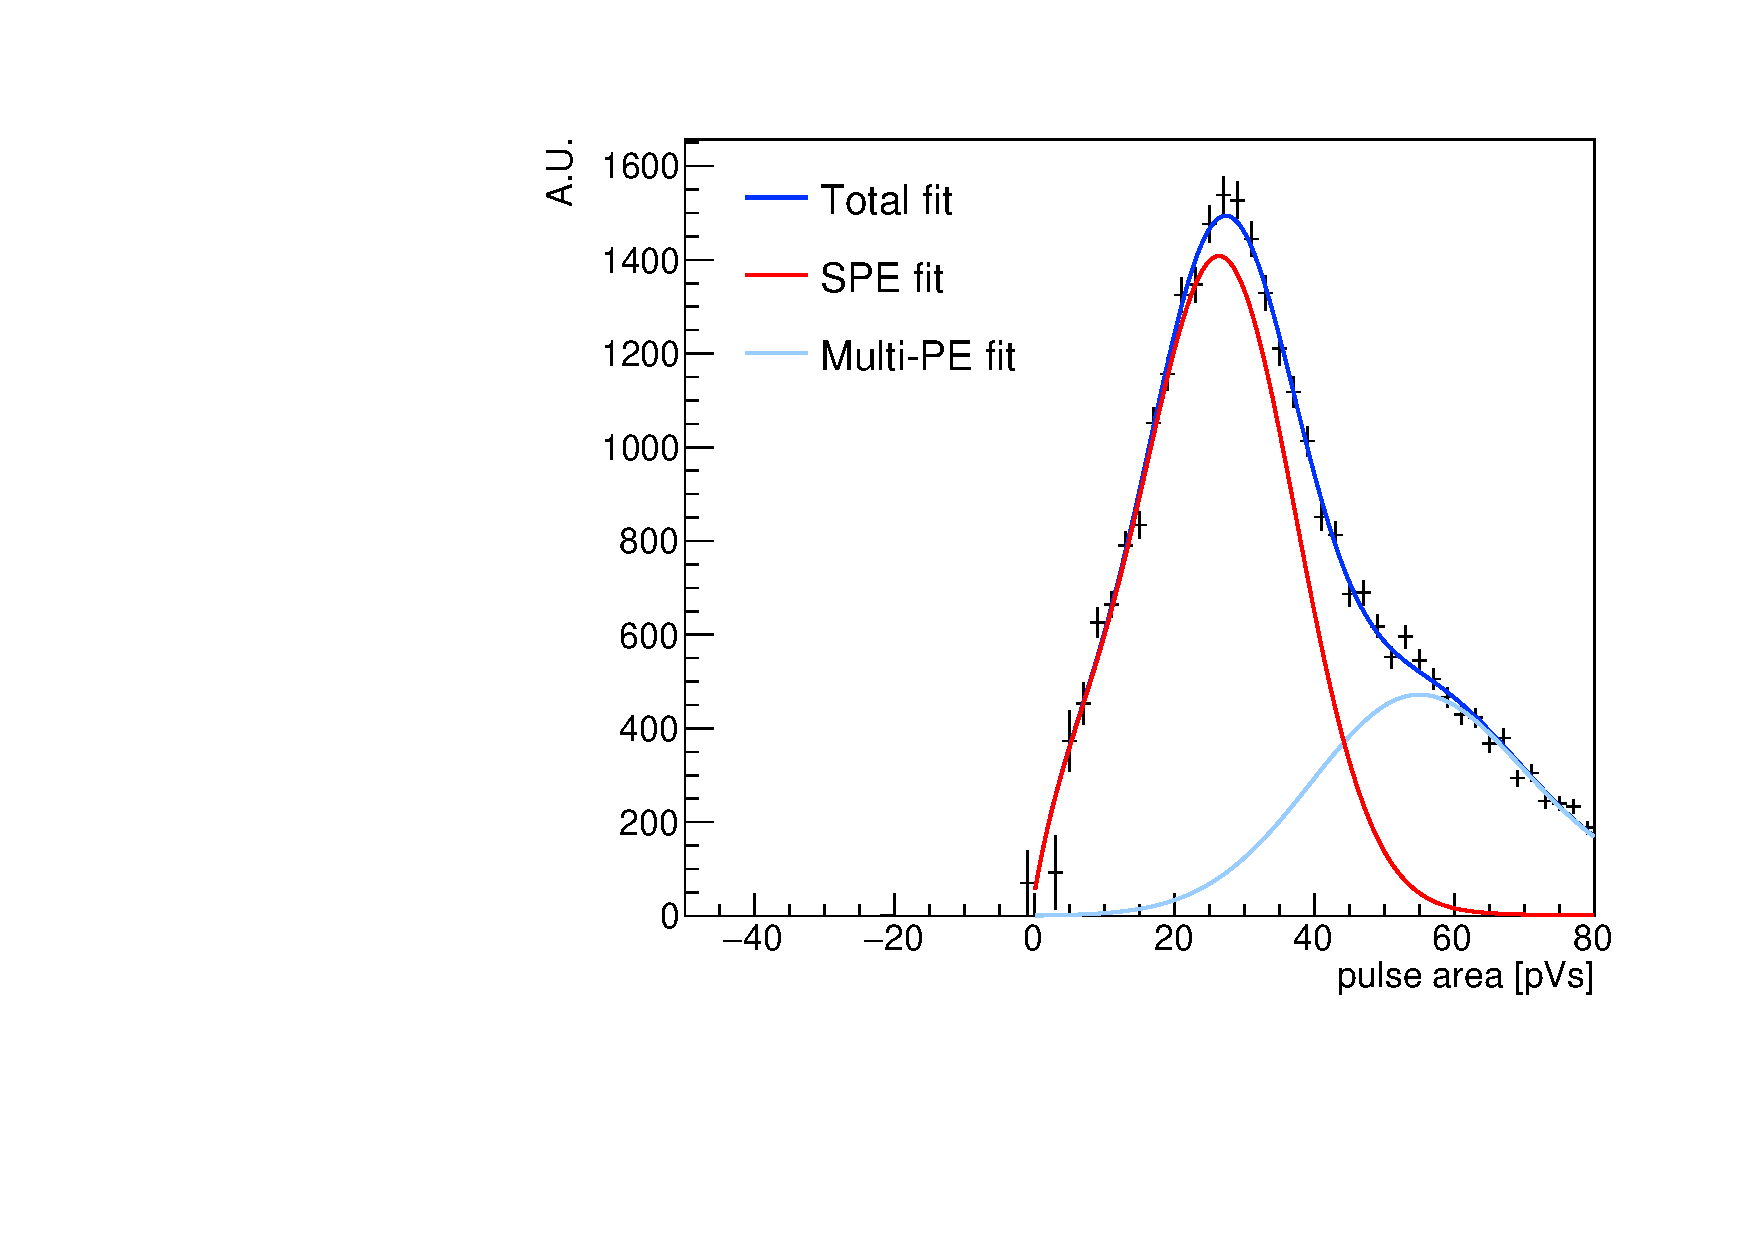
\includegraphics[width=0.325\textwidth]{figs/milliq/area_dist_ET.pdf}
    \caption{Measured area distributions for the R878, R7725, and ET
      (at 1450, 1400, and 1700 V),
      after subtracting off the 0-PE component.
      Black points are the raw 0 PE-subtracted area distributions.
      The red curve is the fitted SPE response (modeled as Guassian plus
      exponential left tail, given in Eq.~\ref{eq:spe_func}), and the light blue curve is the fitted
      multi-PE response (one Gaussian each for 2- and 3-PE components).
      The red curve is used to draw random areas during pulse injection,
      described in Sec.~\ref{sec:mq_mcgen}.
            }
    \label{fig:area_dists}
  \end{center}
\end{figure}

In addition to the mean SPE response that is used to calibrate each
individual PMT, we are also interested in the full \textit{distribution}
of areas for an SPE, in order to use them for pulse injection, described
in Sec.~\ref{sec:mq_mcgen}. To do this, we subtract the scaled LED-blocked
area distribution from the nominal non-blocked distribution,
to get the area distribution of events with $\geq$1 PE. We then simultaneously
fit the 1 PE and $>$1 PE distributions to this histogram. The SPE response
is modeled as a Gaussian plus exponential left tail, with PDF given by
\be\label{eq:spe_func}
\psi_\mrm{SPE}(x) = G(\mu,\sigma)(1-e^{-x/a})e^{-x/b},
\ee
where $G(\mu,\sigma)$ is a standard Gaussian, and $\mu$, $\sigma$, $a$, and $b$
are free parameters to be fit. The multi-PE response is modeled as a sum
of Gaussians, with means $n\mu$ and standard deviations $\sqrt{n}\,\sigma$,
where $n$ is the number of PE (we only consider up to $n=3$). We then fit
all four parameters simultaneously, and take $\psi_\mrm{SPE}$ as the pulse
area distribution for SPEs to be used for pulse injection. 
The fitted functions for all three types of PMTs are shown in Fig.~\ref{fig:area_dists}.

One final piece of information that we need to extract from the LED tests are SPE pulse shape
templates for all PMT types. Like the above, these are used during pulse injection, described
in Sec.~\ref{sec:mq_mcgen}. The procedure is as follows:

\begin{figure}[t!]
  \begin{center}
    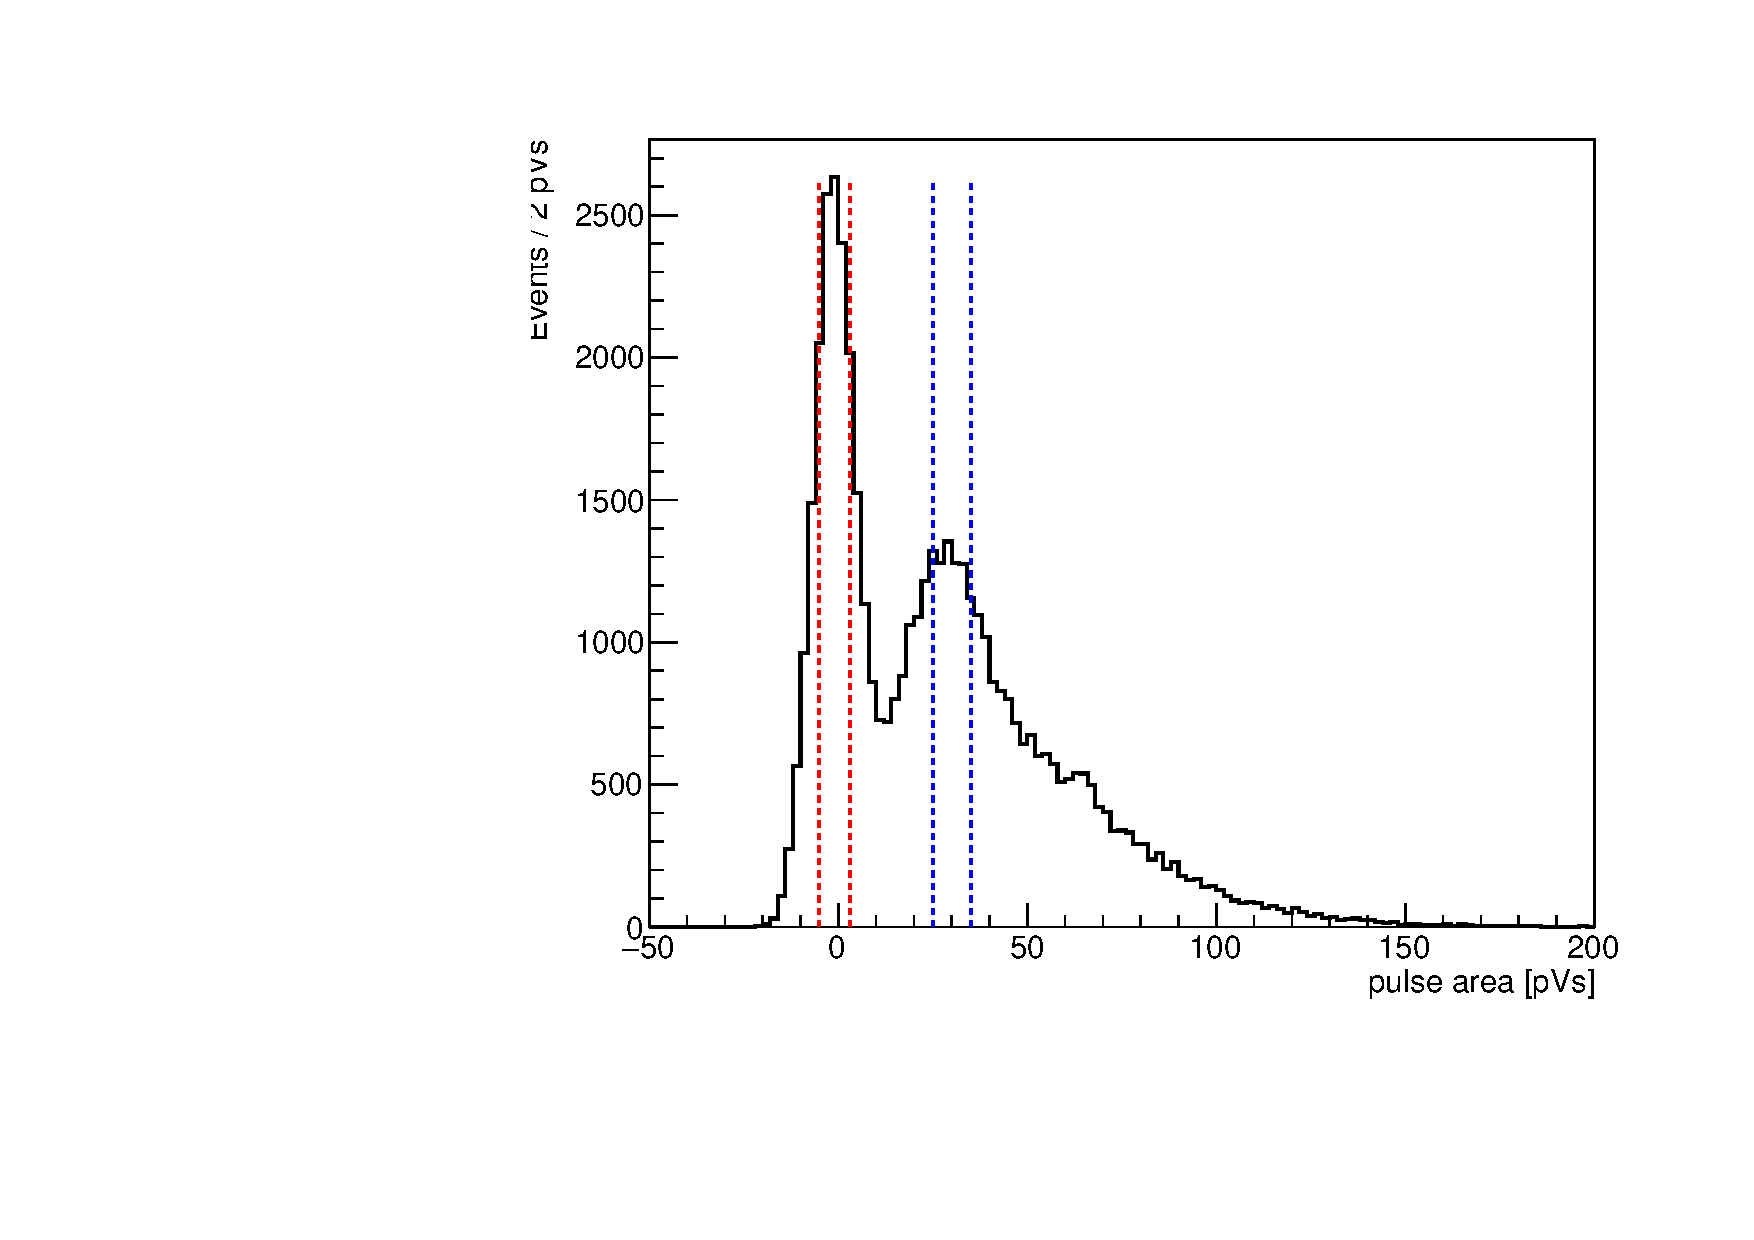
\includegraphics[width=0.375\textwidth]{figs/milliq/pulse_area.pdf}
    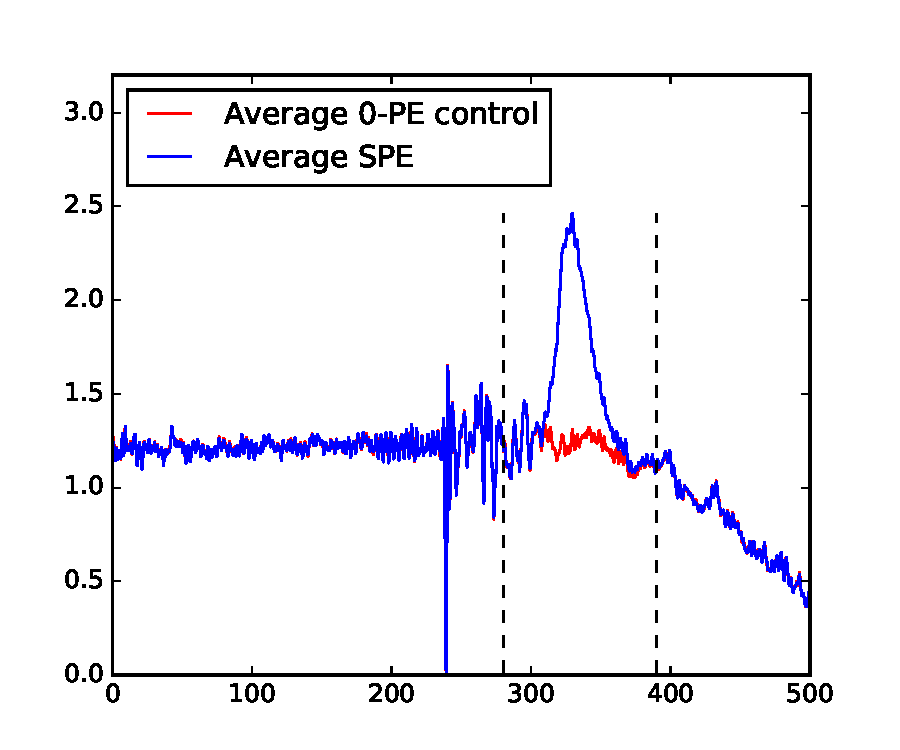
\includegraphics[width=0.375\textwidth]{figs/milliq/avg_spe_control.pdf} \\
    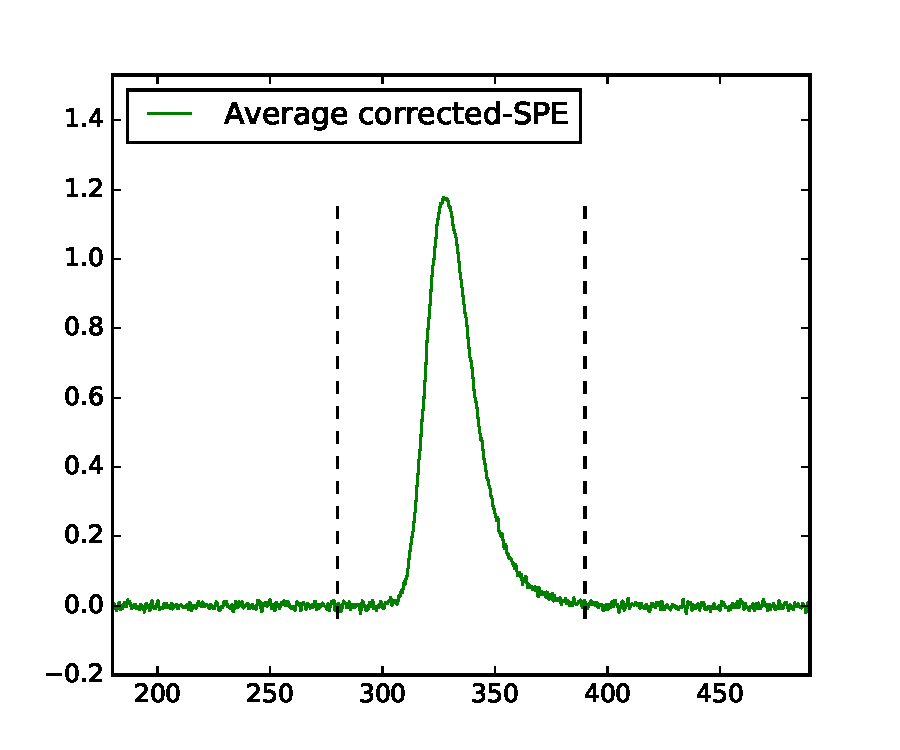
\includegraphics[width=0.375\textwidth]{figs/milliq/avg_spe_fixed.pdf}
    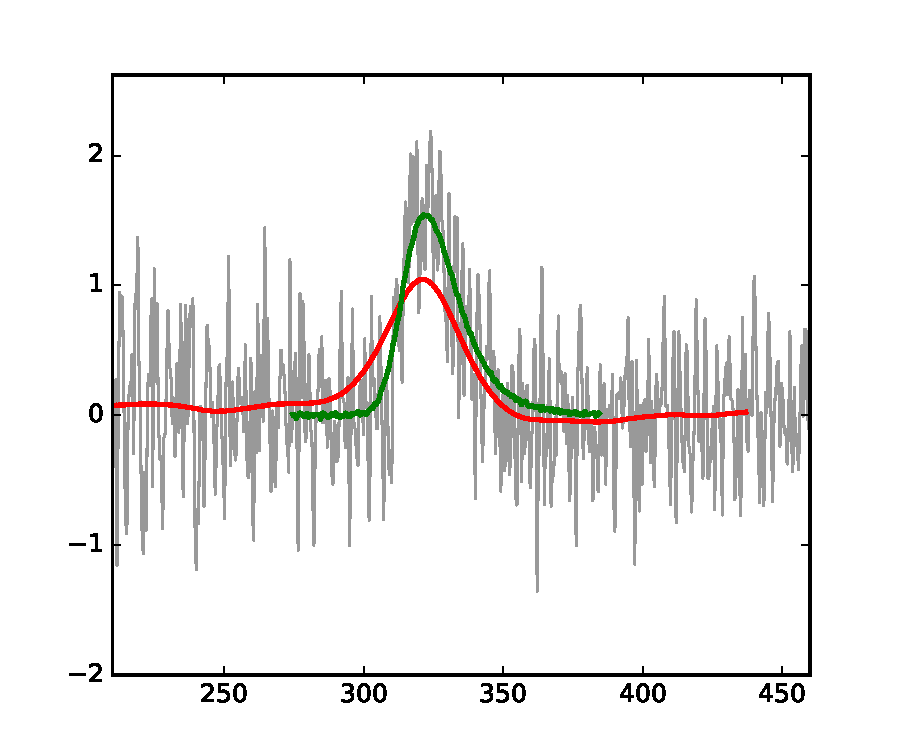
\includegraphics[width=0.375\textwidth]{figs/milliq/samp_smoothed.pdf}
    \caption{Illustration of the procedure for constructing pulse-shape templates,
      in this case for the R878.
      (top left) Area distribution of PMT pulses. Events between the red lines
      are selected for the 0-PE control sample, used to removed fixed electronic noise.
      Events between the blue lines are used as the SPE waveforms.
      (top right) The averaged SPE waveforms (blue) and 0-PE control sample (red).
      (bottom left) The control-subtracted waveform (blue minus red from the top right).
      (bottom right) Illustration of the timing procedure. The red curve is the convolution
      of the raw waveform (gray) with the template (green). The maximum is taken as the pulse time,
      and the SPE waveforms are shifted so that this is aligned before doing the final averaging.
            }
    \label{fig:pulse_shape_proc}
  \end{center}
\end{figure}

\begin{enumerate}\setlength\itemsep{-1mm}
\item Collect a set of waveforms at low enough LED voltage so that $\langle \Npe\rangle\sim 1$.
\item We want to average together many pulses to remove random noise, but there is fixed electronic noise
that is the same in every waveform and does not get averaged away. To remove this, first average together a control
sample of 0-PE events (chosen by selecting events whose pulse area is in the bulk of the 0-PE area distribution).
These events have the same fixed noise but no actual signal.
\item Now, subtract this averaged control waveform from each raw SPE waveform (chosen by selecting events whose pulse
area is near the peak of the SPE area distribution), and average the resulting waveforms together.
This produces a smooth, noise-free template waveform. However, due to small $\mathcal{O}$(5--10 ns) time shifts of individual
pulses, the template is ``smeared'', making it too short and wide.
\item To correct this, modify the above procedure by shifting each control-subtracted SPE waveform in time
so that their peaks line up before averaging.
The time of each pulse is computed by convolving the raw waveform with the non-time-corrected
template from step \#3, and finding the maximum point of this convolution.
\end{enumerate}

This procedure is illustrated in Fig.~\ref{fig:pulse_shape_proc} for the R878, and the resulting templates
for all PMT types are shown in Fig.~\ref{fig:pulse_templates}.

\begin{figure}[t]
  \begin{center}
    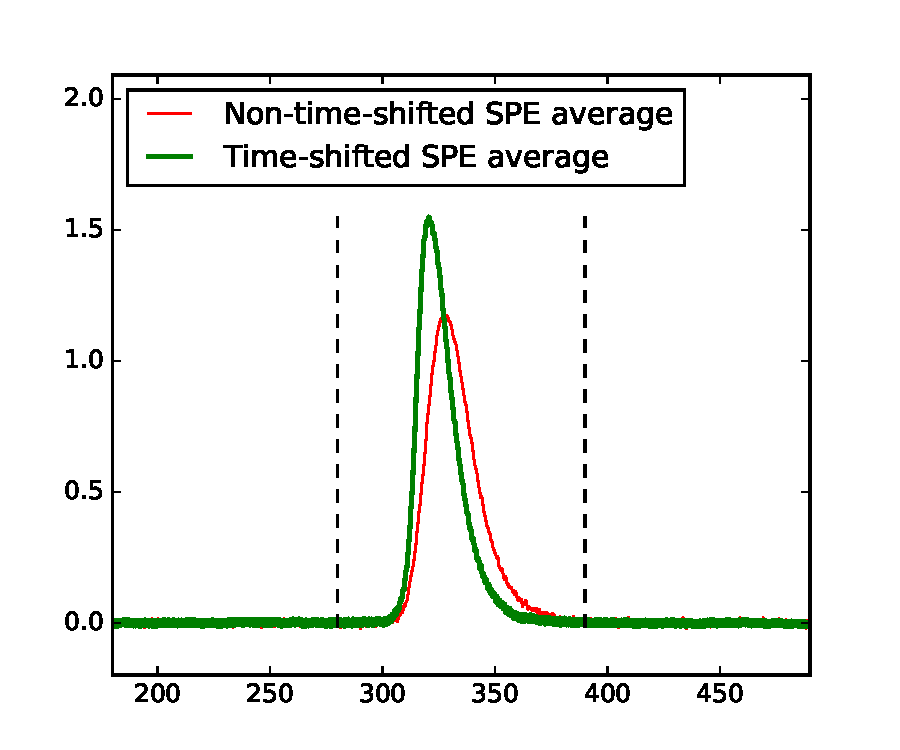
\includegraphics[width=0.325\textwidth]{figs/milliq/avg_spe_fixed_tcorr_878.pdf}
    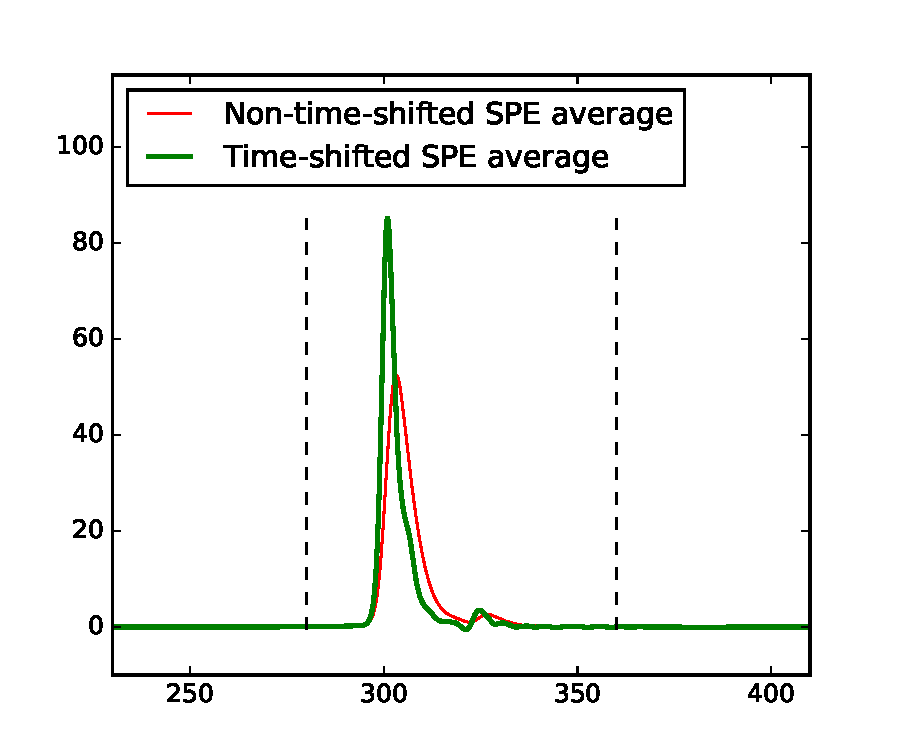
\includegraphics[width=0.325\textwidth]{figs/milliq/avg_spe_fixed_tcorr_7725.pdf}
    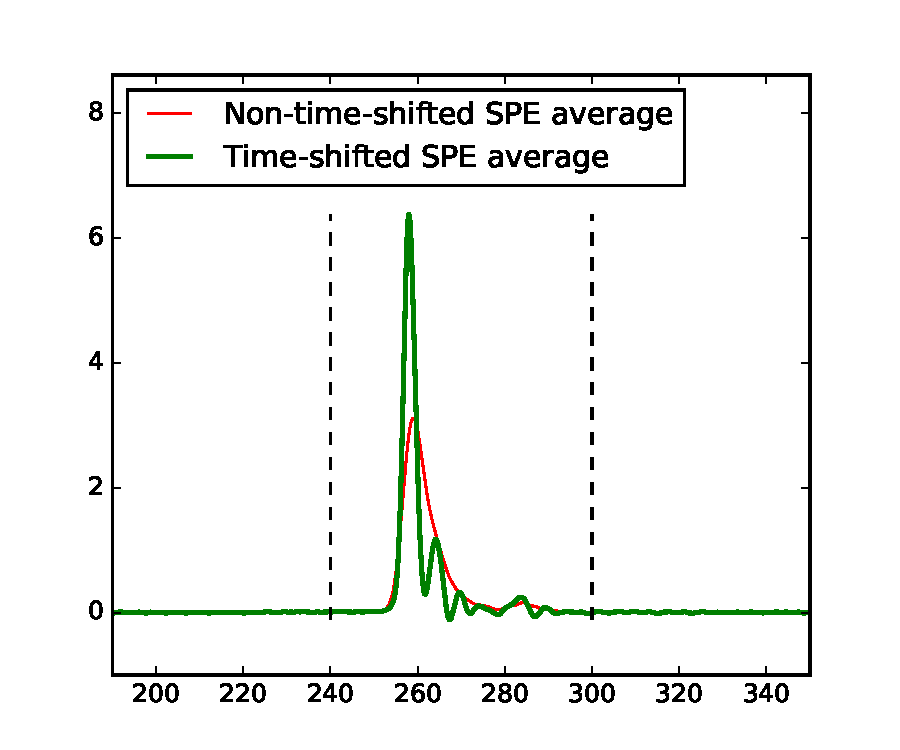
\includegraphics[width=0.325\textwidth]{figs/milliq/avg_spe_fixed_tcorr_ET.pdf}
    \caption{Pulse shape templates derived for the R878 (left), R7725 (center), and ET (right) PMTs. The green curves
      are the time-corrected templates, used for the pulse injection. The red curves are the templates
      before time correction, which are not correct and only shown here for illustration of the effect
      of time shifts.
            }
    \label{fig:pulse_templates}
  \end{center}
\end{figure}

\section{In-situ calibrations}
\label{sec:insitu_calib}
In addition to the LED-based bench calibrations described in the previous section, we also
perform calibrations ``in-situ'' on the installed detector. These can be divided into four
categories, the first two relating to ``pulse size'' and the second two relating to
``pulse timing'':
\begin{itemize}\setlength\itemsep{-1mm}
\item SPE calibration: PMT-dependent characteristic size of a pulse from a single photoelectron
\item \Npe calibration: how many photoelectrons does a particle of a given charge produce in each channel?
\item Channel-dependent timing calibration: per-channel time offsets due to cable lengths, scintillator shape differences, etc.
\item Pulse size-dependent timing calibration: timing differences due to the pulse-finding algorithm responding differently 
to differently sized pulses
\end{itemize}

\subsection{SPE and \Npe calibrations}

First, we measure the mean
pulse area of SPEs. These are expected to differ slightly from the areas measured with the LED
tests, as small magnetic fields and other environmental effects can affect the response of the
PMTs. Second, we perform a ``charge calibration'', or \Npe calibration, 
which measures the number of photoelectrons
generated by a particle of a given charge traveling a given distance through the scintillator.
This measurement is only possible in-situ as it involves properties of the scintillators and
their couplings to the PMTs, in addition to the PMT-specific effects.

The SPE area is measured by selecting PMT afterpulses coming after a pulse from a vertical
cosmic muon. Events are selected in which a top panel and three bars in a vertical line have
hits consistent with a vertically traveling muon. The areas of all secondary pulses are plotted,
and a Gaussian is fit to the peak. The mean of this Gaussian is taken as the peak SPE area for that
channel.

The \Npe calibration is done differently for the slabs, panels, and bars. For the slabs,
events with a throughgoing beam muon are identified, and the peak of the resulting pulse area
distribution in each slab, scaled by the measured mean SPE area, is taken as the \Npe calibration.
For the panels, a similar procedure is used, but with cosmic muons.

\begin{figure}[t]
  \begin{center}
    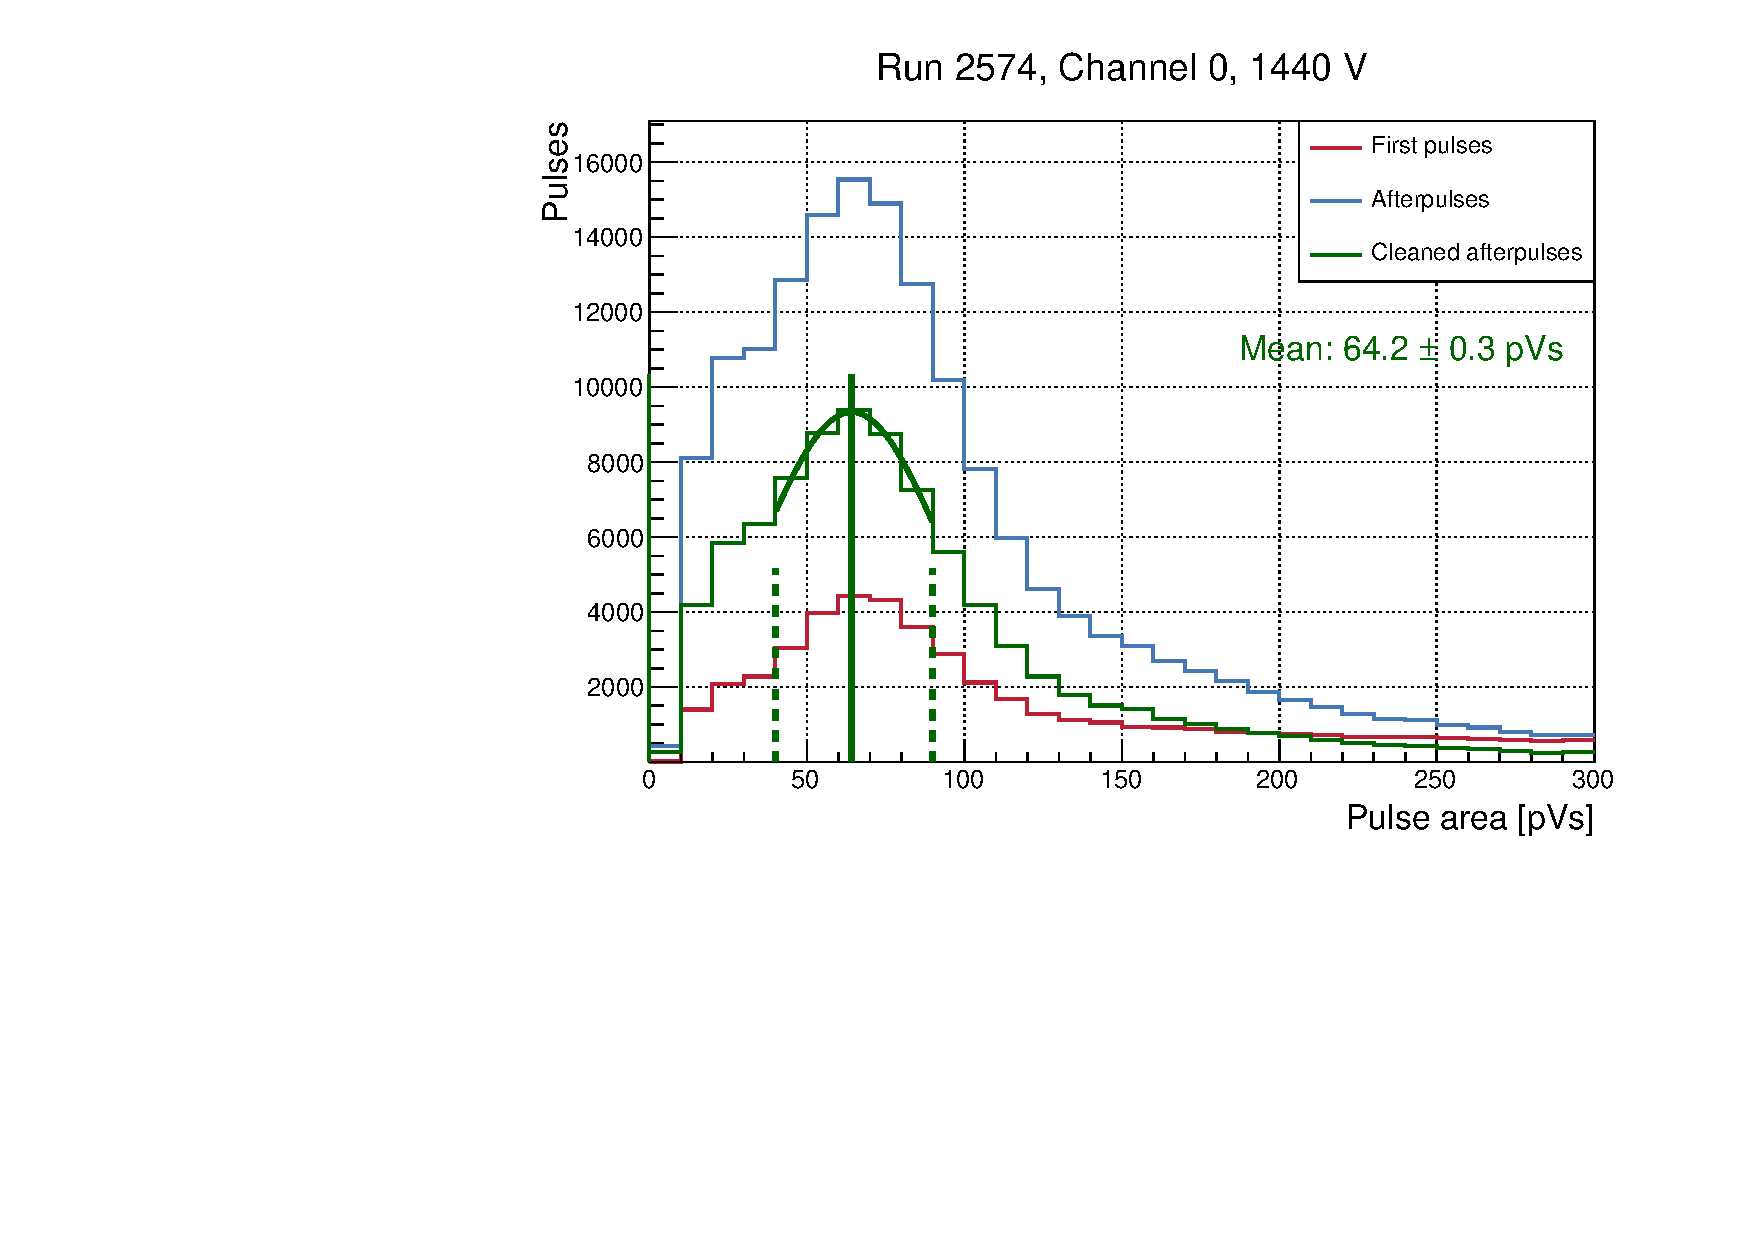
\includegraphics[width=0.475\textwidth]{figs/milliq/spe_area_hist.pdf}
    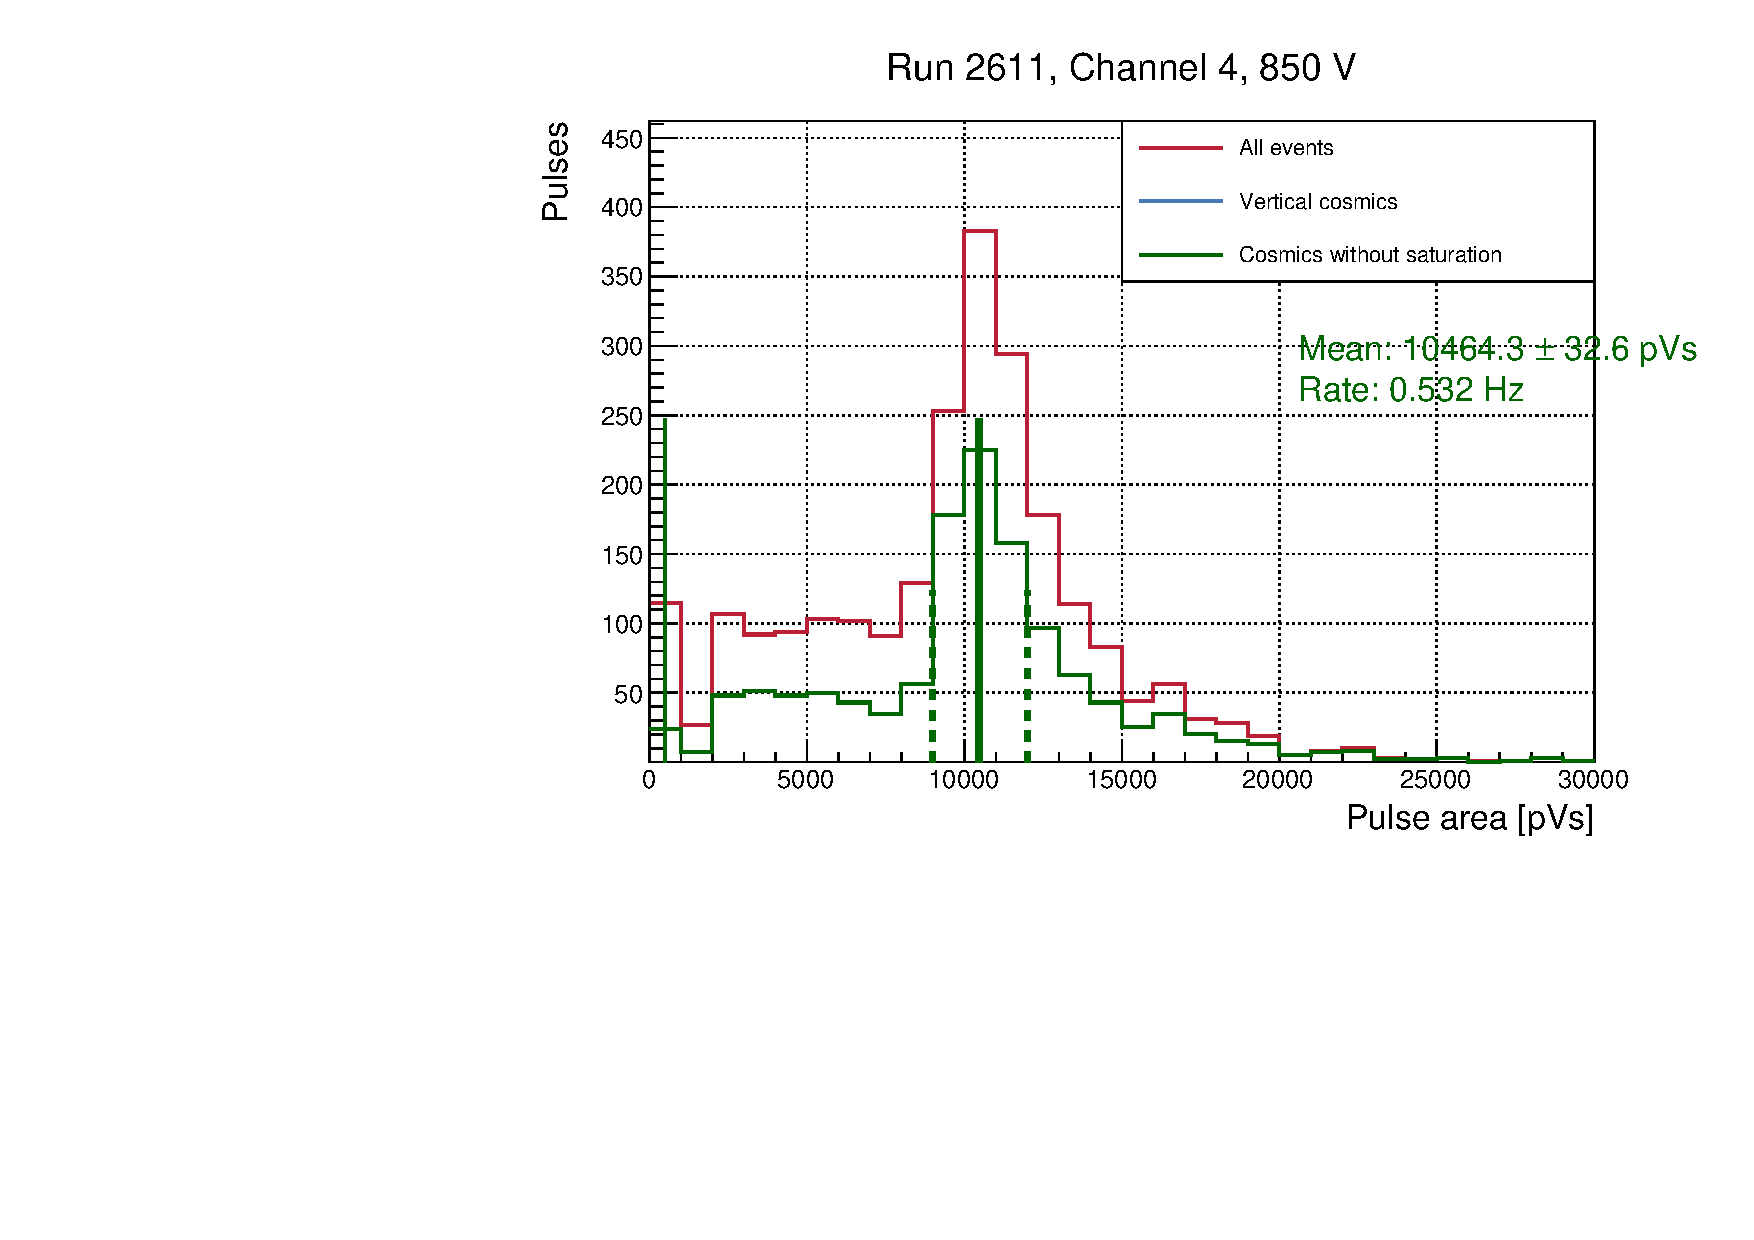
\includegraphics[width=0.475\textwidth]{figs/milliq/cosmic_area_hist.pdf}
    \caption{(left) Example measurement of the mean SPE area of Channel 0 (R878) at 1440 V.
      A selection of cleaned afterpulses is identified (green) and a Gaussian is fit to the peak.
      This measurement is used directly as the SPE calibration, and also as a component of the \Npe calibration.
      (right) An example measurement of the mean cosmic pulse area for Channel 4, at a low HV of 850 V.
            }
    \label{fig:spe_cosmic_area}
  \end{center}
\end{figure}

Performing the \Npe calibration for the bars is more challenging, as the PMTs saturate for
both beam and cosmic muons so a direct measurement is not possible. Instead, an indirect
method, in which pulse areas are extrapolated from lower voltages at which the PMTs do
not saturate, is used. The procedure is as follows:
\begin{enumerate}\setlength\itemsep{-1mm}
\item Measure the mean pulse area for cosmic pulses, at a variety of HVs low enough
that the PMT does not saturate
\item Measure the mean SPE area at 2--3 points near the operating voltage of the PMTs
\item Empirically, the pulse areas scale with HV as a power law function. Jointly fit
power law functions separately to the cosmic and SPE points, with the restriction that
the exponent is the same. Then the ratio between these two functions is the
mean \Npe of a cosmic pulse.
\end{enumerate}

\begin{figure}[htbp]
  \begin{center}
    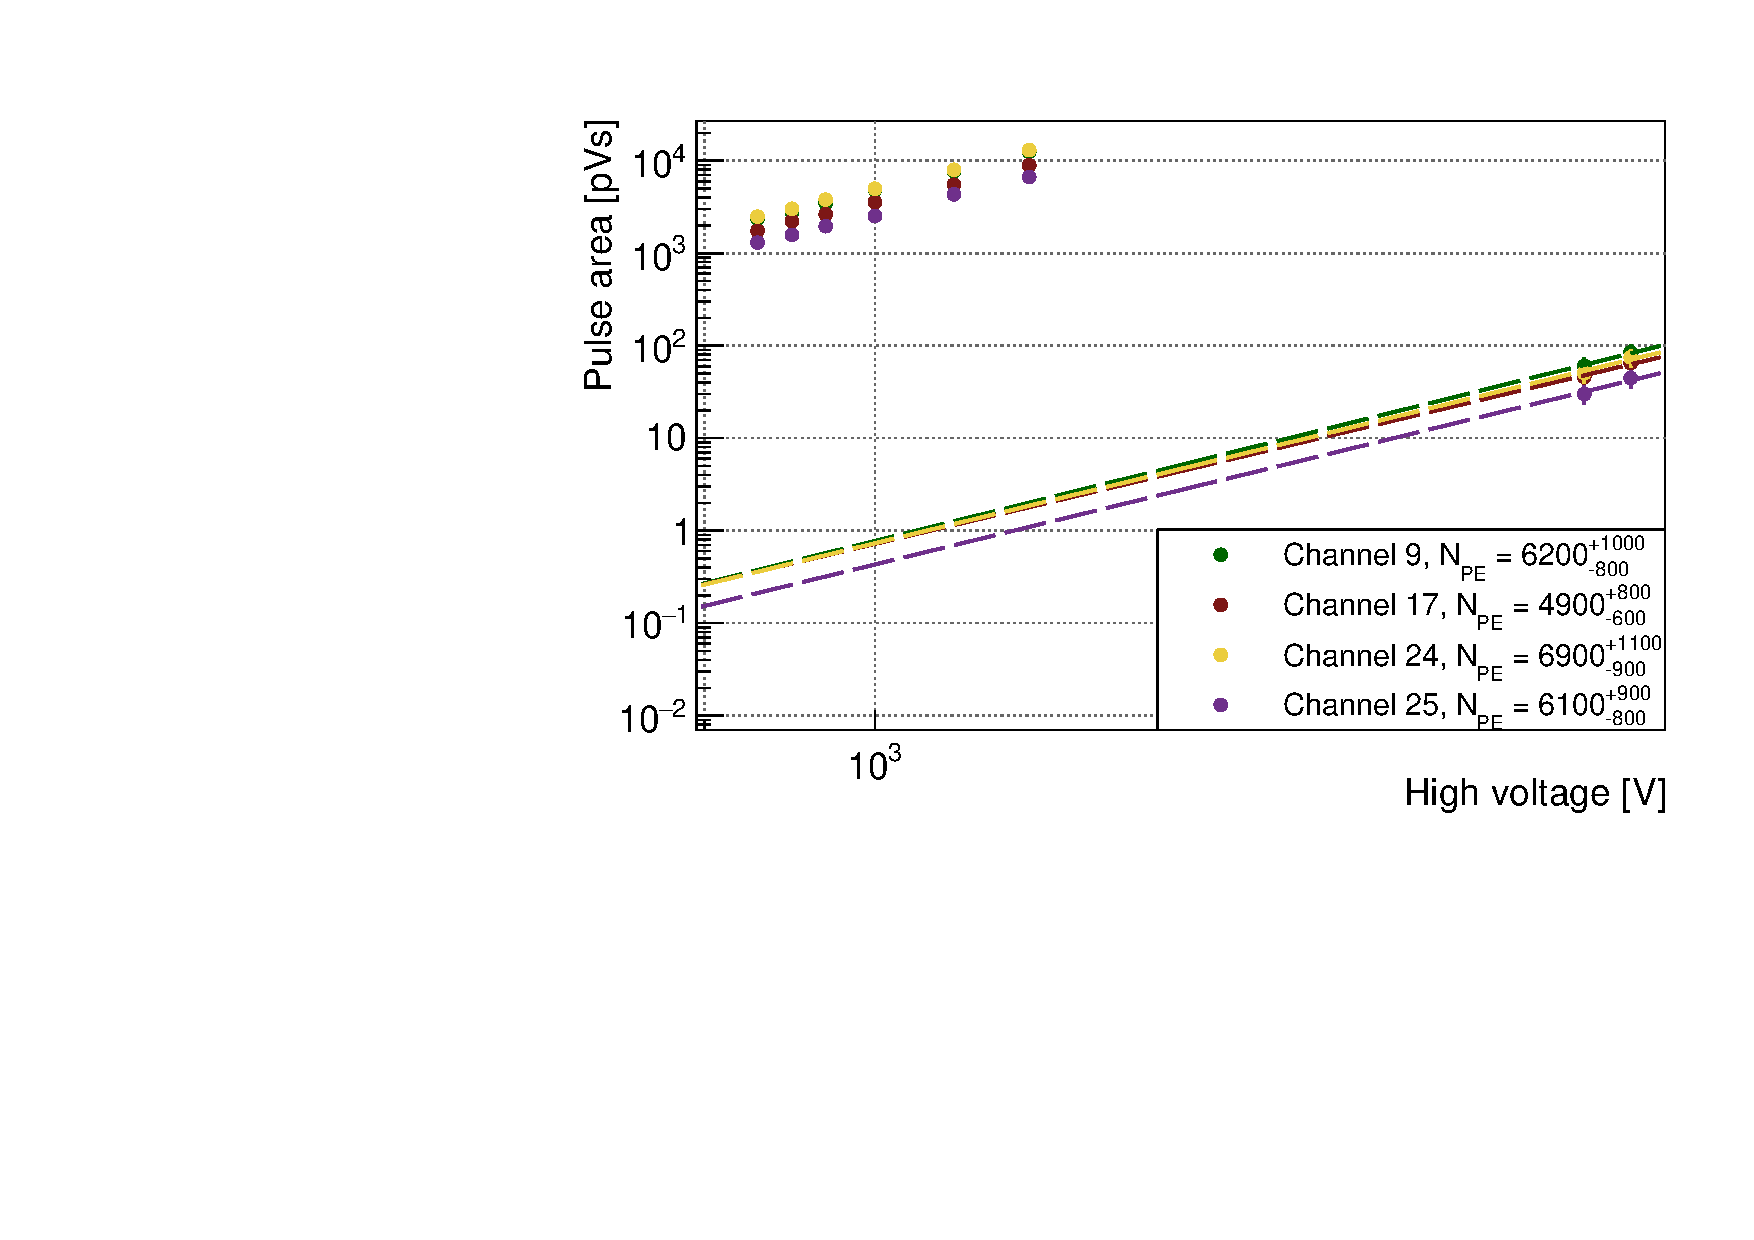
\includegraphics[width=0.675\textwidth]{figs/milliq/npe_calibration_ET.pdf} \\
    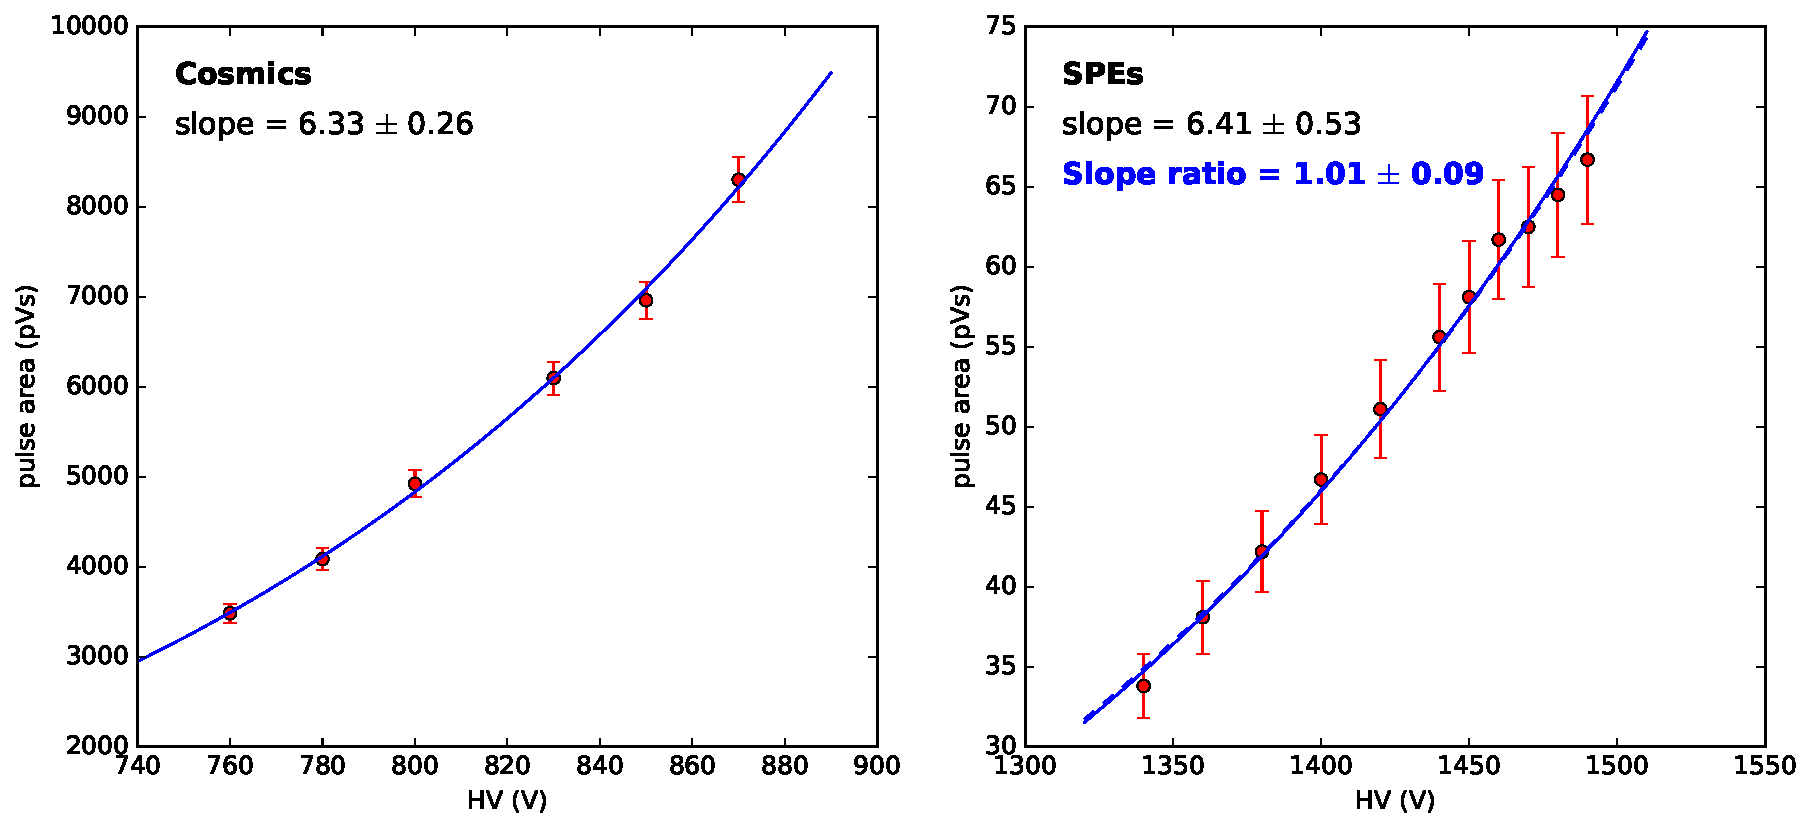
\includegraphics[width=0.775\textwidth]{figs/milliq/npe_calib_slope_comp.pdf}
    \caption{(top) Example \Npe calibration of the four ET channels. The points in the 
      upper left are the measured low-voltage cosmic areas, and the points on the
      right are the mean SPE areas near the operating voltage. Power law functions
      are jointly fit to the cosmic and SPE points, with the restriction that the exponent
      is the same; these fits are shown as dashed lines through the SPE points. The ratio
      of the two fits is taken as the \Npe calibration.
      (bottom) A validation of the procedure for Channel 1. A key assumption of the method is
      that the power law exponents are the same for the cosmic and SPE points. Here, we fit each set
      separately and find that the exponent ratio is $1.01\pm0.09$.
            }
    \label{fig:npe_calibration}
  \end{center}
\end{figure}

Example measurements of the mean SPE and cosmic pulse areas are shown in Fig.~\ref{fig:spe_cosmic_area}.
The \Npe calibration procedure is illustrated in Fig.~\ref{fig:npe_calibration}. The top plot
shows the measured cosmic (upper left) and SPE (middle right) areas, and the dashed lines
show the fitted power law function through the SPE points. The bottom plots show an example validation
of the procedure; on the left is a fit to the cosmic points, and on the right is an independent fit
to a number of SPE points at higher voltages. The ratio of the fitted exponents
is $1.01\pm0.09$, showing that the fit is consistent between the two sets of points as assumed.
This is done independently for each channel; good agreement is seen in all cases.


\subsection{Timing calibrations}
A throughgoing particle will leave pulses at different times in different channels,
due to time-of-flight, scintillator shape differences, varying cable lengths,
and other effects. We calibrate these differences away such that a beam-based
throughgoing particle traveling at the speed of light is expected to generate
a pulse at the same time in each channel. This is done as follows:
\begin{enumerate}\setlength\itemsep{-1mm}
\item Calibrate bars within each ``slice'' (left/right side of each layer),
by tagging vertical cosmics that hit the top pannel and each bar in the slice.
The mean cosmic pulse time is taken as the calibration.
\item Calibrate the two slices in each layer, by tagging cosmics that
hit the top panel and at least one bar in each slice.
\item Calibrate the slabs by tagging beam-based muons passing through
all four slabs.
\item Calibrate each layer by tagging beam-based muons and comparing
to the time in the nearest slab.
\item Calibrate the panels by tagging cosmics that hit a panel
and at least one bar in the same layer as the panel.
\end{enumerate}

A validation of this procedure is shown in Fig.~\ref{fig:mq_time_calib}, in which
the calibrated time difference between bar pulses in layer 3 and layer 1 for muon events
is plotted. There is a single Gaussian distribution centered at 0 ns for beam 
muons, as expected if the calibration is done correctly.

\begin{figure}[t]
  \begin{center}
    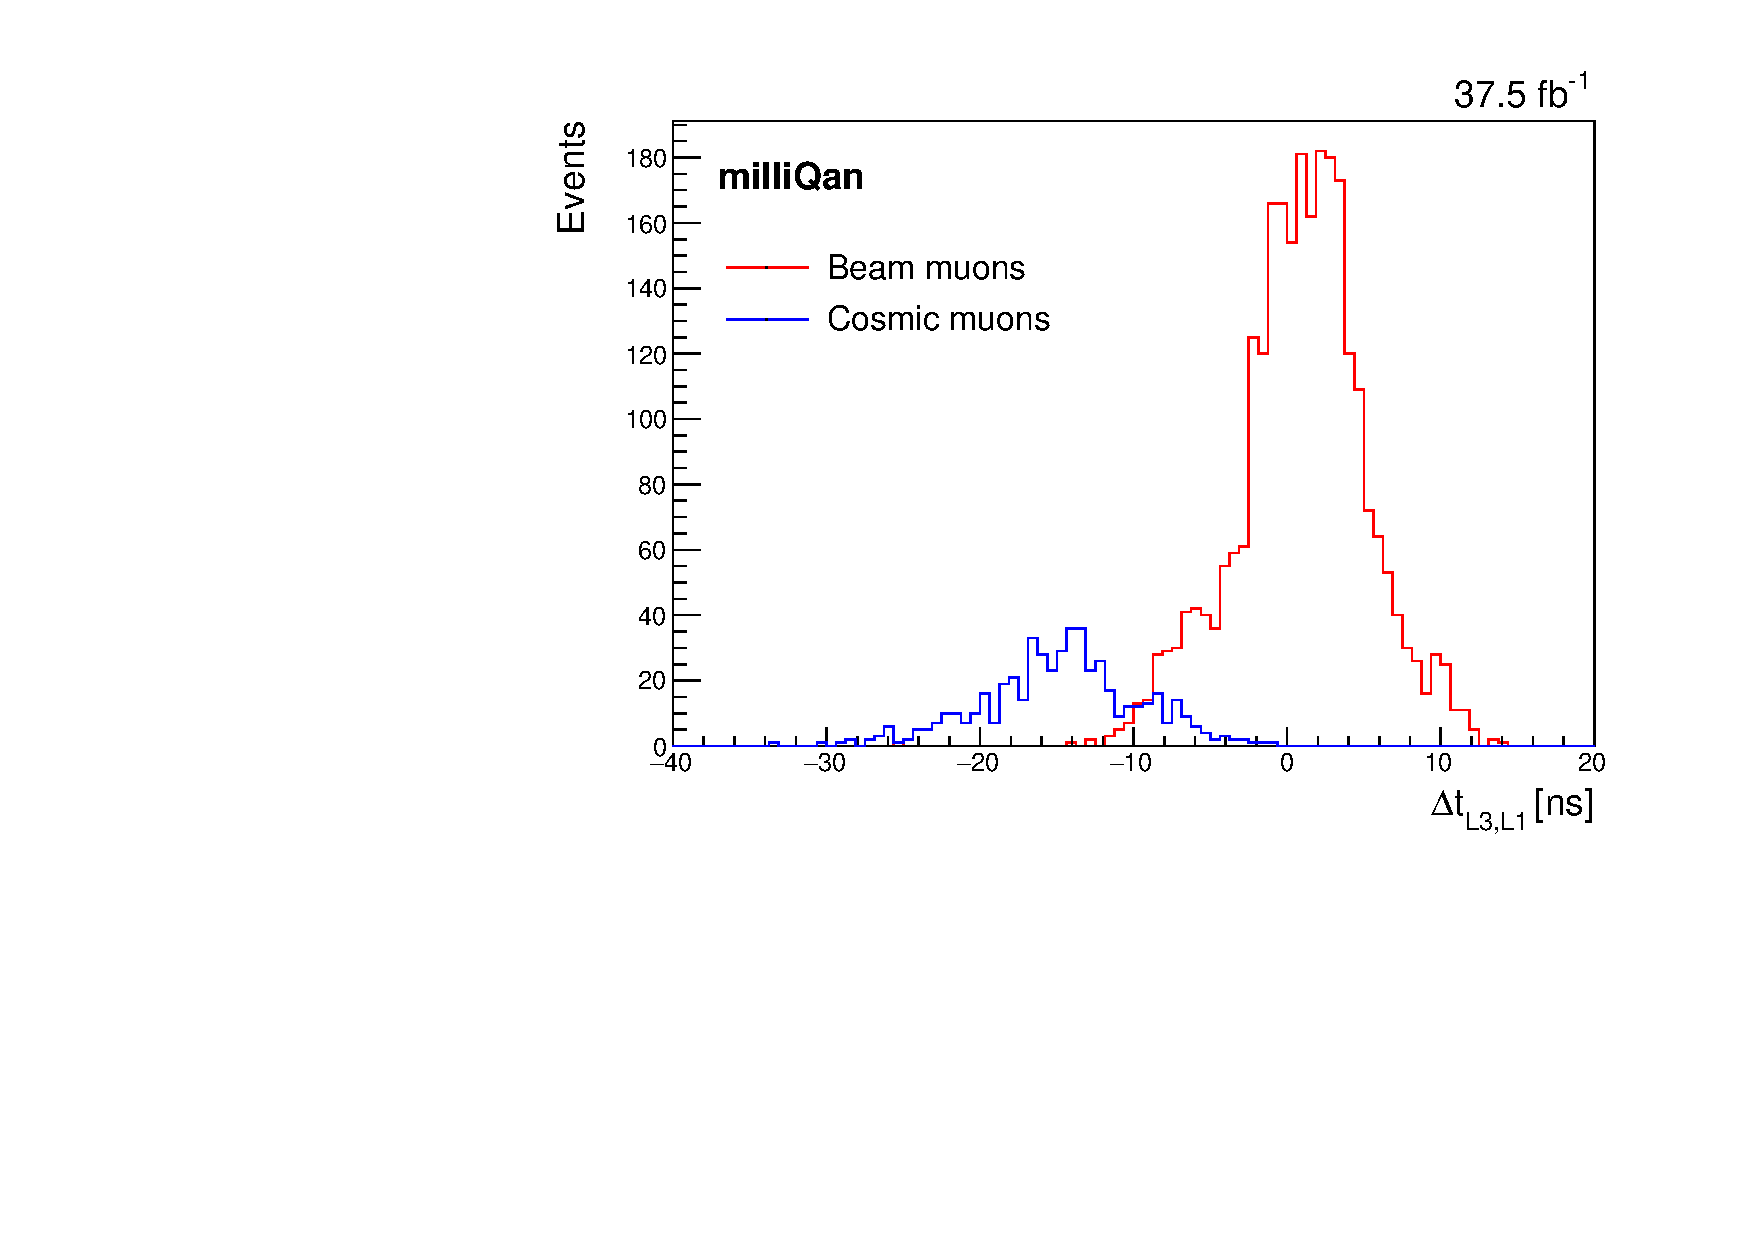
\includegraphics[width=0.60\textwidth]{figs/milliq/time_calib.pdf}
    \caption{Calibrated time difference between the bar pulses in layer 3 and layer 1,
      for events in which a muon is tagged in all four slabs and bars in all
      three layers. Cosmic and beam muons are distinguished based on the time difference
      in the first and fourth slabs. The beam muon distribution is centered at 0 ns as expected,
      and has a resolution of $\sim$5 ns. The cosmic distribution is centered at 15 ns,
      exactly as expected from time-of-flight considerations ($\Delta t=2\times 2.2\text{ m}/c = 15$ ns).
            }
    \label{fig:mq_time_calib}
  \end{center}
\end{figure}

In addition to the overall channel-dependent time calibrations, we also correct for the known effect
of ``time walk'', in which small pulses are reconstructed at later times than large pulses. This is
due to the algorithm for computing pulse time, which finds the time at which a signal rises above
some fixed voltage threshold. Large pulses rise quicker than small pulses, and are hence assigned earlier
times. This phenomenon is illustrated in Fig.~\ref{fig:mq_time_walk}, in which we plot the pulse
size vs. time delay for pulses in bars neighboring a tagged throughgoing muon (likely caused by
showering from the muon). One observes a distinct trend in time as the pulse size is varied.

\begin{figure}[t] 
  \begin{center}
    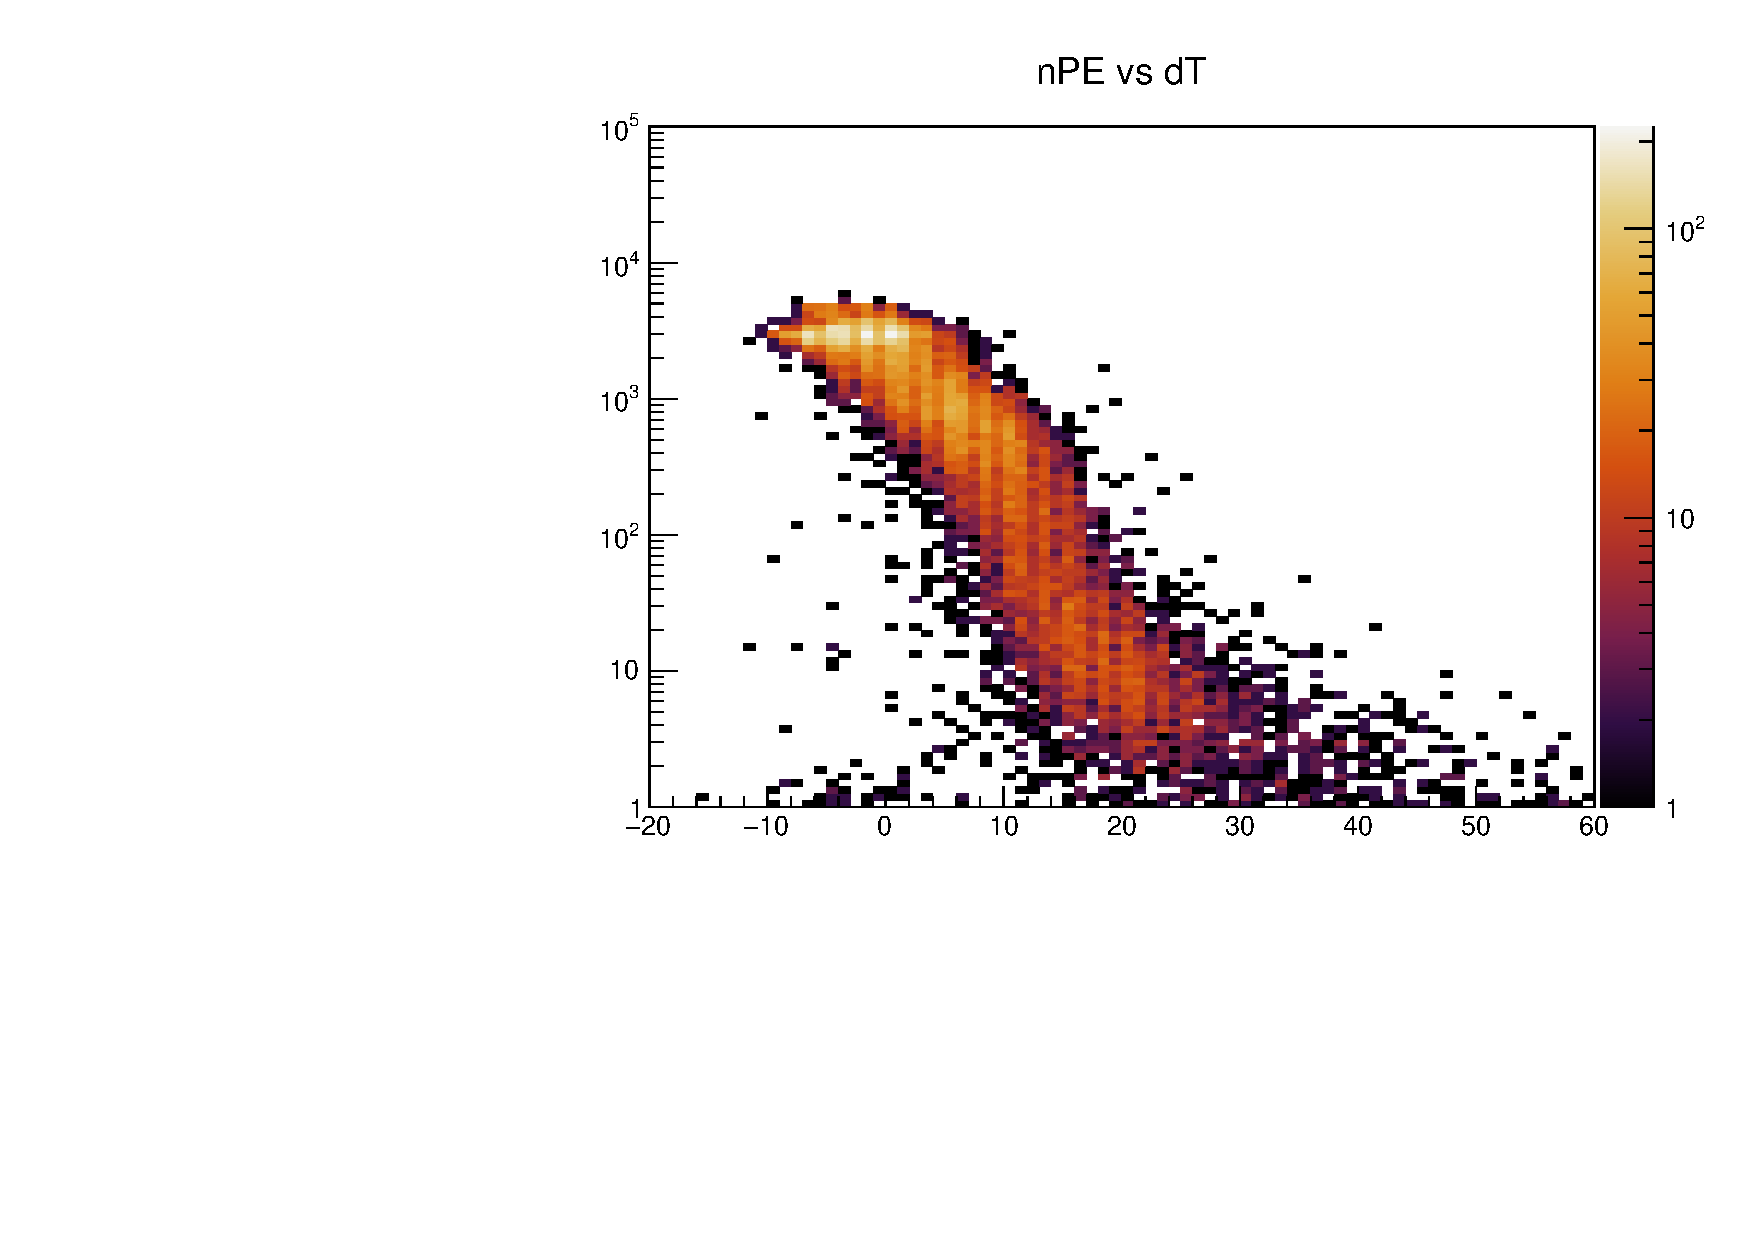
\includegraphics[width=0.48\textwidth]{figs/milliq/npe_vs_dt_878.pdf}
    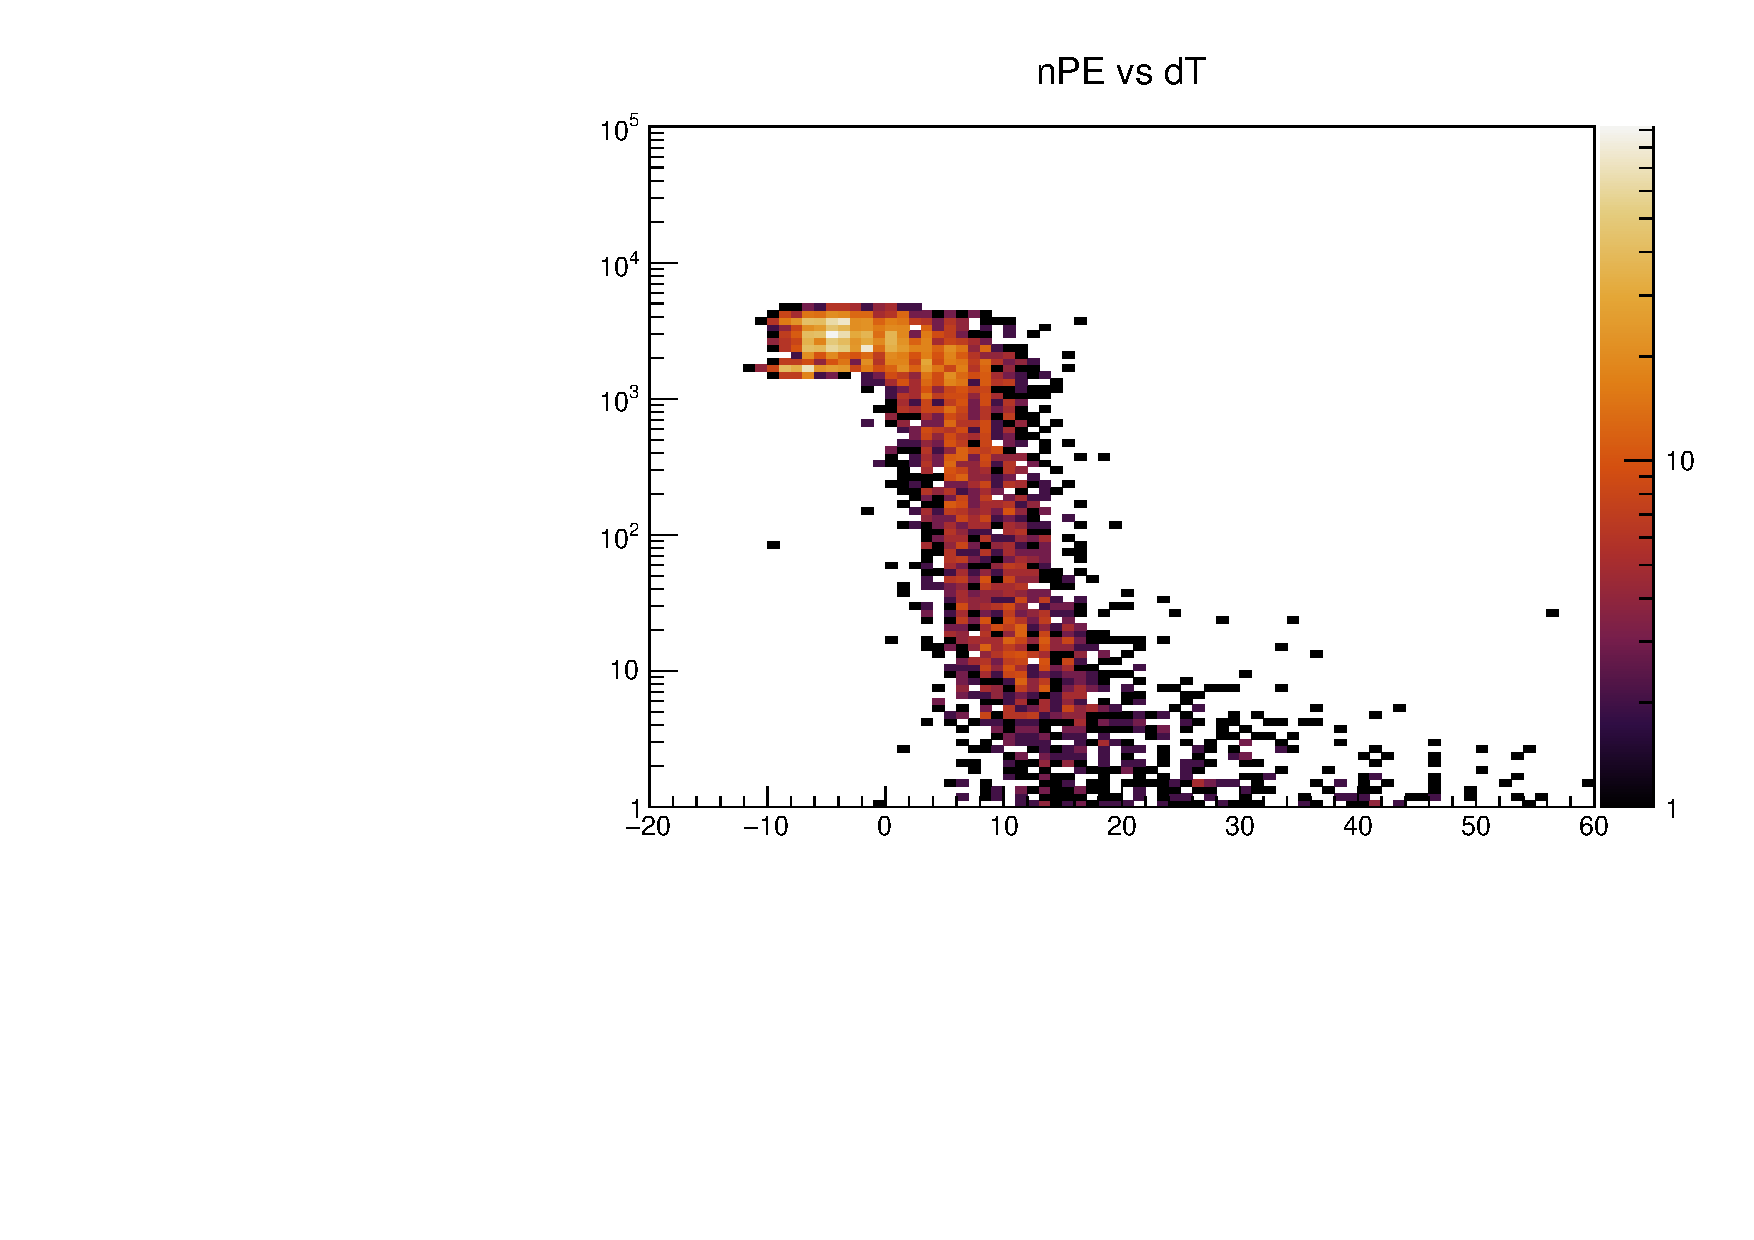
\includegraphics[width=0.48\textwidth]{figs/milliq/npe_vs_dt_ET.pdf}
    \caption{Pulse size in terms of \Npe ($y$ axis) vs. time delay in ns ($x$ axis),
      for R878s (left) and ETs (right). We tag events in which a beam muon 
      passes through all four slabs and three bars in a straight line, and use pulses
      in neighboring bars caused by e.g. showering from the muon. Time delay is relative
      to the time in the preceding slab. One observes a delay of up to $\sim$20 ns
      between pulses of different sizes. The effect is more pronounced in the R878.
            }
    \label{fig:mq_time_walk}
  \end{center}
\end{figure}

The mean delay as a function of pulse size is extracted in bins of pulse area, and this is used
to correct individual pulse times. This is done separately for each PMT species, as the effect
highly depends on the specific pulse shape. Further, there are slight differences in the size
of the effect between data and simulation, so separate calibrations are derived.

Finally, we also observe that the resolution (i.e. the spread in time for a given pulse size
in Fig.~\ref{fig:mq_time_walk}) is slightly worse in data than in simulation. To account for 
this, we smear the reconstructed pulse times in simulation by an area-dependent factor such
that the time resolutions match those measured in data.

\section{Monte Carlo generation}
\label{sec:mq_mcgen}
Any process at the LHC that produces an $e^+e^-$ pair via a virtual
photon can also produce a $\zeta^+\zeta^-$ pair (we use $\zeta$ as the symbol for an mCP).
This includes the direct vector meson decays $V\to e^+e^-$, where 
$V=\rho,\;\omega,\;\phi,\;\psi,\;\text{or}\;\Upsilon$,
the Dalitz decays $A\to e^+e^-\gamma$, where
$A=\pi^0,\;\eta,\;\text{or}\;\eta'$, and the Dalitz decays 
$\omega\to e^+e^-\pi^0$ and $\eta'\to e^+e^-\omega$.
Additionally, $\zeta^+\zeta^-$ pairs can be produced via
the Drell-Yan process, as with couplings to the photon and
$Z$ of $\varepsilon e$ and $\varepsilon e\tan\theta_w$, respectively.

We generate Drell-Yan decays with \textsc{Madgraph}~\cite{madgraph}, using the
Lagrangian~\ref{eq:mcp_lagr}, with a cut on the invariant mass of the $\zeta^+\zeta^-$
pair of 2\GeV. The Drell-Yan production mode is subdominant when the mass of the mCP
is below half the $\Upsilon$ mass, around 5\GeV.

For mCP pairs produced through meson decay, we perform the two-body/Dalitz decays
manually and store the resulting mCP four-vectors. This requires two pieces of
information for each process: (1) the branching ratio of the meson
to a $\zeta^+\zeta^-$ pair (for Dalitz decays, we need the \textit{differential}
width as a function of the $\zeta^+\zeta^-$ invariant mass), and (2)
the differential cross sections to produce the parent meson as a function of \pt and $\eta$..

Branching ratios for direct vector meson decays can be computed by simply
scaling the $e^+e^-$ BR by a phase space factor:
\be
\frac{\Gamma(V\to\zeta^+\zeta^-)}{\Gamma(V\to e^+e^-)} = 
(Q/e)^2\frac{(1-4x_\zeta^2)^{1/2}(1+2x_\zeta^2)}{(1-4x_e^2)^{1/2}(1+2x_e^2)},
\ee
where $x_*=m_*/m_V$ (this comes from the Van Royen-Weisskopf formula~\cite{vanroyen}).

For Dalitz decays $A\to\zeta^+\zeta^-X$, we can write the differential width as a function of the $\zeta^+\zeta^-$
invariant mass as~\cite{landsberg}
\be
\begin{split}
\frac{d\Gamma}{dq^2} = &\frac{C\alpha}{3\pi q^2} \left(1+\frac{2m_\zeta^2}{q^2}\right)
\sqrt{1-\frac{4m_\zeta^2}{q^2}} \\
&\left[\left(1+\frac{q^2}{m_A^2-m_X^2}\right)-\frac{4m_A^2q^2}{(m_A^2-m_X^2)^2}\right]^{3/2}
\;|F(q^2)|^2 \;\;\Gamma(A\to X\gamma),
\end{split}
\ee
where $q^2$ is the invariant mass of the $\zeta^+\zeta^-$ pair, $C$ is 2 if
$X$ is a $\gamma$ otherwise 1, and $F(q^2)$ is a form factor that can be approximated
in the Vector Dominance Model as
\be
|F(q^2)|^2 = \frac{m_\rho^4+m_\rho^2\Gamma_\rho^2}{(m_\rho^2-q^2)^2+m_\rho^2\Gamma_\rho^2},
\ee
where $m_\rho$ and $\Gamma_\rho$ are the mass and total width of the $\rho$ meson.

Cross sections for the production of parent mesons are acquired in a variety of ways.
For direct~\cite{yqma:jpsi} and 
$B$ meson-mediated~\cite{fonll} production of J/$\psi$
and $\psi'$ mesons, cross sections and \pt distributions (including uncertainties)
are taken directly from theory calculations. Theoretical calculations of $\Upsilon$
production are not reliable at low \pt, so we use differential cross sections
measured by experiment. For $\pt>20\GeV$, we use cross sections measured
at $\sqrt{s}=13\TeV$~\cite{Sirunyan:2017qdw}, and at lower \pt we use measurements
from 7\TeV~\cite{Aad:2012dlq}, rescaled using the measured ration of 13 to 7\TeV cross sections
at slightly higher rapidity.

Differential cross sections for all light-flavor mesons except $\phi$ mesons
are computed by generating minimum bias events in \textsc{pythia8}~\cite{pythia},
with the Monash 2013 tune~\cite{Skands:2014pea}. This is the tune that gives
best agreement with several measurements of light meson rates and \pt spectra
at the LHC~\cite{ALICE-PUBLIC-2018-004,Acharya:2018qnp,Acharya:2017tlv,Sirunyan:2017zmn}, 
albeit in most cases at a center of mass energies lower than 13\TeV.
The MC spectra for $\eta\;(\rho,\omega)$ with $\pt<3\;(1)\GeV$ are scaled
down by factors as large as two, based on these experimental comparisons.
$\phi$ production is modeled with the \textsc{pythia6} generator~\cite{pythia6}
using the DW tune~\cite{Albrow:2006rt}, since this MC setup best reproduces
$\phi$ meson data~\cite{Aad:2014rca}. All \textsc{pythia} minimum bias MC is normalized
to a total inelastic $pp$ cross section of $80\pm10$ mb based on a measurement
by ATLAS~\cite{ATLAS:ppxsec} (with additional uncertainty to account for slight disagreement
between experimental measurements). An additional 30\% uncertainty, uncorrelated
between production modes, is assessed on the total cross sections to 
account for the modeling of meson rates per minimum bias event.

\begin{figure}[t]
  \begin{center}
    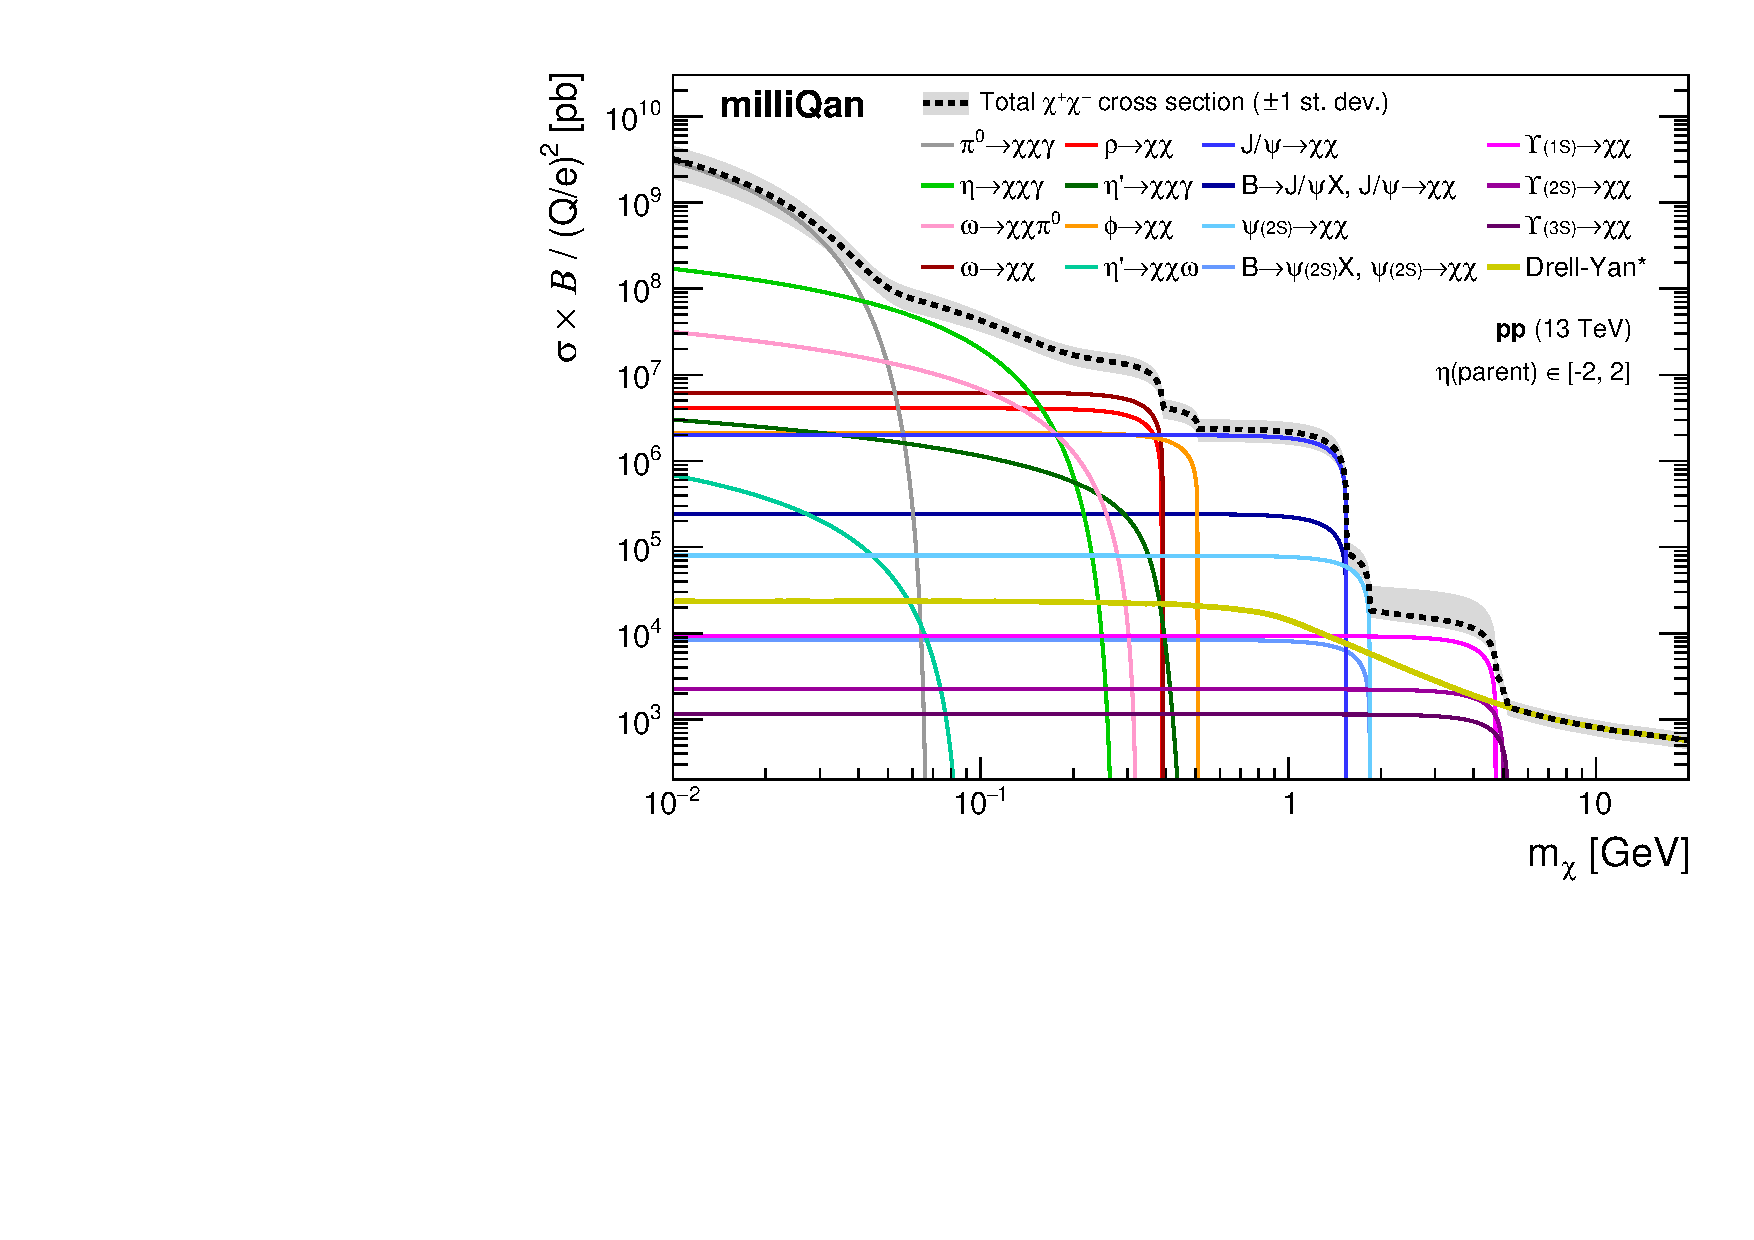
\includegraphics[width=0.80\textwidth]{figs/milliq/mcp-xsec.pdf}
    \caption{Cross section times branching ratio values for all considered
      production modes of $\zeta^+\zeta^-$ pairs, normalized to a charge
      of $Q/e=1$. For non-DY modes, the mother particle must be
      within $|\eta|<2$ (though the $\zeta^\pm$ may have $|\eta|>2$).
      For DY, the plotted cross section requires at least one mCP
      to have $|\eta|<1$. The plateau in DY cross section below 
      $m_\zeta=1\GeV$ is due to a 2\GeV $\zeta^+\zeta^-$ invariant
      mass cut in \textsc{Madgraph}. The gray band on the total
      cross section represents the total theoretical uncertainty
      in the cross section, adding in quadrature the uncertainties
      on each individual mode (with the exception of the 12.5\%
      $pp$ inelastic cross section uncertainty, which is correlated
      across all relevant modes).
            }
    \label{fig:mcp_xsec}
  \end{center}
\end{figure}

A plot summarizing the cross section times branching ratio values
for all $\zeta^+\zeta^-$ production modes is shown in Fig.~\ref{fig:mcp_xsec}.
At low masses, production is dominated by Dalitz decays of light mesons
$\pi^0$, $\eta$. At around a few hundred \MeV, direct decays
of $\omega$'s and $\rho$'s dominate. Near 1\GeV, J/$\psi$'s provide
almost all of the cross section, before the rate falls off substantially
past half the J/$\psi$ mass near 1.5\GeV. $\Upsilon$'s become the dominant
production mode until they fall off at 5\GeV, after which
only Drell-Yan contributes. Note that if this plot were continued,
the rate would drop substantially again near half the $Z$ mass at
roughly 45\GeV.

In addition to mCPs, we are also interested in simulating both beam-based and
cosmic muons in order to compare to data and calibrate/validate the simulation.
Four beam-based muon production modes are considered: heavy-flavor (b or c) meson
decays, light-flavor meson (usually $\pi^\pm$ or $K^\pm$) and tau decays, $W$ boson decays, and $Z$ boson decays.
Differential cross sections for muons from heavy-flavor meson decay are taken from
the FONLL tool~\cite{fonll} (the same that is used for $B\to\psi X$ decays for mCP
generation). The overall $b\bar{b}$ cross section produced by this tool is
known to be low based on a measurement from CMS~\cite{CMS:bhadron}, so the total
rate is scaled up by a factor of $1.25\pm0.25$.
Differential cross sections for light-flavor meson and tau decay are taken from
\textsc{pythia8} MinBias generation with the CUETP8M1 tune. Rates from $W$ and $Z$ decay
are taken from \textsc{Madgraph}.

The composition and \pt distribution of muons that make it to the milliQan detector
face (after the propagation described shortly) are shown in Fig.~\ref{fig:mq_muon_ptdist}.
Only muons with $\pt\gtrsim15\GeV$ make it to the detector, as lower-energy muons
are stopped short, either in CMS or the rock. Of the muons that do make it to milliQan,
53\% are from b hadrons, 29\% are from c hadrons, 14\% are from light-flavor mesons
or taus, 3\% are from $W$ bosons, and 1\% are from $Z$ bosons.

\begin{figure}[t]
  \begin{center}
    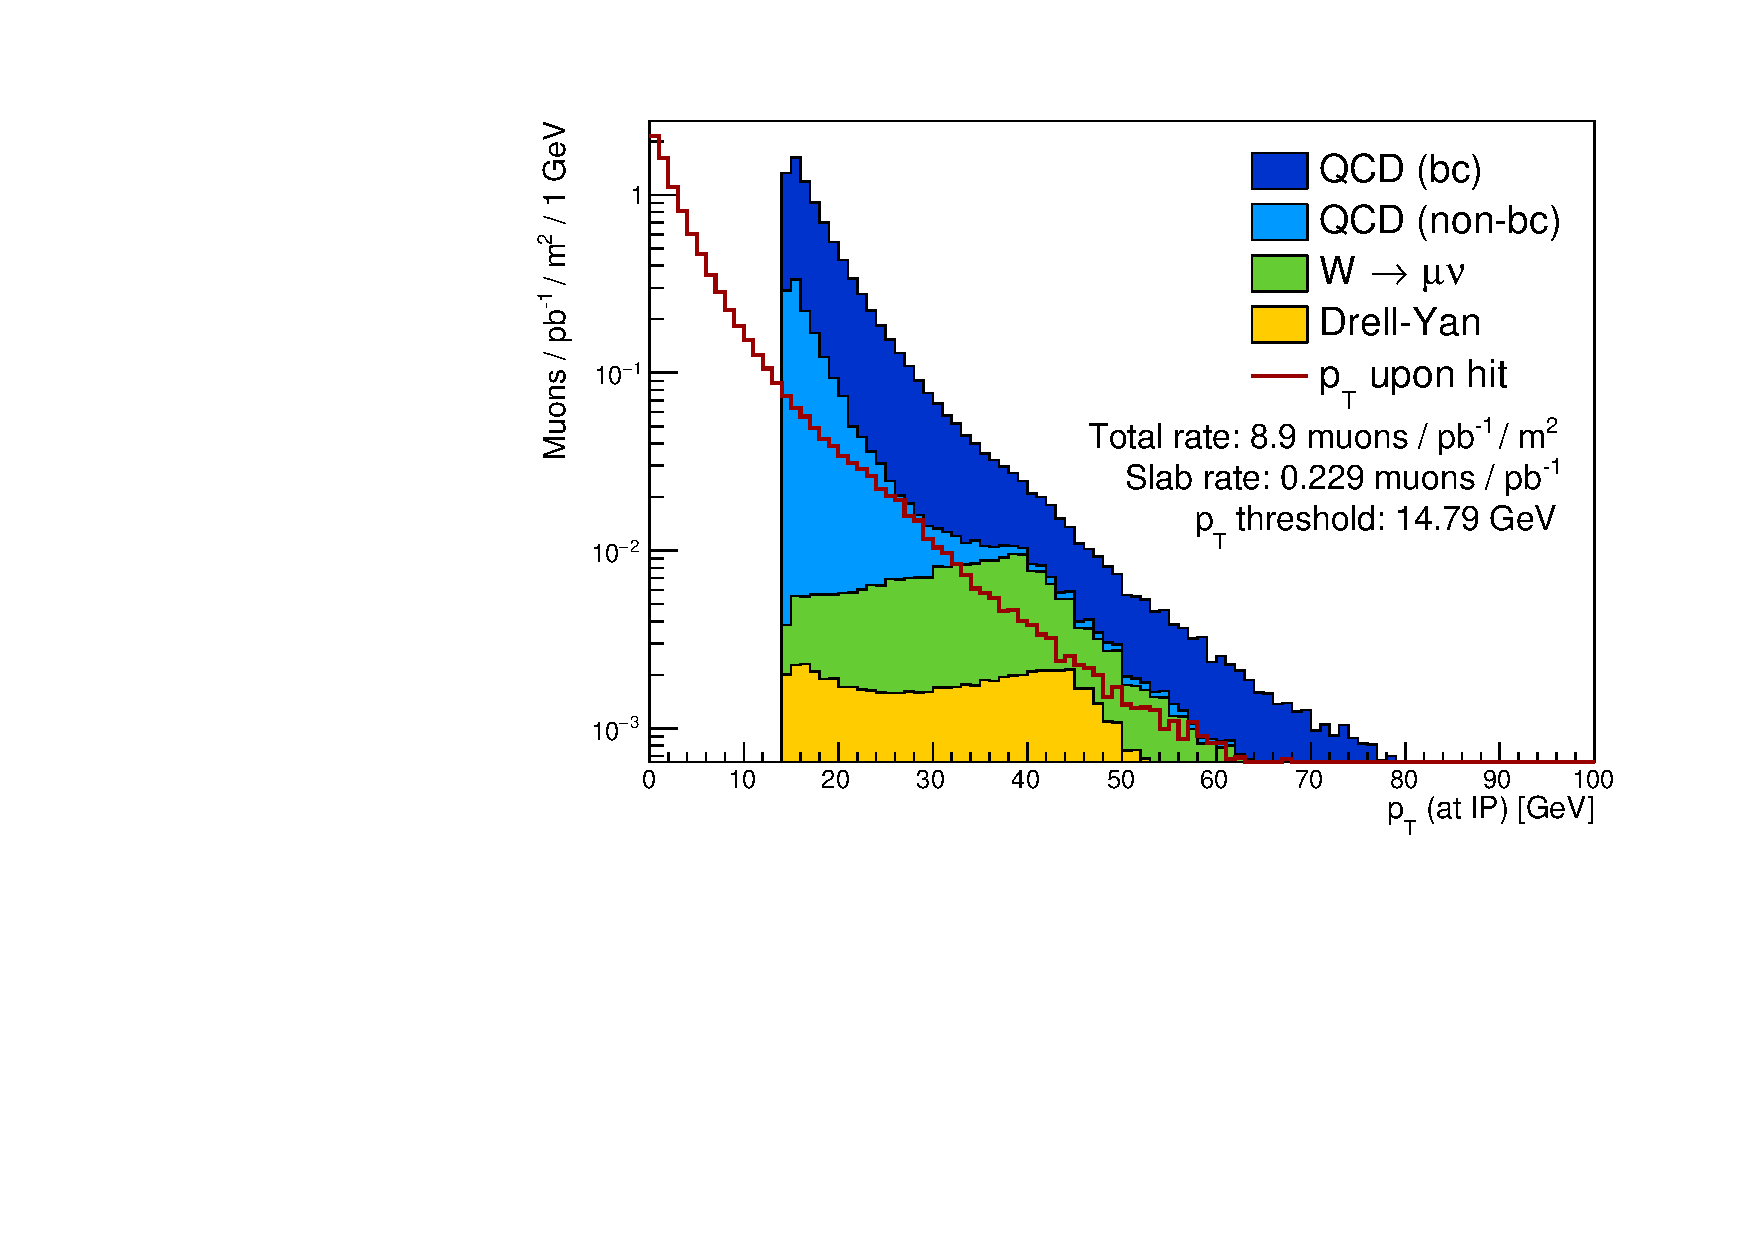
\includegraphics[width=0.60\textwidth]{figs/milliq/muon_pt.pdf}
    \caption{Rate of muons reaching the milliQan detector face as a function of production \pt,
      and broken down by production mode.
      There is a hard bound near 15\GeV due to energy loss in the material between
      the IP and milliQan. Above this threshold, the rate falls exponentially.
      The red curve shows the momentum upon intersection with milliQan, and is essentially
      the initial momentum distribution shifted left by $\sim$15\GeV.
            }
    \label{fig:mq_muon_ptdist}
  \end{center}
\end{figure}

Once mCP or muon four vectors are generated, they are propagated
through a model of the CMS and its environment, including
the magnetic field (see Fig.~\ref{fig:cms_bfield} for a colored map
of the magnetic field that is used), detector material, and 17 m of
rock between the IP and the drainage gallery.

The material geometry of CMS was extracted from a \textsc{Root} model,
and simplified into a series of concentric
iron cylinders, such that the total material budget is the same as that of the
real detector. Iron is placed at radii
\begin{itemize}\setlength\itemsep{-1mm}
\item $1.80 \leq r < 2.80$ m (tracker + HCAL)
\item $3.15 \leq r < 3.50$ m (magnet)
\item $3.85 \leq r < 4.05$ m (return yoke 1)
\item $4.60 \leq r < 4.95$ m (return yoke 2)
\item $5.35 \leq r < 5.95$ m (return yoke 3)
\item $6.35 \leq r < 7.15$ m (return yoke 4)
\end{itemize}

In addition to the iron, solid rock is placed at
$16 \leq r < 33$ m, until just before the face of the milliQan
detector.

Particles are propagated with a fourth-order Runge-Kutta
integrator, according to the relativistic kinematic equations
\be
\frac{d\vec{x}}{dt} = \vec{v} = \frac{\vec{p}c^2}{E} = \frac{\vec{p}c^2}{\sqrt{(\vec{p}c)^2+(mc^2)^2}}
\ee
\vspace{-6mm}
\be
\frac{d(\vec{p}c)}{dt} = 89.8755\;q\;\vec{v}\times\vec{B},
\ee
where the form of the second equation is valid if $B$ is in Tesla,
$t$ in ns, $\vec{v}$ in m/ns, $q$ in units of $e$, and $\vec{p}c$ in \MeV.

Multiple scattering is implemented using a small-angle Gaussian angle approximation,
as described in the PDG~\cite{PDGreview33}. At each time step, a $\theta_\mrm{RMS}$ is 
computed based on the particle momentum and charge, the radiation length of the material,
and the distance traversed. Then two random deflection angles are drawn from a Gaussian of width
$\theta_\mrm{RMS}$, one for each transverse direction. The particle is also displaced
a small amount in the transverse plane, in a way that is partially correlated with the
angular deflection.

Finally, at each timestep the particle loses energy according to the Bethe equation
\be
\left\langle-\frac{dE}{dx}\right\rangle = Kz^2\frac{Z}{A}\frac{1}{\beta^2}\left[\frac{1}{2}\log\frac{2m_ec^2\beta^2\gamma^2W_\text{max}}{I^2} - \beta^2 - \frac{\delta(\beta\gamma)}{2} \right],
\ee{equation}
where all terms and parameters are defined in the PDG~\cite{PDGreview33}.
Note that energy loss is a stochastic process, and at each timestep the actual energy loss follows a highly skewed Landau distribution.
However, the amount of material traversed in this application is quite large, so it should be sufficient to use the mean value
at each timestep. At any rate, a systematic is assessed on the interaction with matter that should cover for any inaccuracies
in the modeling of energy loss.

Particles (either muons or mCPs) are propagated until 2 m before the face of the milliQan detector
after which they are fed into a full \textsc{Geant4}~\cite{geant4} simulation of the detector.
This includes a full model of the drainage gallery, aluminum support structure,
scintillator bars/slabs/panels with wrapping, lead bricks, and PMTs.
Quantum efficiencies of the simulated PMTs are set individually on a per-channel
basis so that the average number of PEs generated by a cosmic and/or beam 
muon match that measured data, from the calibrations described in 
Sec.~\ref{sec:insitu_calib}. An illustration of a beam-based muon
traveling through the \textsc{Geant} model of the detector is 
shown in Fig.~\ref{fig:mq_geant}.

\begin{figure}[t]
  \begin{center}
    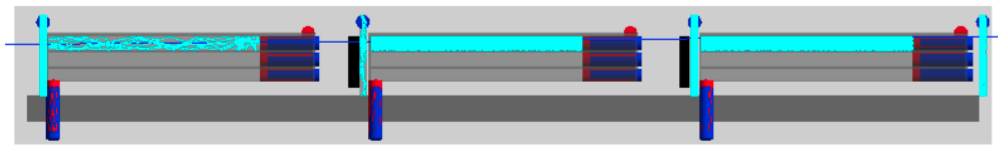
\includegraphics[width=0.750\textwidth]{figs/milliq/geant.png}
    \caption{Rendering of a beam-based muon traveling through
      a \textsc{Geant4} model of the demonstrator, hitting all
      four slabs and three bars in a straight line. Light blue
      lines are generated optical photons.
            }
    \label{fig:mq_geant}
  \end{center}
\end{figure}

The exact time of each detected photoelectron is saved, so that the \textsc{Geant} output
events can be used for \textit{pulse injection}, in which simulated PMT waveforms
are overlaid on zero-bias (i.e. random trigger) data, in order to generate realistic
detector signals that can be processed and analyzed with the same software as real data.
For each simulated PE, a random SPE area is drawn from PMT-specific
distributions derived via PMT bench tests, described in Sec.~\ref{sec:pmt_bench_tests}
(these distributions are corrected for slight differences between channels).
Then a template SPE waveform, also derived from the PMT bench tests, is scaled to this
area and overlaid on a random zero-bias event. These pulse-injected simulated events
then look just like real data, with the exception that they do not model
PMT saturation effects (however, this does not matter in practice).

\section{Simulation validation and data comparisons}

Simulation is validated by comparing various predicted quantities and distributions
to those measured in real data. The simplest comparison is the rate of muons coming
from the beam and passing through all four slabs of the detector. This probes the accuracy
of the muon cross sections and \pt distributions used for generation,
as well as the propagation routine and material model between the IP and milliQan.
The signal appears as four large pulses in the four slabs, with timing consistent
with a particle coming from the beam (roughly, $t_4-t_1=10\pm10$~ns); no requirement is
placed on hits in the bars or panels.

In data, the rate is measured at 0.18 muons/pb$^{-1}$, with negligible statistical
uncertainty. For the rate from simulation, we must account for various systematic
uncertainties. For the rate from heavy-flavor mesons, we scaled the cross section
by $1.25\pm0.25$ based on a comparison of FONLL with measured CMS data, so we take
a 20\% uncertainty. The rate from light-flavor mesons is sub-dominant but we take a
50\% uncertainty. Finally, we assess a systematic on the material modeling
of CMS and the rock by varying the density of all materials up and down by 7\%.
This translates to a 25\% uncertainty in muon rate due to the rapidly falling
momentum spectrum. All together, the predicted rate from simulation is
$0.25\pm0.08$ muons/pb$^{-1}$, agreeing with the rate measured in data
to within one standard deviation.

We can also roughly measure the angle of muons as they pass through milliQan,
which probes the accuracy of the multiple scattering and magnetic field modeling
of the propagation. We do this by looking at various ``patterns'' of bars
that record muon-like hits in each of the four-slab events. These patterns are shown
in diagrams on the $x$ axes of the plots in Fig.~\ref{fig:mq_muangles}. The left plot shows
milliQan from a top view, and the right plot from a side view. Black boxes mean we require
a muon hit in the given position, white boxes mean we require \textit{no} muon hit
in the given position, and a hashed boxes means it can be either. Muon hits are OR'd
over the orthogonal direction (so black actually means at least one hit over the relevant
bars, and white means no muon hits in any of the relevant bars).
We also make an adjustment to correct for imperfect modeling of muon ``fake rates''
(due to large muon-like hits from showering in a nearby bar) in simulation, which 
arises from the non-modeling of PMT saturation. The \Npe threshold in simulation
to count a hit as muon-like is adjusted until the ratio of the middle bin in the right
plot to the two neighboring bins is the same as in data (these all correspond to 
an angle of 0$^\circ$, but the middle bin has a lower rate due to the higher probability of a fake).
After making this correction, one sees that the observed angular distribution in data matches that
from simulation quite well. 

\begin{figure}[t]
  \begin{center}
    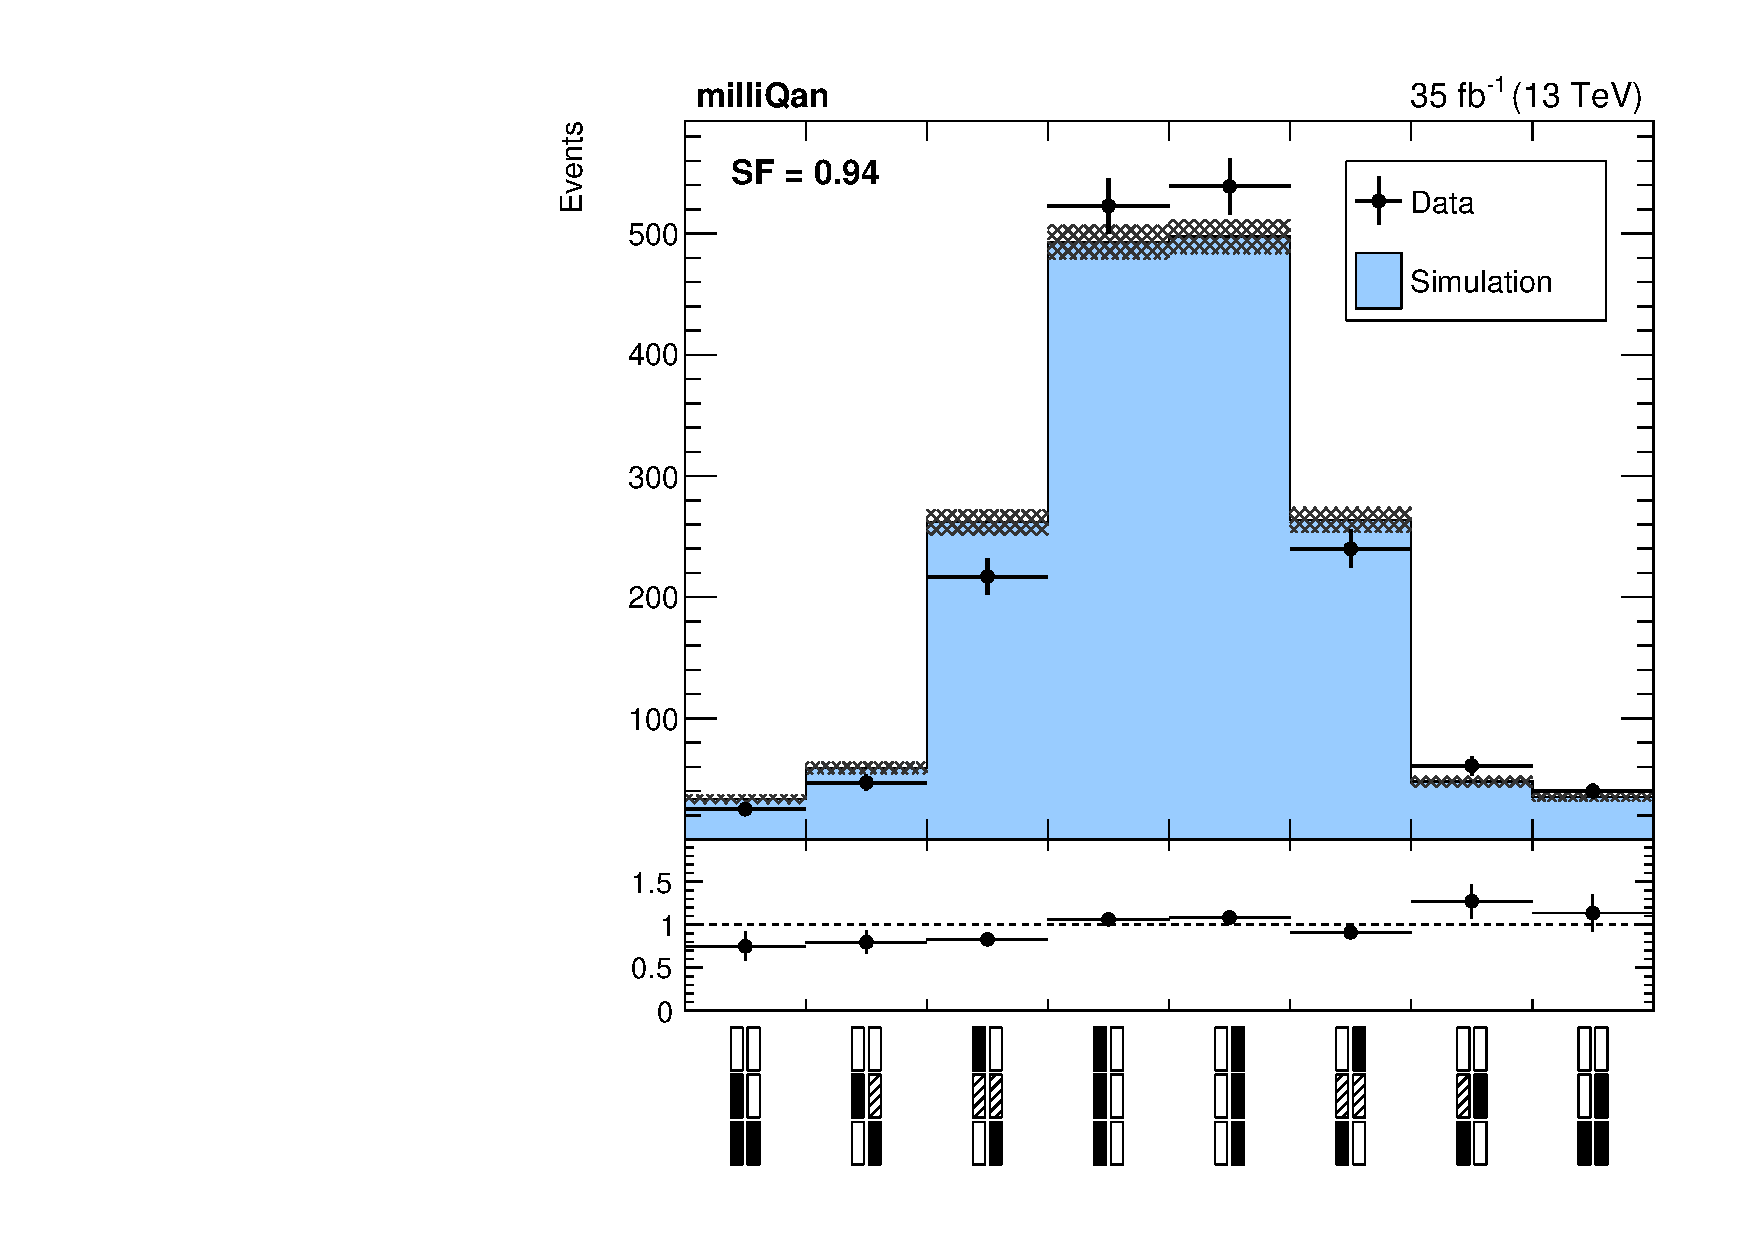
\includegraphics[width=0.495\textwidth]{figs/milliq/muangles_top.pdf}
    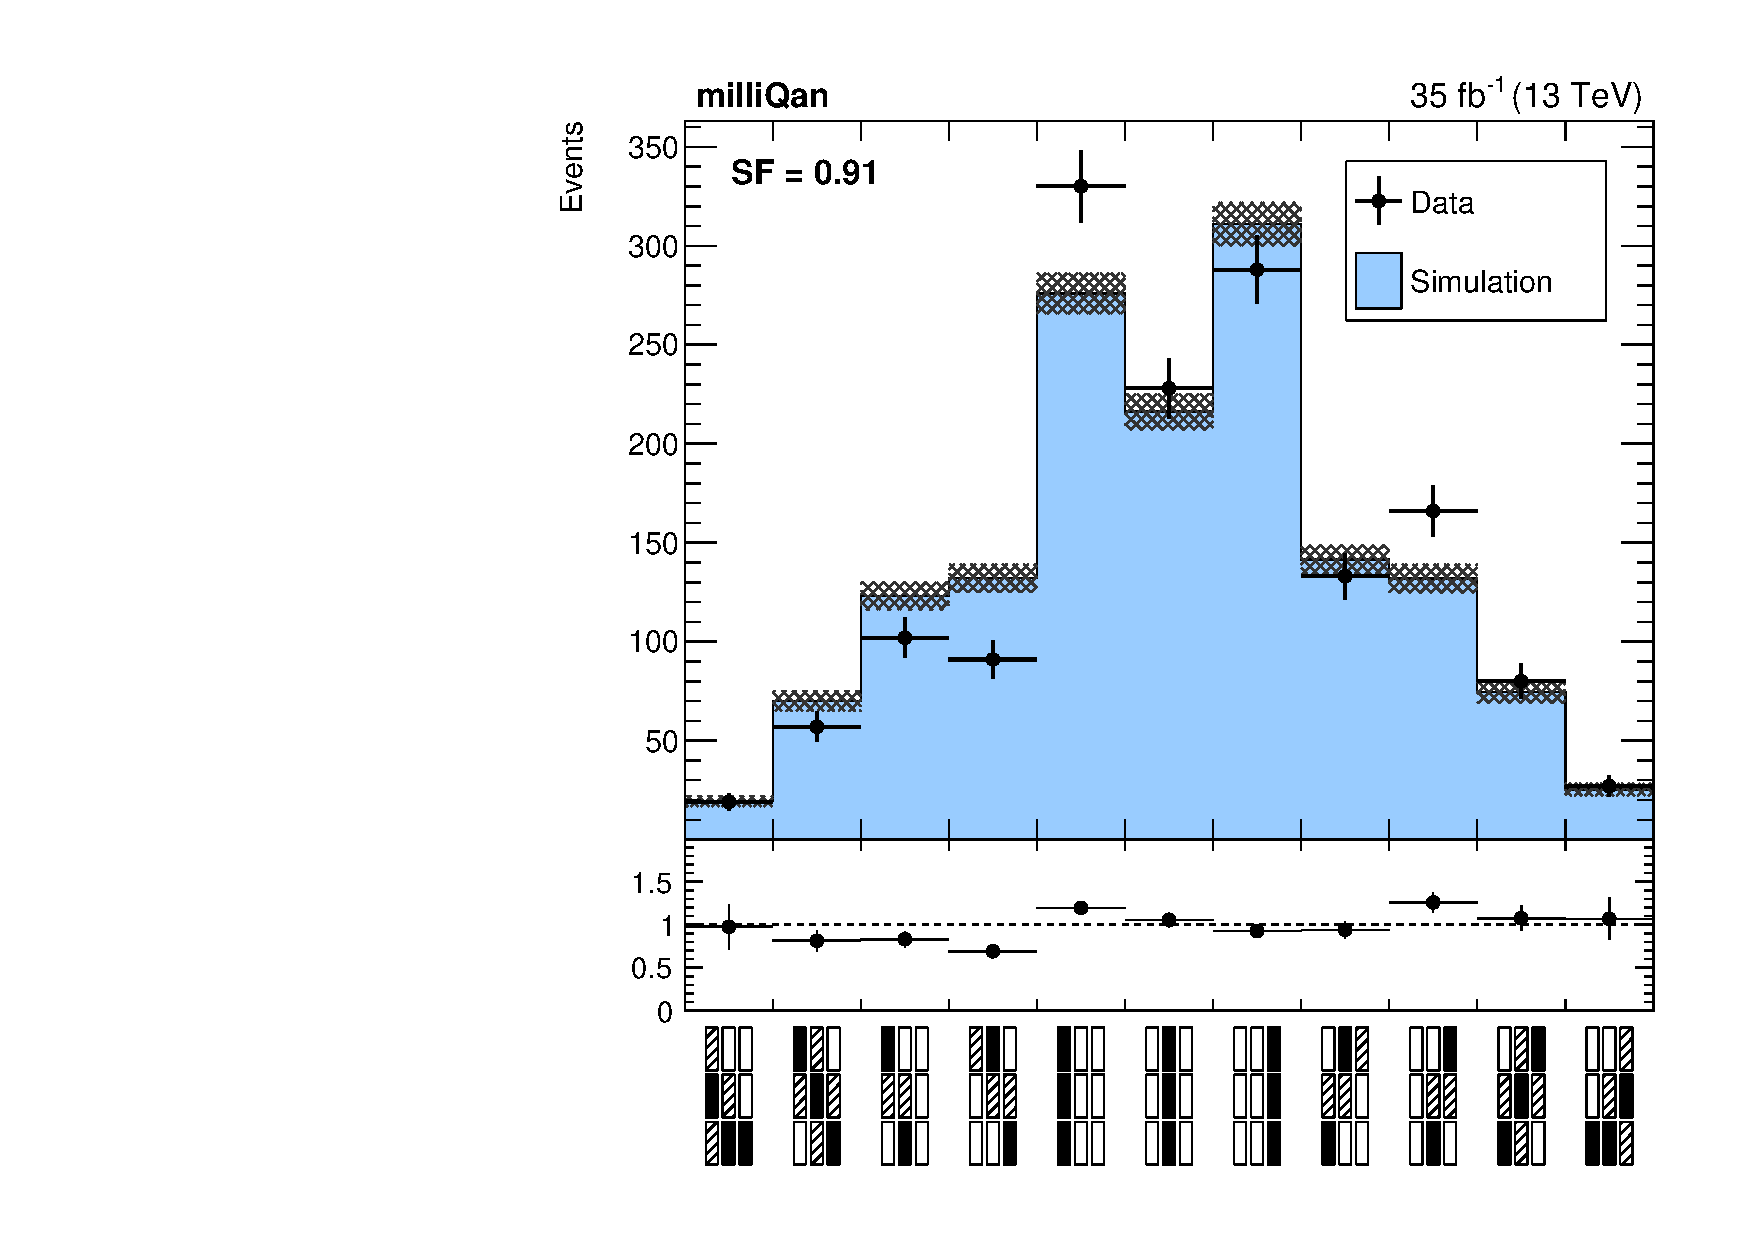
\includegraphics[width=0.495\textwidth]{figs/milliq/muangles_side.pdf}
    \caption{Rendering of a beam-based muon traveling through
      a \textsc{Geant4} model of the demonstrator, hitting all
      four slabs and three bars in a straight line. Light blue
      lines are generated optical photons.
            }
    \label{fig:mq_muangles}
  \end{center}
\end{figure}

We validate the \textsc{Geant4} simulation by looking at \Npe distributions
under various selections and comparing to data. Fig.~\ref{fig:npe_comps} shows
\Npe distributions in the bars for both data and simulation for four-slab beam muon
events, either in the case that the muon passes through all slabs and no bars, or
that the muon passes through a neighboring bar. The stacked histograms
are colored by computing the fraction of PEs in each event that come from various
production modes (generally, the muon knocks off an electron in some material, which
then either directly leaves energy deposits or bremsstrahlungs a gamma ray
that leaves deposits). Good agreement is seen everywhere, except at very low \Npe
($\lesssim30$). Hits in this regime are predominantly come from a muon knocking off
a very low-energy delta ray, which then bremsstrahlungs a low-energy gamma ray.
The modeling of this in \textsc{Geant4} is likely not reliable, leading
to the discrepancy. However, this is of minimal concern, as such kinds of processes
are irrelevant for the simulation of mCP events.

\begin{figure}[t]
  \begin{center}
    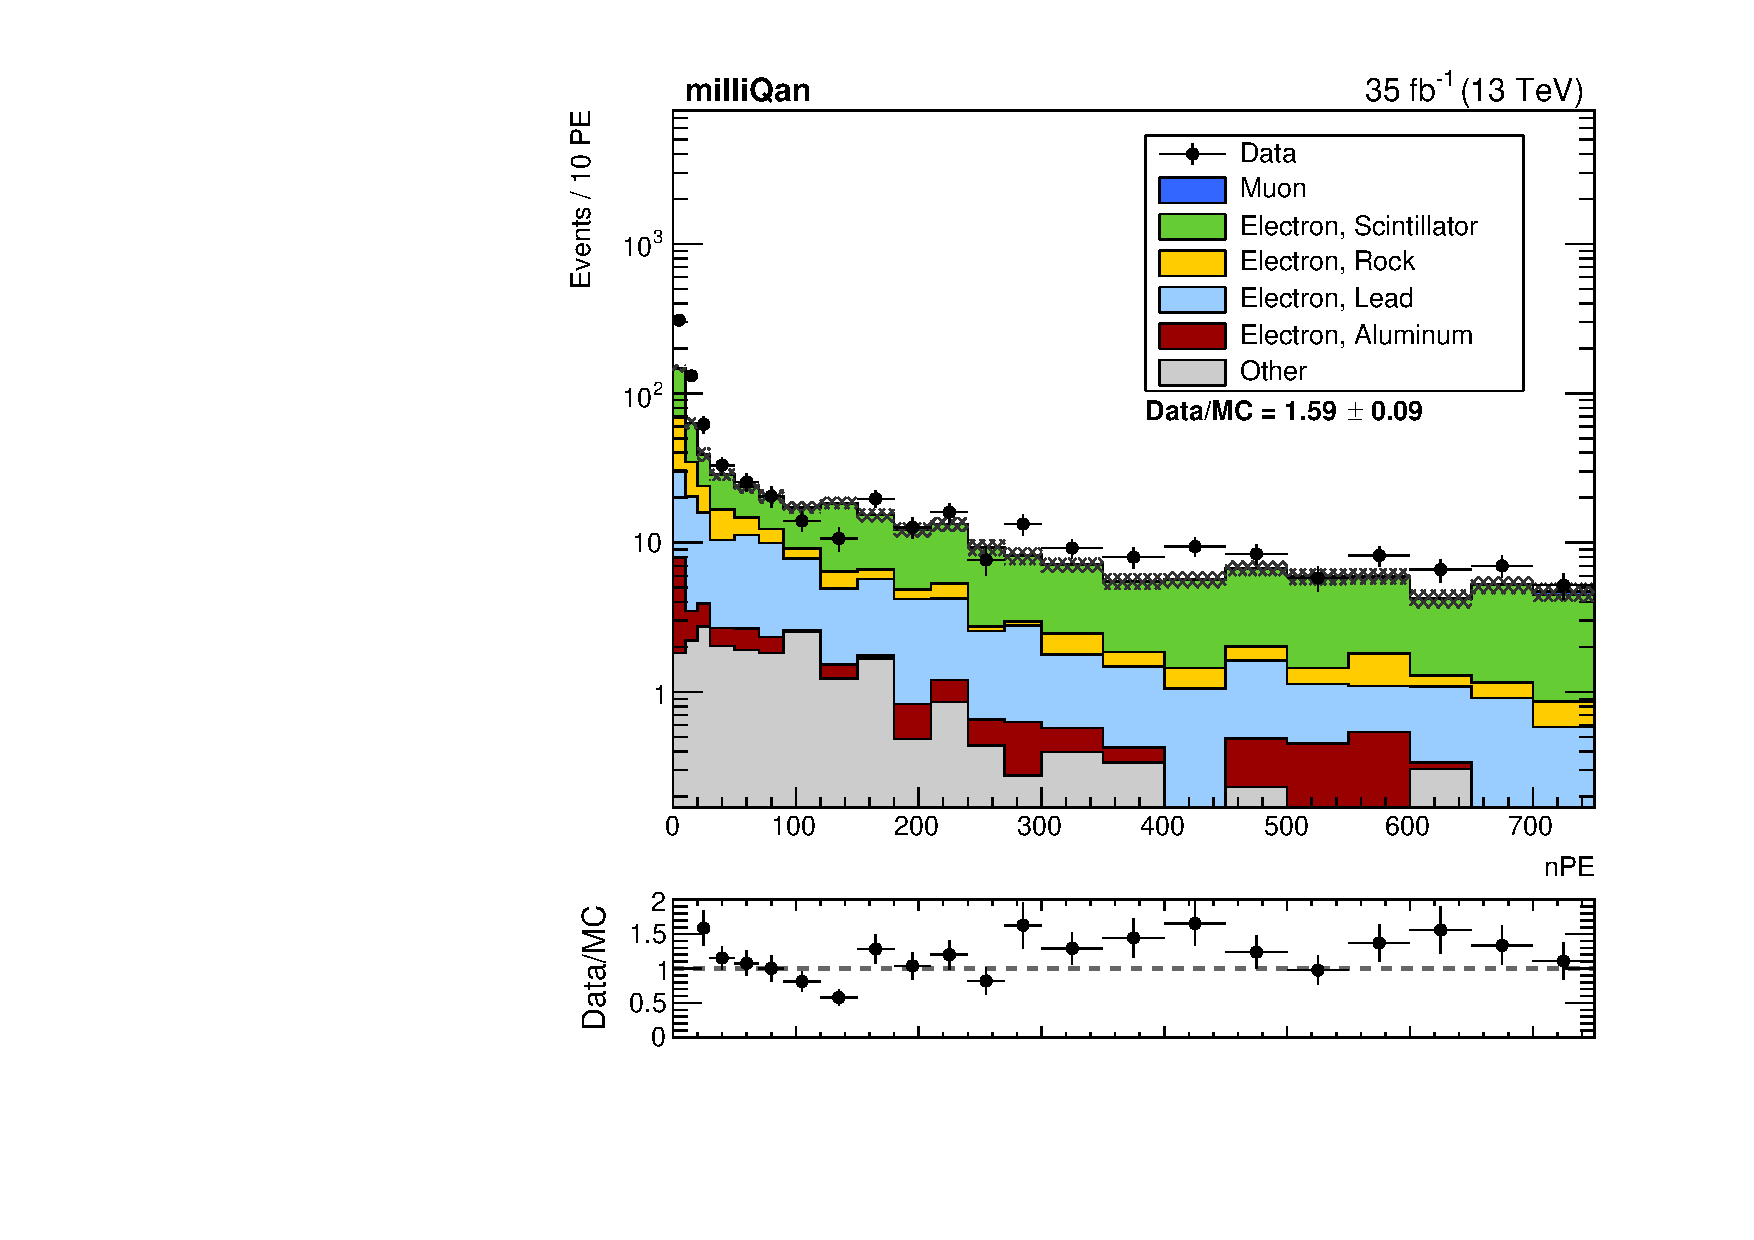
\includegraphics[width=0.495\textwidth]{figs/milliq/npe_comp_slabNoBar.pdf}
    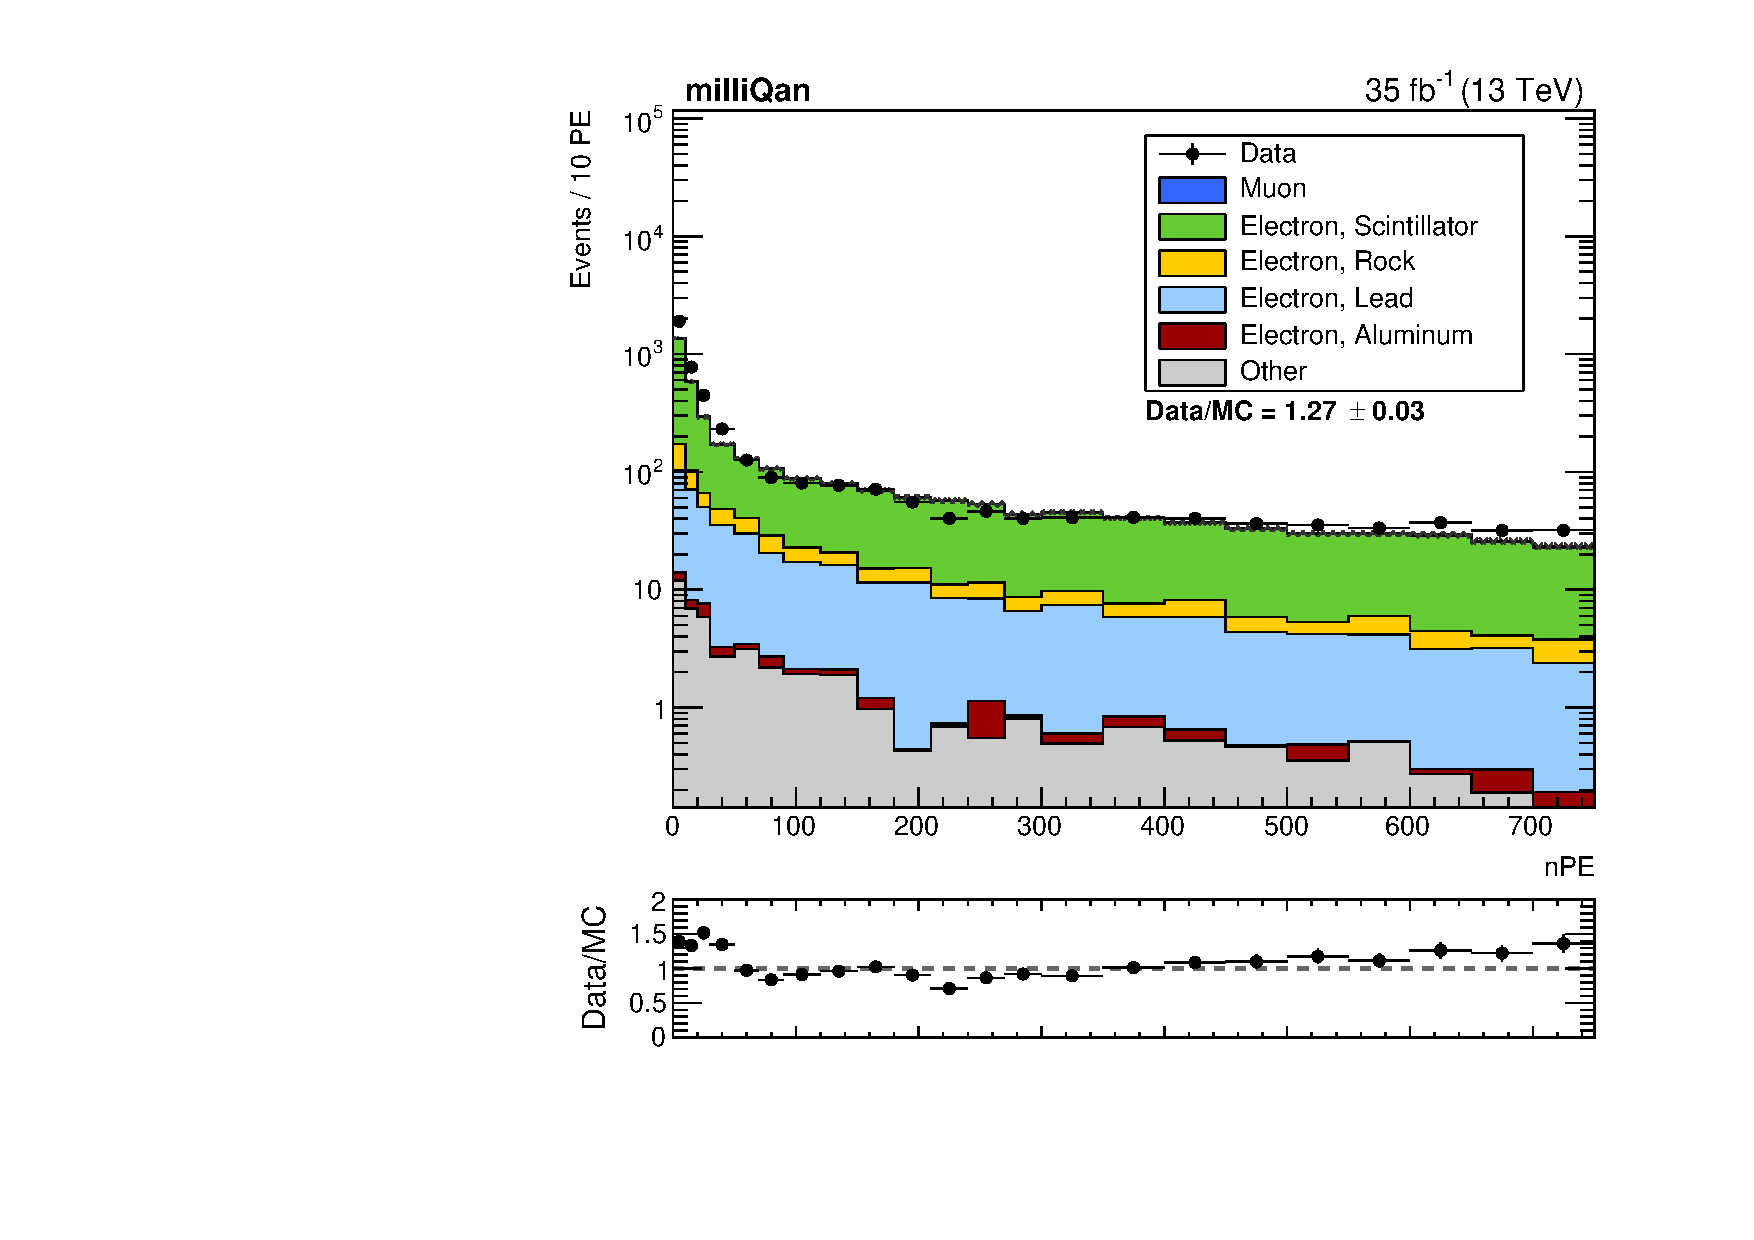
\includegraphics[width=0.495\textwidth]{figs/milliq/npe_comp_neighbBars.pdf}
    \caption{Comparison of \Npe distributions in the bars for events where
      (left) the muon hits all four slabs but no bars, and (right) the muon
      passes through a neighboring bar. Simulation is normalized by per-event weights
      computed from the cross sections of the various muon production modes described earlier.
      Good agreement is seen everywhere
      except at very low \Npe ($\lesssim30$). Such small hits are generally produced
      by low-energy delta rays knocked off by the muon, which bremsstrahlung
      low-energy gamma rays which then leave small deposits. \textsc{Geant4} modeling
      of these low-energy delta rays is not perfect, and in any case this is not
      relevant for the simulation of mCPs. The colors indicate the original source
      of each PE.
            }
    \label{fig:npe_comps}
  \end{center}
\end{figure}

\section{Background estimation and results}

A number of sources may be expected to produce a pulse in each layer of the demonstrator and therefore provide a background:
\begin{itemize}\setlength\itemsep{-1mm}
\item Dark rate overlap: each PMT has a dark current due to effects such as the thermal emission of electrons from the cathode. 
The simplest background source comes from random overlap of three such dark rate pulses. 
In addition, dark rate counts may overlap with a correlated double coincidence background from another source.
\item Cosmic/beam muon showers: a large number of gammas, neutrons and electrons may be caused by an interaction of a cosmic
ray muon with the rock in the demonstrator cavern. This may cause a pulse in each layer of the milliQan demonstrator. 
Such a background could also be expected from a beam muon which travels close to the demonstrator.
\item Radiation: radiation in the cavern, scintillator bars or surrounding material can cause correlated deposits in several bars. 
The lead blocks placed between layers should reduce the probability of a three layer deposit arising from photons or electrons, 
however, neutrons will not be shielded.
\item Afterpulses: afterpulses arising from correlated deposits may overlap and produce a triple coincidence signature 
in the demonstrator. The original correlated signature must not be triggered as in this case the afterpulses will fall 
in the readout deadtime and not be recorded.
\end{itemize}

\subsection{Signal region selections}

The backgrounds described above are largely reduced through the following baseline signal region selections:

\begin{itemize}\setlength\itemsep{-1mm}
\item Activity in exactly 1 bar per layer, and these bars must be in a straight line path
\item First pulse in each bar is the largest (i.e. no pre-pulses, but afterpulses are allowed)
\item No activity in any panel
\item No slab hit with $\Npe>250$
\item Max/min bar \Npe $<10$
\item max $\Delta t$(bars) $<15$ ns
\end{itemize}

The first requirement reduces combinatoric background, as almost all background is uncorrelated between layers.
The panel veto reduces contributions from cosmic and beam-based showers, and the slab veto removes
large pulses from throughgoing muons. The max/min bar \Npe and timing cuts again drastically reduce random
background, which is largely uncorrelated in both pulse size and time.

This baseline signal region is divided into 5 separate signal regions used for the final interpretation,
based on the number of slab hits and minimum bar \Npe. These are listed in Table~\ref{tab:mq_srdefs}.
The first two regions target small charges, roughly less than $\sim$0.01$e$, as these generally produce
no pulses in the slabs and small bar pulses. The second two regions target intermediate charges, 
roughly in the range 0.01 to 0.03$e$, which produce $\mathcal{O}(1)$ slab hit and slightly larger
bar pulses. The final region targets larger charges, which leave hits in two or more slabs.

\begin{table}[t]
\caption{The five orthogonal signal regions used in the analysis. They are
categorized based on number of slab hits (which must have $0.5<\Npe<250$) and the minimum \Npe over the three bars.
The final column lists the approximate mCP charge range probed by each signal region.
\label{tab:mq_srdefs}}
\centering
\begin{tabular}{c|cc|c}
%\hline
\hline
 SR & \# slab hits & min bar \Npe & Approx. targeted charge range\\
\hline
1 & 0 & $[2,\;20]$ & $\leq0.014$\\
2 & 0 & $>20$ & 0.014--0.03\\
3 & 1 & $[5,\;30]$ & 0.01--0.02\\
4 & 1 & $>30$ & 0.02--0.05\\
5 & $\geq$2 & $>0.5$ & $\geq0.03$\\
\hline
\end{tabular}
\end{table}

\subsection{Background estimation method}
\label{sec:mq_bkg_est}

The expected background counts in each region are estimated by an ``ABCD'' method, in which the
observed counts in orthogonal non-pointing regions are scaled by transfer factors measured
in inverted-$\Delta t$ regions. Specifically, we define regions
\begin{itemize}\setlength\itemsep{-1mm}
\item A: pointing, max $\Delta t$(bars) $<15$ ns
\item B: non-pointing, max $\Delta t$(bars) $<15$ ns
\item C: pointing, max $\Delta t$(bars) $>15$ ns
\item D: non-pointing, max $\Delta t$(bars) $>15$ ns
\end{itemize}
where ``pointing'' refers to the requirement that the single bars in each layer form a straight line path,
and max $\Delta t$(bars) is the maximum time difference between any two bars. Additional requirements
on the number of slabs and minimum bar \Npe are added to each region for estimating the individual signal
regions listed in Table~\ref{tab:mq_srdefs}.

Region A is the region whose background count we want to estimate, and B, C, and D are orthogonal control regions. 
Assuming that the timing distribution is not correlated with whether or not the pointing requirement is satisfied, 
we can estimate
\be
N_\mrm{A} = \frac{N_\mrm{C}}{N_\mrm{D}} N_\mrm{B}.
\ee

We check that the method works in a beam-off control region; results are shown in
Table~\ref{tab:mq_abcd_valid}. Good agreement between predicted and observed counts
is seen in all regions. We must also verify that there are no significant beam-based
backgrounds that would break the method. To do this, we compare predictions between
beam-off and beam-on data, adjusted for total data collection time. Again we see
good agreement, indicating that any beam-based backgrounds are negligible.
In any case, we verify from simulation that adding beam-based backgrounds
to the non-beam backgrounds preserves the validity of the ABCD method.

\begin{table}[t]
\caption{Two validations of the ABCD background estimation method:
comparisons of predicted vs. observed in a beam-off control region
(shows that the method works with non-beam backgrounds), and comparisons
of predictions from beam-off and beam-on data (shows that beam-based
backgrounds are negligible). Uncertainties shown are statistical.
\label{tab:mq_abcd_valid}}
\centering
\renewcommand{\arraystretch}{1.3}
\begin{tabular}{c|cc|c}
\multirow{2}{*}{SR} & \multicolumn{2}{c}{Beam off} & Beam on \\
%% \hline
\cline{2-4}
 & Pred. & Obs. & Pred. \\
\hline
1 & $121.2^{+6.0}_{-5.9}$ & 131 & $124.2^{+5.6}_{-4.0}$ \\
2 & $47.4^{+5.2}_{-4.8}$ & 45 & $49.9^{+5.5}_{-4.8}$ \\
3 & $7.8^{+2.5}_{-1.8}$ & 9 & $10.7^{+3.2}_{-2.0}$ \\
4 & $2.7^{+2.1}_{-1.1}$ & 4 & $2.4^{+1.8}_{-0.8}$ \\
5 & $0.8^{+1.4}_{-0.4}$ & 1 & $0.0^{+0.9}_{-0.0}$ \\
\hline
\end{tabular}
\end{table}

We additionally perform the validations as a function of minimum bar \Npe. Comparisons of
minimum bar \Npe distributions, between predictions/observations in beam-off data
as well as predictions between beam-off and beam-on data, are shown in 
Fig~\ref{fig:mq_abcd_valid}. This is done for the 0- and 1-slab regions,
but not the $\geq$2 slab region as there are not enough events.

\begin{figure}[t]
  \begin{center}
    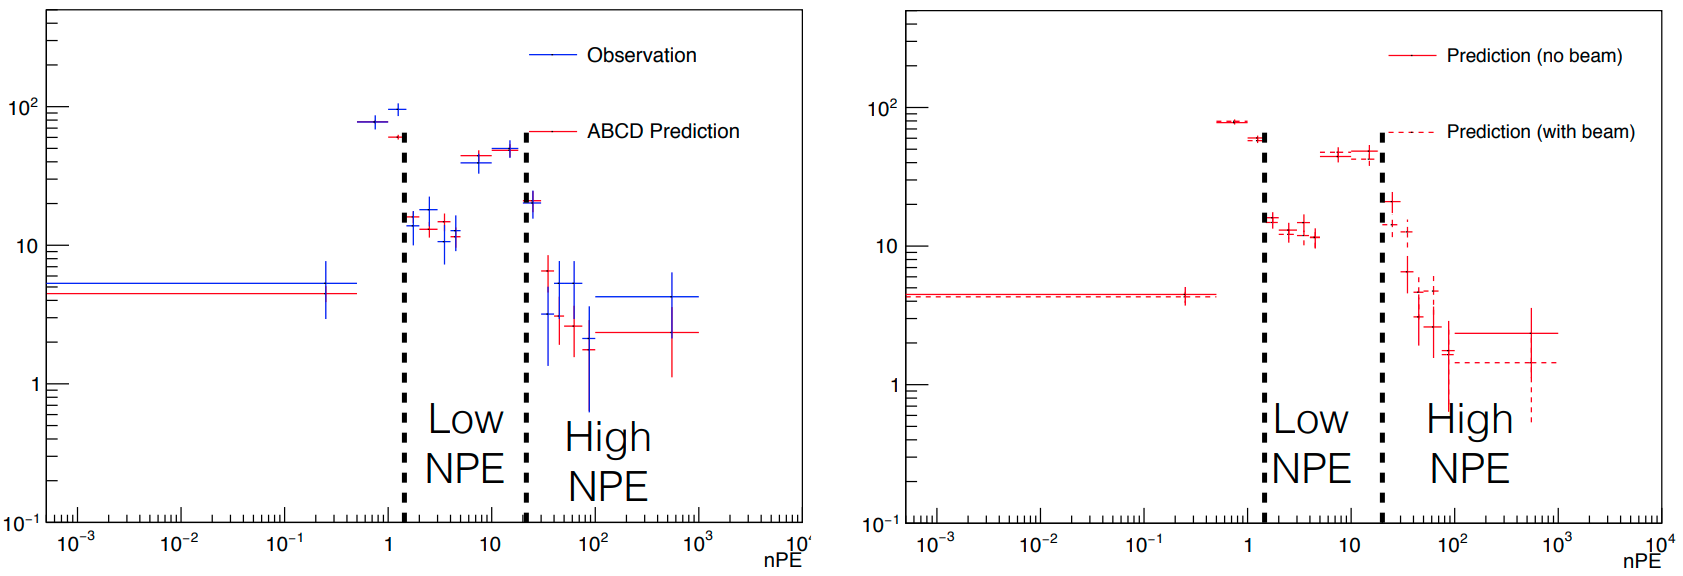
\includegraphics[width=0.95\textwidth]{figs/milliq/abcd_valid_0slab.png} \vskip2mm
    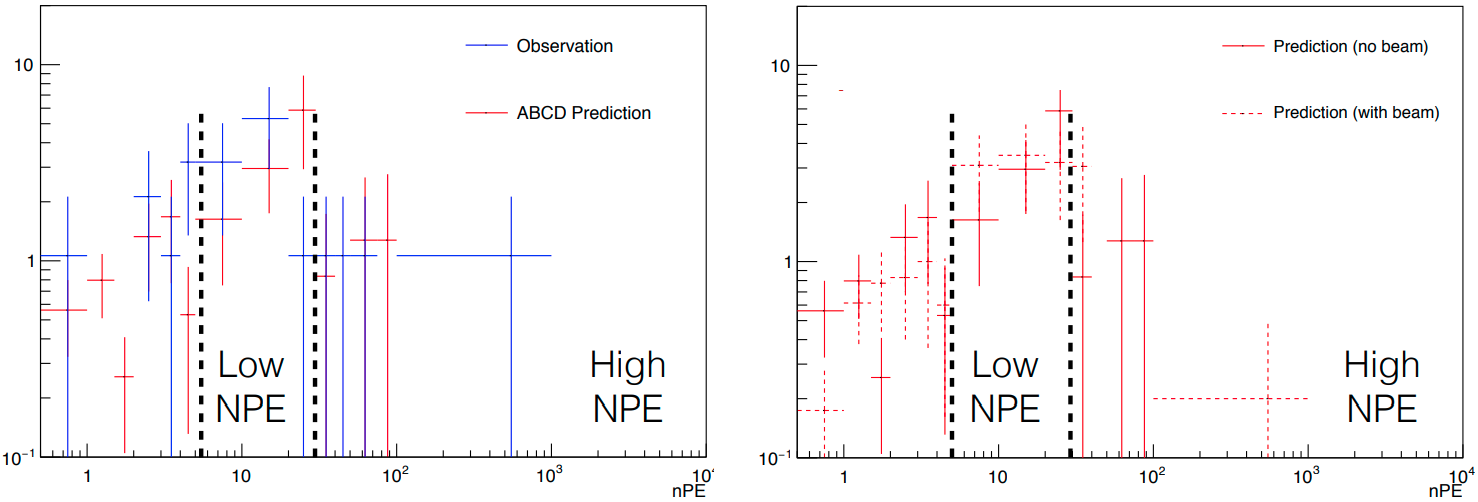
\includegraphics[width=0.95\textwidth]{figs/milliq/abcd_valid_1slab.png}
    \caption{ABCD method validations as a function of minimum bar \Npe.
      The left plots show beam-off predictions/observations, and the right
      plots compare predictions from beam-on and beam-off data.
      On the top are the 0 slab regions, and the bottom the 1 slab regions.
      The $\geq$2 slab region does not have enough statistics to allow
      a full \Npe distribution. Vertical dashed lines indicate
      the boundaries of the signal regions (regions 1 and 2 for the top plots,
      and 3 and 4 for the bottom plots). Integrated predictions and
      observations for these regions are listed in Table~\ref{tab:mq_abcd_valid}.
            }
    \label{fig:mq_abcd_valid}
  \end{center}
\end{figure}


\subsection{Systematic uncertainties}
\label{sec:mq_systs}

We assess a number of systematic uncertainties both on the background estimate and the
signal yield prediction. On the background estimate, the primary uncertainty arises
from the statistical uncertainty on the ABCD prediction, especially for the $\geq$1
slab regions where statistics are lower. These uncertainties are given
in the final column of Table~\ref{tab:mq_abcd_valid}. Additionally, we assess a systematic
based on the small prediction/observation disagreements in the beam-off data.

For the signal yield prediction, we assess a systematic uncertainty on the differential cross
section of each production mode individually, as well as an overall proton-proton inelastic
cross section uncertainty used for the light meson production modes. Details are given in
Sec.~\ref{sec:mq_mcgen}. 

A material modeling systematic is assigned by varying the density
of material between the CMS IP and milliQan up and down by 7\%, re-running the signal simulation
and observing the change in signal region yields (7\% is chosen based on uncertainty in both the
distance and density of the intervening rock). This is negligible for all but the highest charges considered
($>$0.1$e$), and even for these it remains a sub-leading source of uncertainty.

We also account for uncertainties in the per-channel \Npe calibrations, but this is non-trivial
to propagate to final signal region yields. The uncertainty on each channel's calibration
comes from a number of sources, some correlated and some not:
\begin{itemize}\setlength\itemsep{-1mm}
\item Statistical uncertainty from fit: 10--20\%, uncorrelated everywhere
\item Correction of SPE mean: 1--5\%; arises from the fact that the mode of the 
SPE area distribution (measured in-situ) differs from the mean (measured in the lab)
by up to 10\%, due to a large left tail in the area distributions. We correct for this, and take half the difference
as an uncertainty. This is correlated between bars with the same PMT species.
\item B/no-B differences: typically $<$10\%, but up to 20\%. Arises from differences in measured
SPE values between magnetic field on/off runs. Uncorrelated everywhere.
\item Low-pass filter: 5--20\%, only on R878s (and fully correlated between them). A low-pass filter
is applied to the waveforms for calibration, but not in the main analysis. We take the difference
in measured SPE values with/without the filter as a systematic. R7725s and ETs are unaffected
as their SPE pulses are much larger and cleaner.
\item Global fully-correlated 5\% uncertainty, from observed differences in the power law
fits between cosmic and SPE points.
\end{itemize}

To translate these per-channel uncertainties into signal region yield uncertainties, we generate
1000 ``calibration toys'' in which the PMT efficiencies are varied according to the model above,
taking into account all correlations. Signal region yields are recorded for each toy, and the
covariance matrix of the yields is diagonalized to generate $N_\mrm{SR}$ independent uncertainties,
fully accounting for correlations between the various signal region yields.
Scatterplots of signal region yields from such toys for an example (mass, charge) point
are shown in Fig.~\ref{fig:mq_calib_toys}.

\begin{figure}[t]
  \begin{center}
    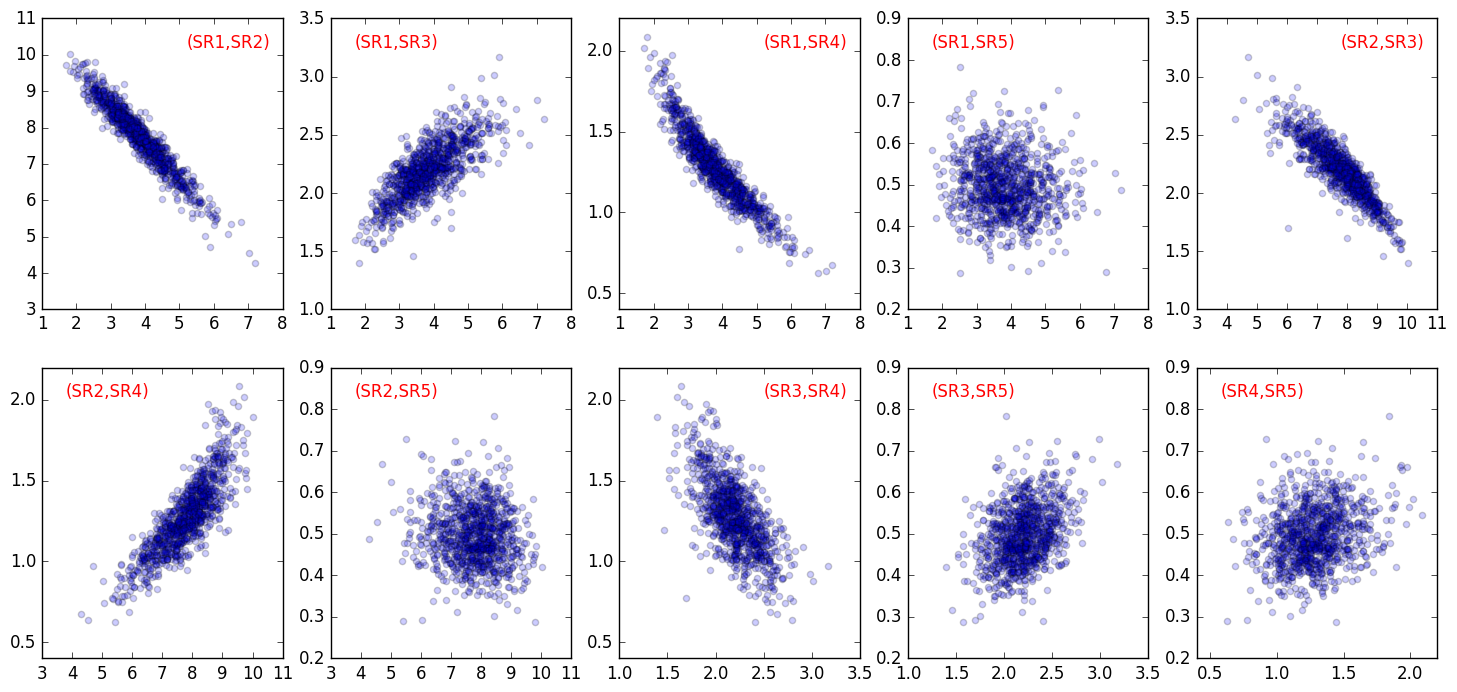
\includegraphics[width=0.95\textwidth]{figs/milliq/calib_toys.png}
    \caption{Scatterplots of signal region yields in 1000 \Npe calibration toys,
      for an example signal point $m=1.0\GeV$, $q=0.014e$. Diagonalizing the covariance
      matrix gives five independent uncertainties, accounting for all correlations
      between the various regions (e.g. the dominant uncertainty in this example shifts events
      from regions 1 and 3 to 2 and 4, i.e. between the low bar \Npe and high bar \Npe
      regions, arising from correlated calibration uncertainties between the bars).
            }
    \label{fig:mq_calib_toys}
  \end{center}
\end{figure}

Finally, we assess a systematic uncertainty on the time smearing correction applied to signal simulation.
As the time resolution discrepancies between simulation and data have an unknown origin,
the full size of the correction is used as a systematic uncertainty.

\subsection{Results and limits}

Predictions are made from the beam-on dataset, representing 37 fb$^{-1}$ of proton-proton collision data
taken in 2018, using the ABCD method described in
Sec.~\ref{sec:mq_bkg_est}. In addition to the statistical uncertainty from
the limited size of the control regions, an additional systematic uncertainty is
assigned based on small disagreements between prediction and observation
in the beam-off validation (Table~\ref{tab:mq_abcd_valid}). Predictions and their total
uncertainties are listed in Table~\ref{tab:mq_results}, along with the observed event counts.
The observed counts agree with predictions within the uncertainty in all cases.

\begin{table}[t]
\caption{Predictions and observations in the 5 orthogonal signal regions.
Uncertainties shown in the predictions include both statistical uncertainty
from the limited size of the control regions, and systematic uncertainty from small disagreements
in the beam-off validation.
The observed event counts are consistent with the predicted counts in all cases.
The final three columns give estimated signal yields for three $(m_\mrm{mCP},Q)$ points
near the exclusion boundary.
\label{tab:mq_results}}
\centering
\renewcommand{\arraystretch}{1.3}
\resizebox{\textwidth}{!}{%
\begin{tabular}{c|cc|cc|ccc}
%\hline
\multicolumn{5}{c}{} & \multicolumn{3}{c}{Signal yields ($m_\mrm{mCP}$ [GeV], $Q/e$)} \\
\hline
 SR & \# slab hits & min bar \Npe & Pred. & Obs. & (0.05, 0.007) & (1.0, 0.02) & (3.0, 0.1)\\
\hline
1 & 0 & $[2,\;20]$ & $124\pm11$ & 129 & 60.0 & 0.4 & 0 \\
2 & 0 & $>20$ & $49.9^{+6.0}_{-5.4}$ & 52 & 0 & 16.3 & 0 \\
3 & 1 & $[5,\;30]$ & $10.7^{+3.6}_{-2.6}$ & 8 & 0.5 & 0.5 & 0 \\
4 & 1 & $>30$ & $2.4^{+2.1}_{-1.1}$ & 4 & 0 & 8.5 & 0 \\
5 & $\geq$2 & $>0.5$ & $0.0^{+0.9}_{-0.0}$ & 1 & 0.6 & 1.9 & 4.2 \\
\hline
\end{tabular}}
\end{table}


}

The results are interpreted using the signal production model discussed in Sec.~\ref{sec:mq_mcgen}, with the systematic uncertainties on signal yields listed in
Sec.~\ref{sec:mq_systs}.
Under the signal plus background hypothesis, a modified frequentist approach is used
to determine observed upper limits at 95\% confidence level
on the cross section to produce a pair of mCPs, as a function of mass and charge. 
The approach uses the the CLs
technique, described in Sec. \ref{sec:fits}. The observed upper limits are evaluated
through the use of asymptotic formulae. Figure~\ref{fig:mq_limit} shows the exclusion at 95\% 
confidence level in mass and charge of the mCP. 
The existence of new particles with mass between 20 and 3000~MeV is excluded for minimum charge varying
 between $0.006e$ and $0.3e$, depending on mass.
Compared to existing constraints, 
the milliQan demonstrator provides unique sensitivity for mCP masses above 0.7 GeV.

\begin{figure}[t]
  \begin{center}
    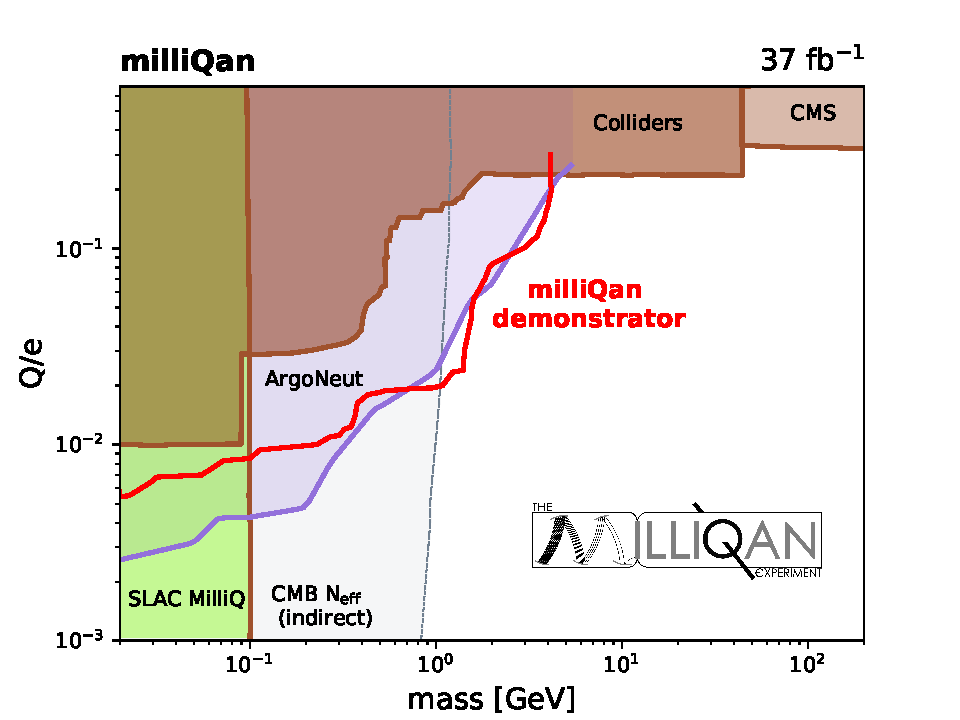
\includegraphics[width=0.70\textwidth]{figs/milliq/finalLimit.pdf}
    \caption{Exclusion in the mCP $(m,Q)$ plane at the 95\% confidence level compared
      to existing constraints from colliders, CMS~\cite{Chatrchyan_2013,Chatrchyan_2013_2}, ArgoNeuT~\cite{ArgoNeuT}, and SLAC MilliQ~\cite{MilliQ},
      as well as the indirect constraint from the CMB relativistic degrees of freedom~\cite{Brust:2013ova}.
            }
    \label{fig:mq_limit}
  \end{center}
\end{figure}
